\section{The ATLAS detector and data taking}
\label{chapter:detector}

The Large Hadron Collider (LHC)~\cite{Evans:2008zzb} at CERN is currently the world's newest, largest and most powerful collider, located near Geneva, Switzerland. It is designed to collide proton-proton with a center of mass of 14 TeV and an unprecedented luminosity of $10^{-34}\text{cm}^{-2}\text{s}^{-1}$. It can also collide heavy ions, like Pb+Pb and Xe+Xe, with an energy of several TeV per nucleon and a peak luminosity of $10^{-27}\text{cm}^{-2}\text{s}^{-1}$. In this section, we aim to describe the designs of LHC and ATLAS detector, as well as the data acquisition and selection procedure.

\subsection{The Large Hadron Collider}

The LHC~\cite{Evans:2008zzb} is a two-ring-superconducting-hadron accelerator and collider installed in the existing 26.7 km tunnel that was constructed between 1984 and 1989 for the CERN LEP machine. The LEP tunnel has eight straight sections and eight arcs and lies between 45 m and 170 m below the surface on a plane inclined at $1.4\%$ sloping. LHC contains two counter-propagating beams containing bunches of protons or ions that cross each other at four points, where collisions take place. At these crossing points, located four LHC detectors: ATLAS, CMS, ALICE and LHCb. ALICE is specially designed for the heavy-ion program, while ATLAS and CMS are mainly targeted for proton collisions, and will collect heavy-ion data for about one month each year. The bending power for the beams is provided by 1232 superconducting dipole magnets, each 15 m long and capable of generating 8.3 T magnetic fields. To focus the beam, quadrupole magnets are implemented. Accelerating cavities are used to compensate for the energy loss and keep the bunches at a constant energy.

In Run 2, Pb ion can achieve the energy up to 5.02 TeV per nucleon. Ions are boosted in a sequence of accelerators before injected into the LHC. An example of the sequence is shown in Figure~\ref{fig:detector_cartoon_LHC}, where Pb ions go through LINAC3, LEIR, PS, SPS and LHC, with the energy being ramped up at each stage: 4.2 MeV, 72 MeV, 6 GeV, 177 GeV and 2.76 TeV.

\begin{figure}[H]
\centering
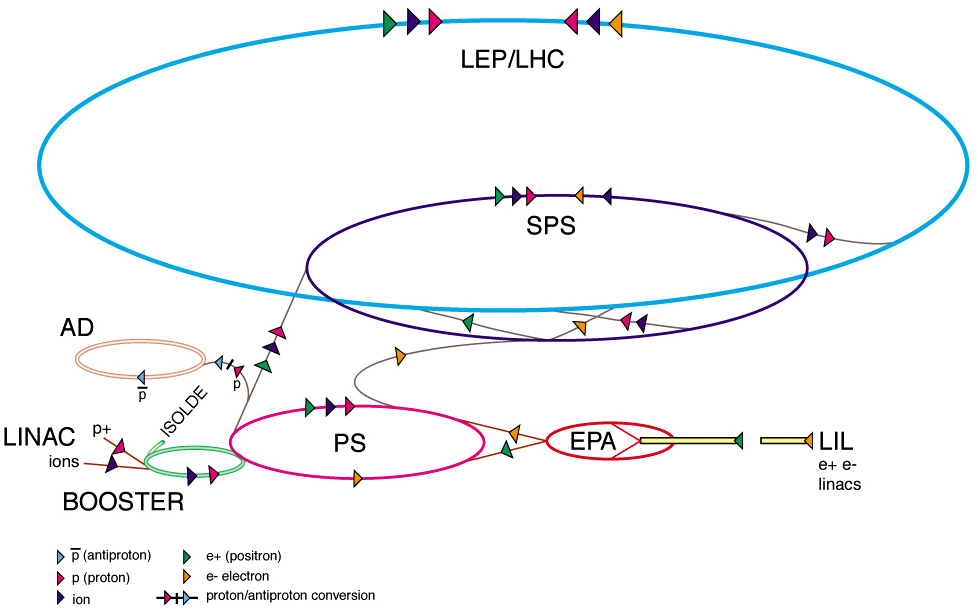
\includegraphics[width=.95\linewidth]{figs/chapter_detector/cartoon_LHC.jpg}
\caption{The CERN accelerator sequence. The figure is taken from Ref.~\cite{Jean-Luc:841493}.}
\label{fig:detector_cartoon_LHC}
\end{figure}



\subsection{The ATLAS detector}

The physics goals of heavy-ion program can be turned into a set of general requirements for the LHC detectors:
\begin{itemize}
\item Due to the experimental conditions, the detectors require fast, radiation-hard electronics and sensor elements.
\item High detector granularity is needed to handle the particle fluxes and to reduce the influence of overlapping events;
\item Large acceptance in pseudorapidity with almost full azimuthal angle coverage is required;
\item Good charged particle momentum resolution and reconstruction efficiency in the inner tracker are essential;
\item Highly efficient triggering on low transverse-momentum objects with sufficient background rejection;
\end{itemize}

ATLAS (A Toroidal LHC ApparatuS)~\cite{Aad:2008zzm} is a multi purpose detector located at Point-1 of the LHC cavern. While mainly designed to study the $pp$ collisions, its fine granularity and large acceptance makes it an ideal detector for study Pb+Pb and $p$Pb collisions as well. The overall ATLAS detector layout is shown in Figure~\ref{fig:detector_ATLAS_detector}. The ATLAS detector is nominally forward-backward symmetric with respect to the interaction point, and covers the full azimuthal angle. The magnet configuration comprises a thin superconducting solenoid surrounding the inner-detector cavity, and three large superconducting toroids (one barrel and two end-caps) arranged with an eight-fold azimuthal symmetry around the calorimeters. This fundamental choice has driven the design the rest of the detector. In this section, only the subsystems that are used in this work are described:
\begin{itemize}
\item Inner Detector (ID);
\item Forward Calorimeter (FCal);
\item Zero-Degree Calorimeter (ZDC);
\item Minimum-Bias Trigger Scintillators (MBST);
\end{itemize}

\begin{figure}[H]
\centering
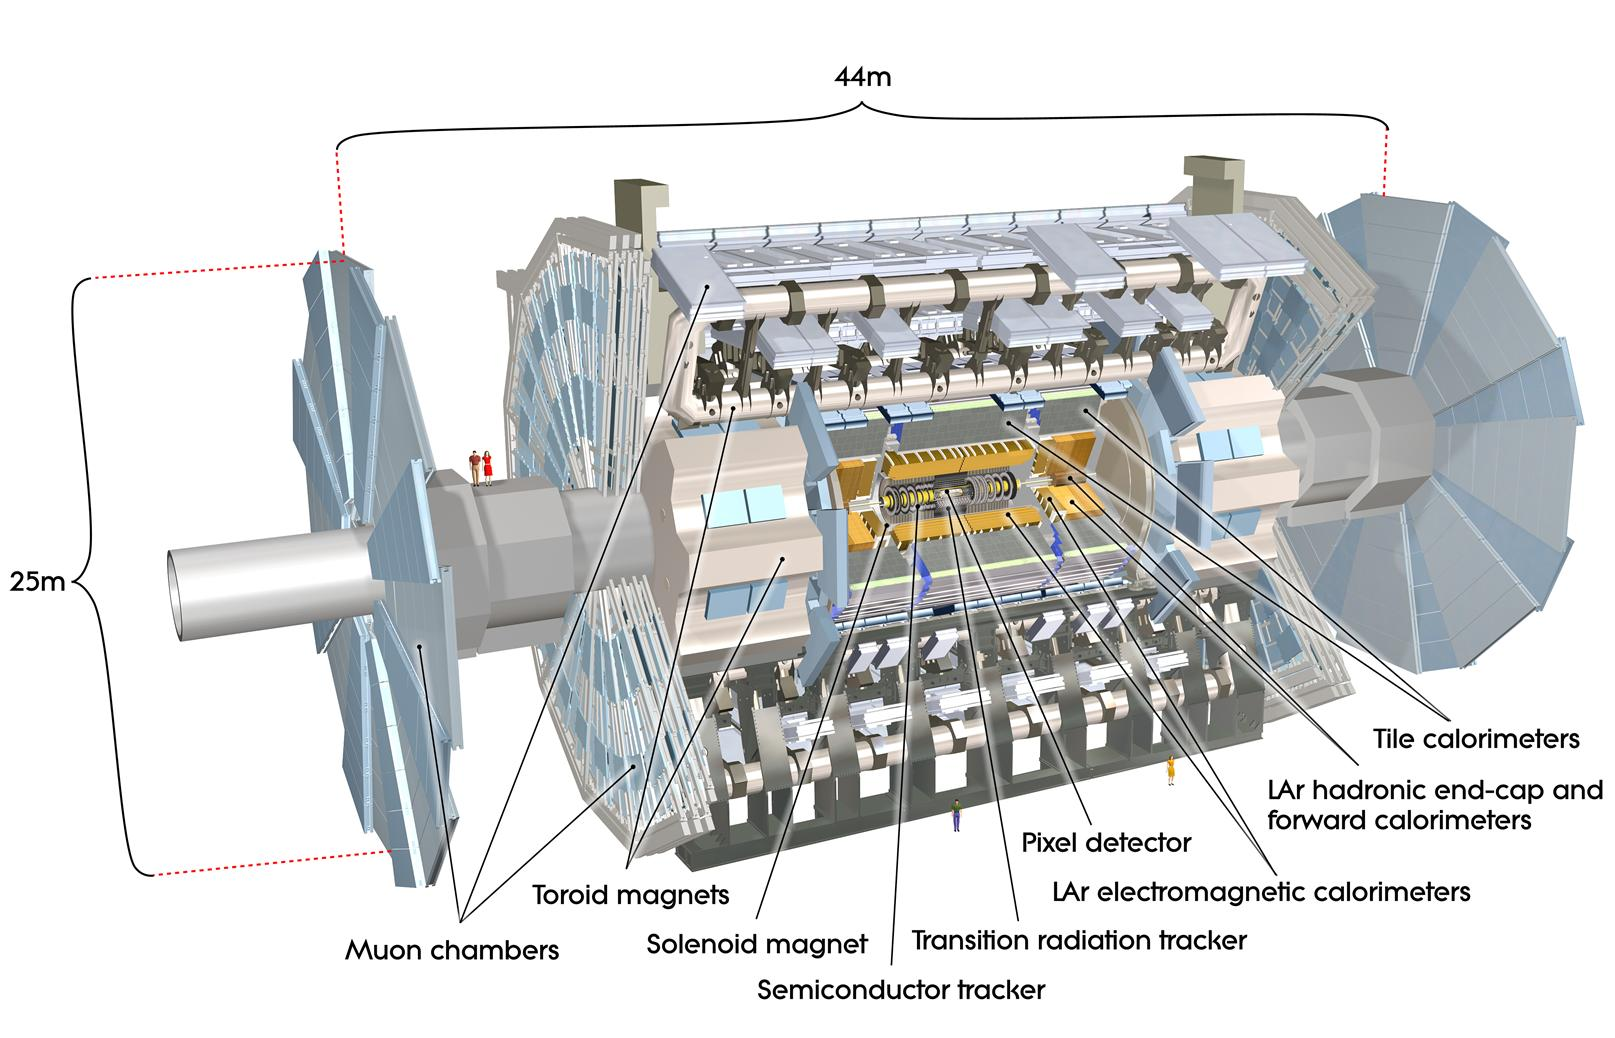
\includegraphics[width=.95\linewidth]{figs/chapter_detector/ATLAS_detector.jpg}
\caption{Cut-away view of the ATLAS detector. The dimensions of the detector are 25 m in height and 44 m in length. The overall weight of the detector is approximately 7000 tonnes.}
\label{fig:detector_ATLAS_detector}
\end{figure}



\subsubsection{Inner Detector}

The ATLAS Inner Detector (ID)~\cite{Aad:2008zzm} is designed to provide hermetic and robust pattern recognition, excellent momentum resolution and both primary and secondary vertex measurements for charged tracks above a given $\pT$ threshold (nominally 0.5 GeV, but can go as low as 0.1 GeV in some cases) and within the pseudorapidity range $|\eta|<2.5$. The ID layout, as shown in Figure~\ref{fig:detector_ATLAS_ID}, reflects the performance requirements. The ID is contained within a cylindrical envelope of 7 m and of radius 1.2 m, within a solenoidal magnetic field of 2 T.

\begin{figure}[H]
\centering
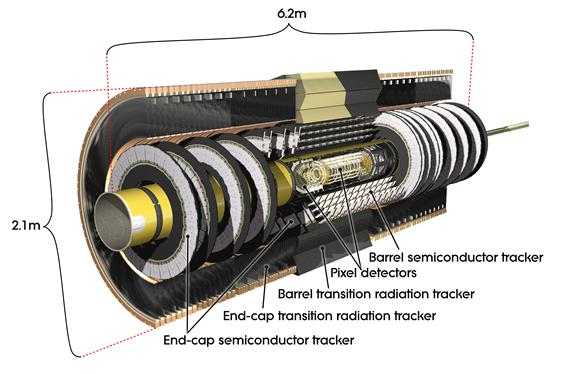
\includegraphics[width=.95\linewidth]{figs/chapter_detector/ATLAS_ID.jpg}
\caption{Cut-away view of the ATLAS Inner Detector. The ID is contained within a cylindrical envelope of length 7 m and of radius 1.2 m, within a solenoidal magnetic field of 2 T.}
\label{fig:detector_ATLAS_ID}
\end{figure}

The ID consists of three independent but complementary sub-detectors. At inner radii, high-resolution pattern recognition capabilities are available using discrete space-points from silicon Pixel layers and stereo pairs of silicon micro-strip (SCT) layers. At large radii, the transition radiation tracker (TRT) comprises many layers of gaseous straw tube elements interleaved with transition radiation material. Pixel, SCT and TRT sub-detectors will be described below separately.



\paragraph{Pixel}

The pixel~\cite{Aad:2008zz} detector is the innermost element of the Inner Detector as shown in Figure~\ref{fig:detector_ATLAS_ID}. The pixel tracker is designed to provide at least three points on a charged track emanating from the collision region. The principle components of the pixel tracking system are the following:
\begin{itemize}
\item The active region of the pixel detector, which is composed of three barrel layers and a total of six disk layers, three at each end of the barrel region;
\item Internal services and their associated mechanical support structures on both ends of the active detector region;
\item A pixel support tube into which the active part of the pixel detector and the services and related support structures are inserted and located;
\item External services that are connected to the internal services at the end of the pixel support tube.
\end{itemize}

The active region of the pixel detector is shown in a schematic view in Figure~\ref{fig:detector_ATLAS_ID_pixel}. The active part of the pixel system consists of three barrel layers: Layer 0, Layer 1 and Layer 2, and two identical endcap regions, each with three disk layers. The basic building block of the active part of the pixel detector is a module that is composed of silicon sensors, front-end electronics and flex-hybrids with control circuits. All modules are functionally identical at the sensor/integrated circuit level, but different somewhat in the interconnection schemes for barrel modules and disk modules. The nominal pixel size is 50 microns in the $\phi$ direction and 400 microns in $z$ (beam axis) and $r$ (disk region). There are 46080 pixel electronics channels in a module. The total number of pixels in the system approximately 67 million in the barrel and 13 million in the endcaps, covering a total area of about 1.7 $\text{m}^2$.

\begin{figure}[H]
\centering
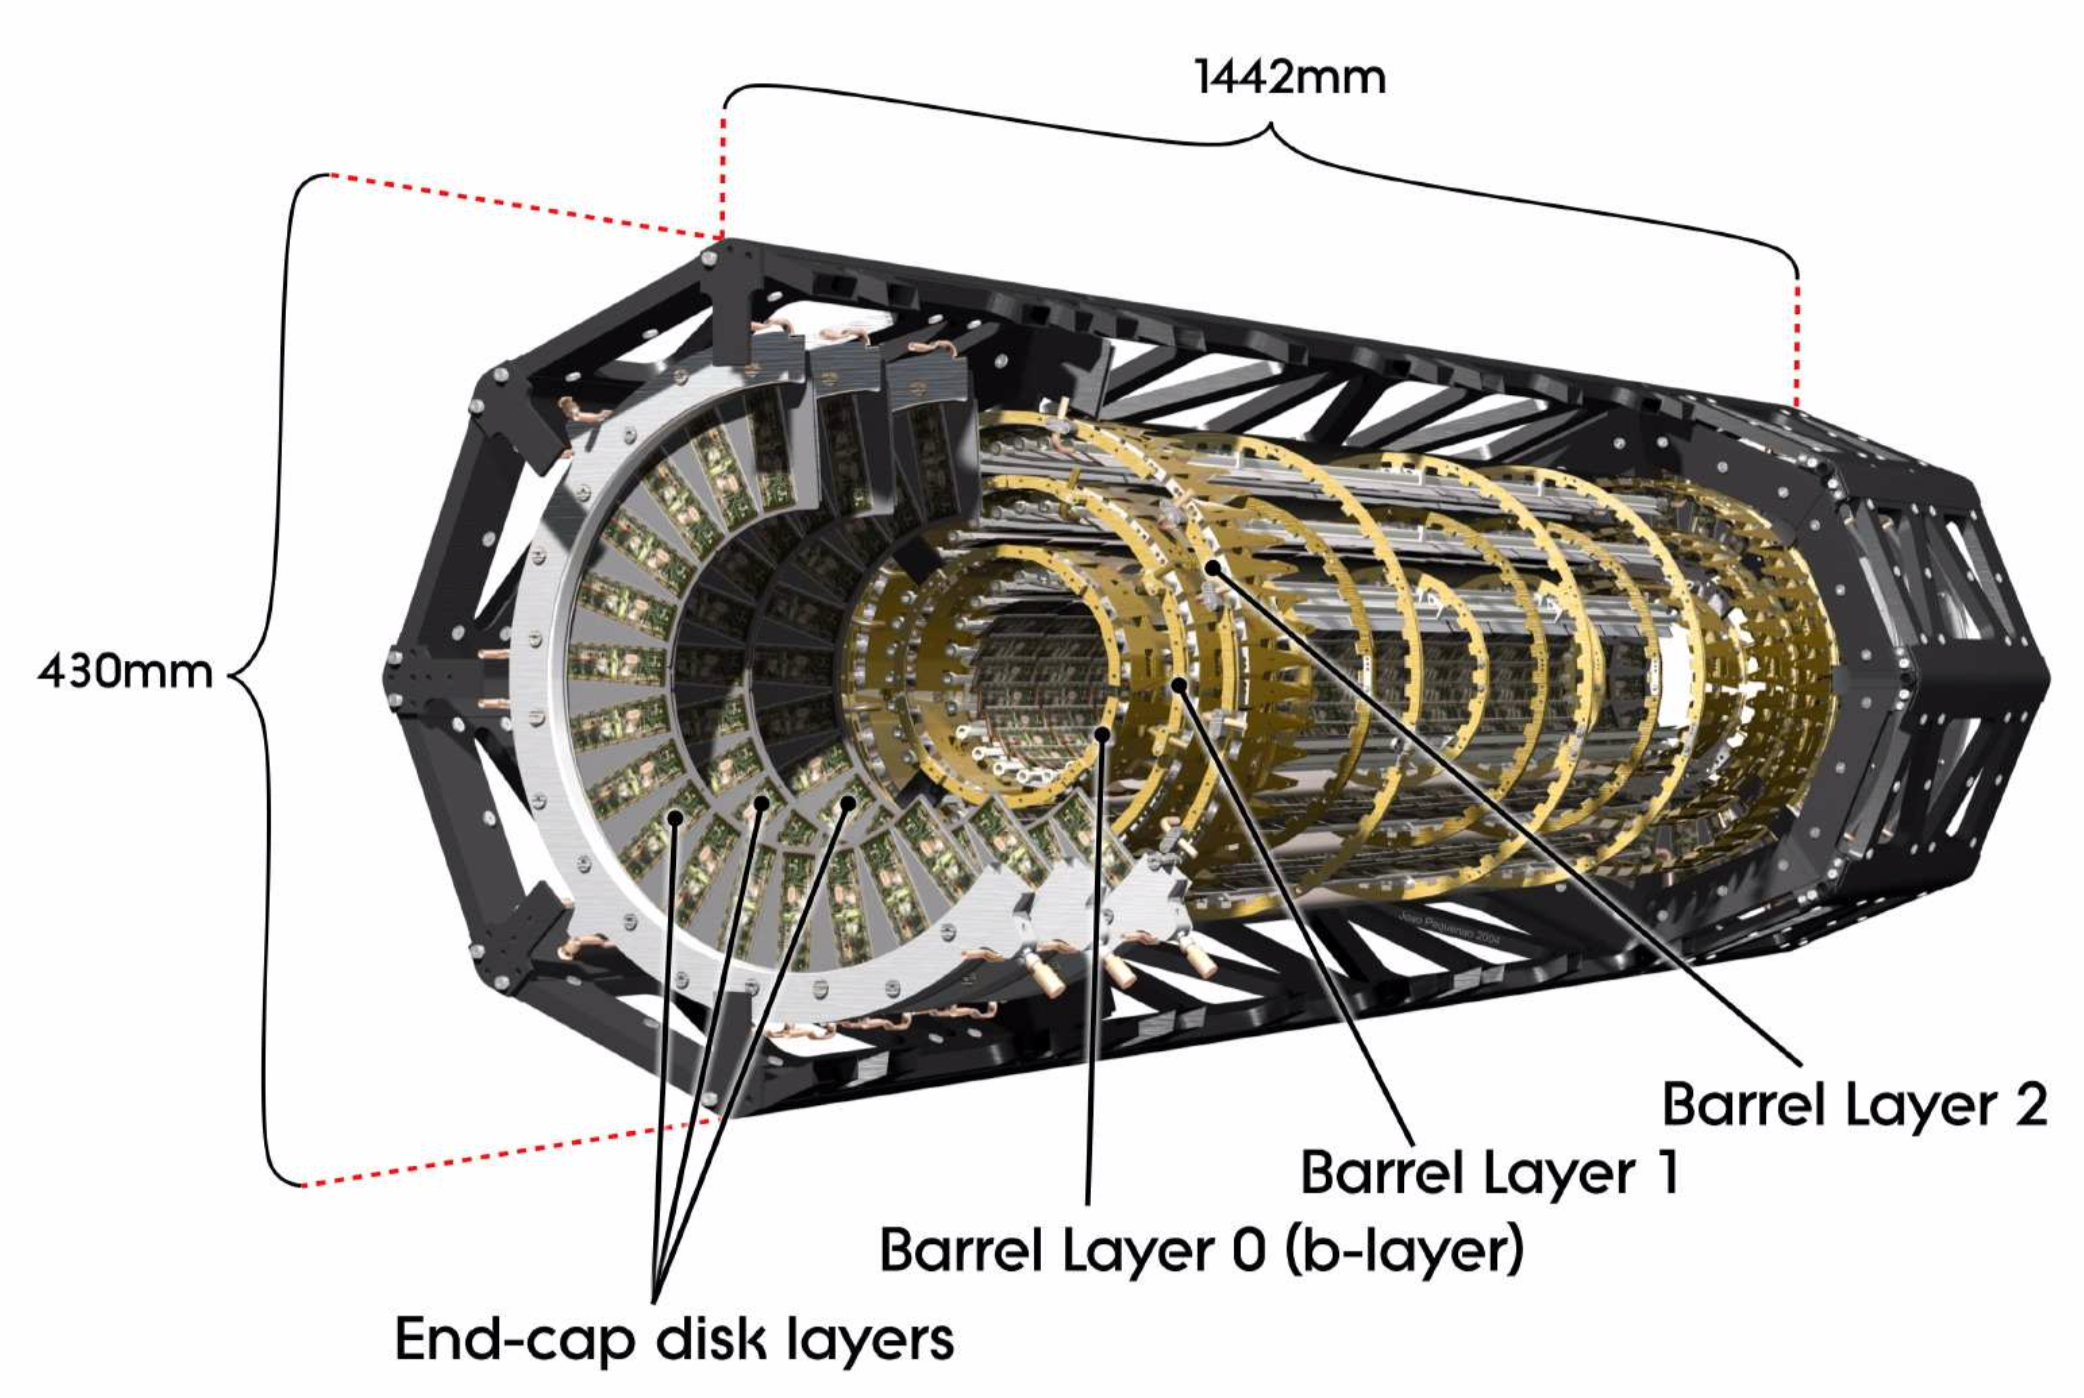
\includegraphics[width=.95\linewidth]{figs/chapter_detector/ATLAS_ID_pixel.png}
\caption{A schematic view of the active region of the pixel detector consisting of barrel and endcap layers.}
\label{fig:detector_ATLAS_ID_pixel}
\end{figure}

To get an idea of the number of pixel hits in different region, left panel of Figure~\ref{fig:detector_ATLAS_ID_pixel_hits} shows an average number of pixel hits per track as a function of pseudorapidity $\eta$. For $|\eta|<2.0$, the average pixel hits is around four, instead of three, which corresponds to the three barrel layers discussed above. This is because an additional pixel layer, the insertable B-layer (IBL), was installed between Run 1 (2010-2013) and Run 2 (2015-2018). This additional layer further increases the performance of tracking reconstruction. For $2.0<|\eta|<2.5$, the average pixel hits is larger, due to the additional endcap layers. The right panel of Figure~\ref{fig:detector_ATLAS_ID_pixel_hits} shows the distribution of number of pixel hits per track. It suggests that most tracks go through all the four barrel layers, while very few tracks could have pixel hits up to 7. The consistency between 2017 and 2015 means that the performance of pixel sub-detector is stable during the Run 2.

\begin{figure}[H]
\centering
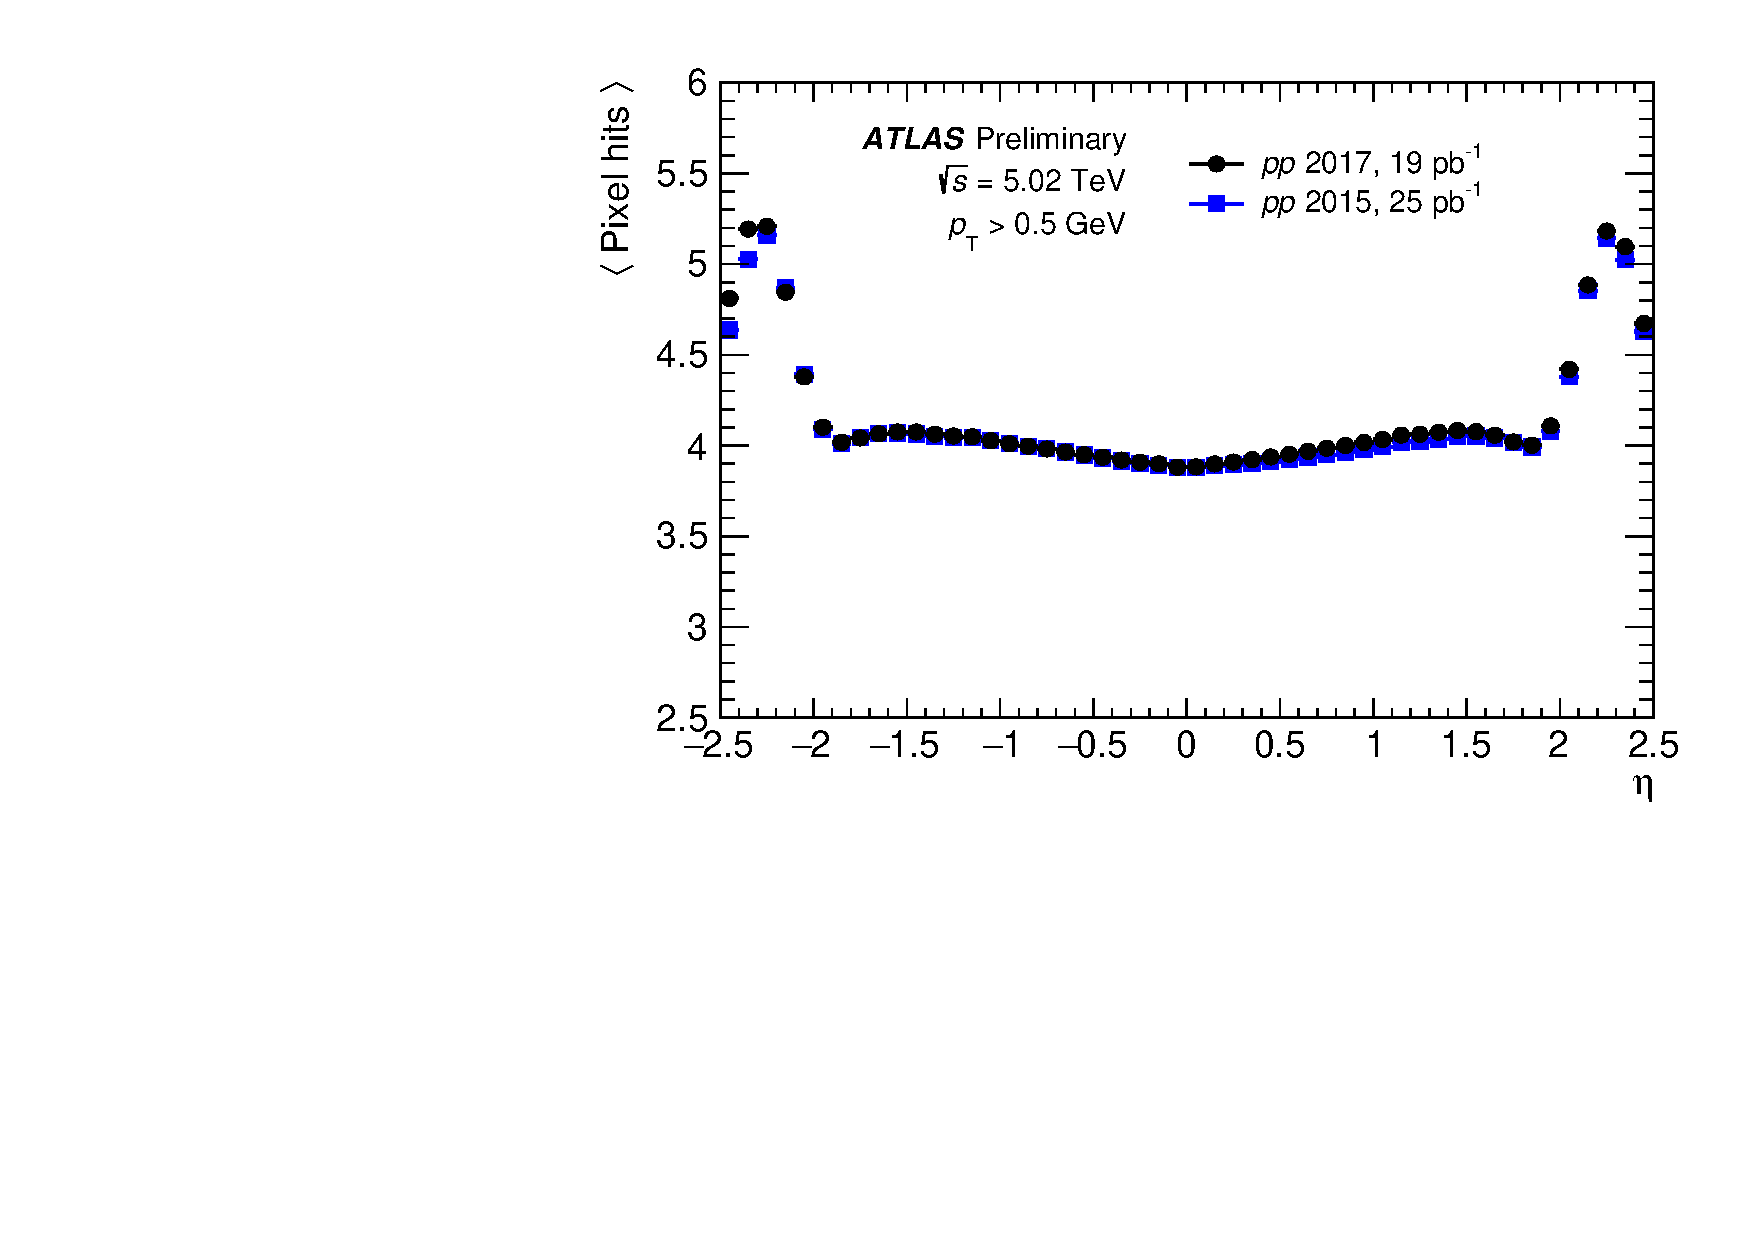
\includegraphics[width=.475\linewidth]{figs/chapter_detector/ATLAS_ID_pixel_hits1.pdf}
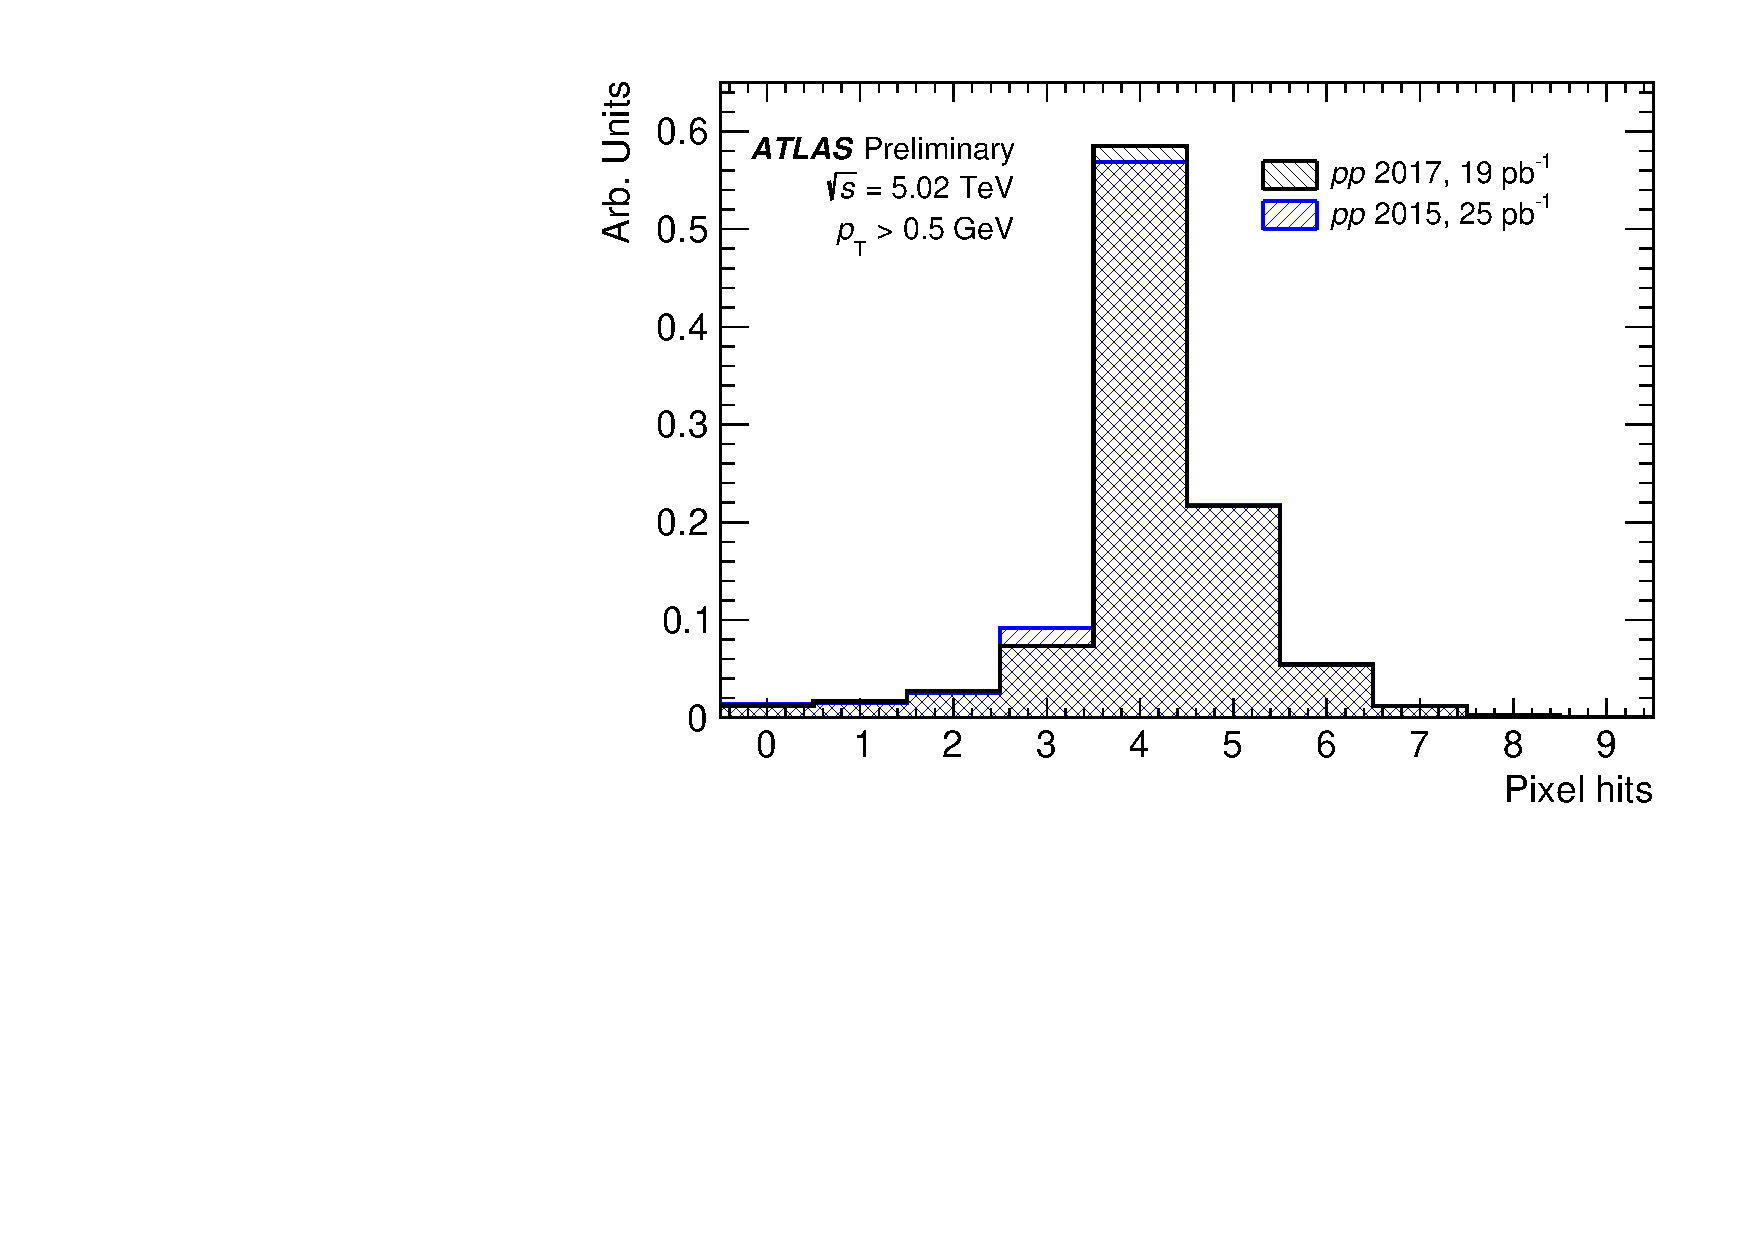
\includegraphics[width=.475\linewidth]{figs/chapter_detector/ATLAS_ID_pixel_hits2.pdf}
\caption{Left: an average number of pixel hits per track as a function of pseudorapidity. Right: a number of pixel hits per track. Tracks are required to have $\pT>0.5$ GeV. Events are required to have a reconstructed vertex.}
\label{fig:detector_ATLAS_ID_pixel_hits}
\end{figure}



\paragraph{SCT}

The SemiConductor Tracker (SCT)~\cite{Ahmad:2007zza} surround the pixel detector, and uses semiconductor technology to provide precision space-point coordinates. In the SCT there are four cylinders in the barrel and nine disks in each of the two endcaps, with every layer able to read out a position in two dimensions. There are in total 8448 identical rectangular single-sided $p$-in-$n$ sensors installed in the ATLAS barrel SCT and 6944 single-sided $p$-in-$n$ sensors, of five different wedge-shaped geometries, in the SCT endcaps. The micro strip sensors are assembled as part of barrel and endcap detection modules in the SCT. In most cases there are two single-sided sensors on each side of a module, glued back-to-back around a high thermal conductivity substrate. The sensor strips are AC-coupled to binary readout electronics, with the ABCD3TA custom ASIC~\cite{Campabadal:2005rj} providing the front-end amplification, discrimination, pipeline, de-randomisation and data compression functions. The layout of the barrel sensors within an SCT module is shown in Figure~\ref{fig:detector_ATLAS_ID_SCT}, together with modules mounted on a barrel.

\begin{figure}[H]
\centering
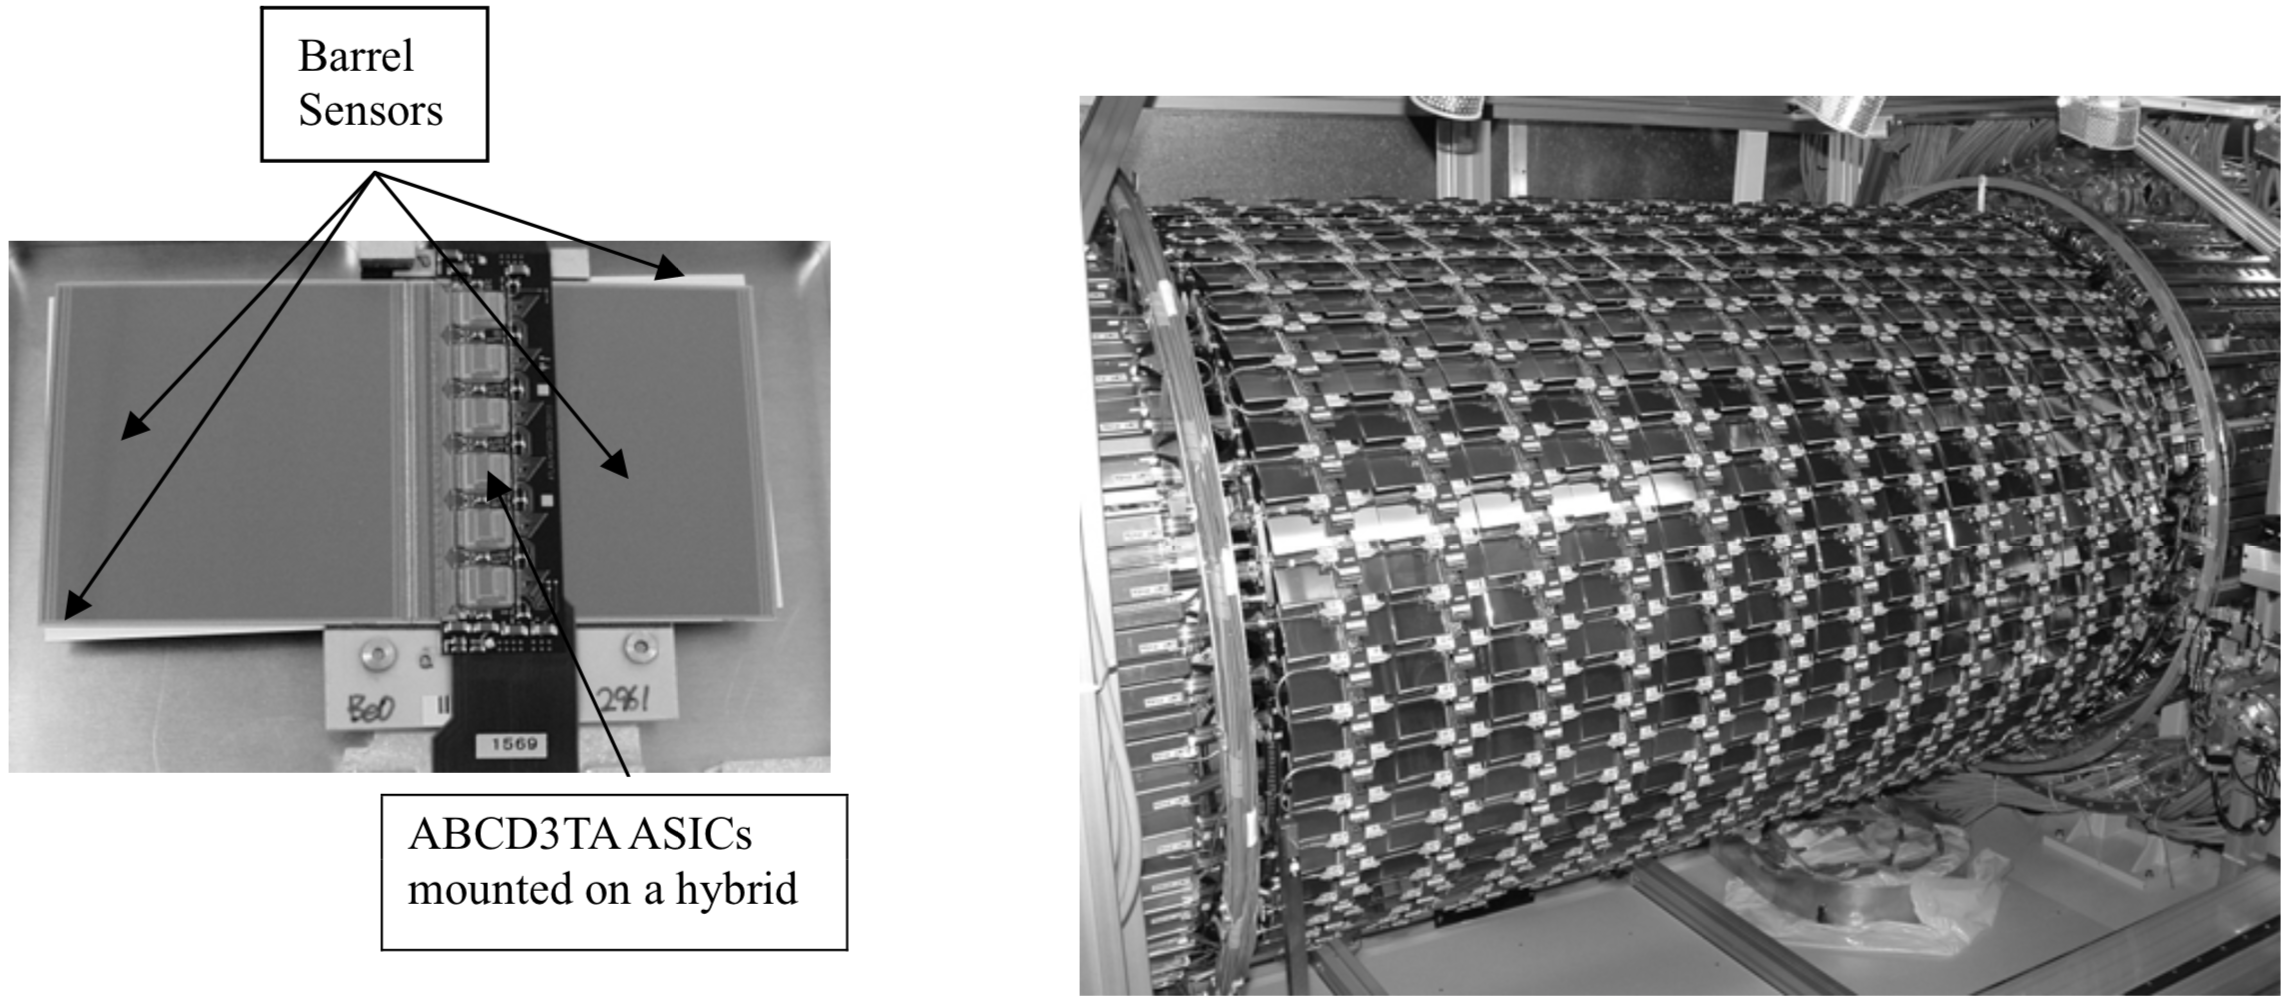
\includegraphics[width=.95\linewidth]{figs/chapter_detector/ATLAS_ID_SCT.png}
\caption{Left: Layout of the 4 sensors (2 on the upper surface, 2 on the lower surface, with 40 mrad stereo rotation) in the SCT barrel module. The readout ASICs are mounted on a hybrid, bridged over the sensors. Right: Modules mounted on the outermost of the 4 barrel structures of the ATLAS SCT.}
\label{fig:detector_ATLAS_ID_SCT}
\end{figure}

To get an idea of the number of hits per track in different regions of the SCT detector, left panel of Figure~\ref{fig:detector_ATLAS_ID_SCT_hits} shows an average number of SCT hits as a function of pseudorapidity $\eta$. For $|\eta|<1.5$, the average SCT hits is around 8, which corresponds to the four cylinders (2 sensors on each side) in the barrel region. For $1.5<|\eta|<2.5$, the average SCT hits is larger, due to additional 9 endcap disks. The right panel of Figure~\ref{fig:detector_ATLAS_ID_SCT_hits} shows the distribution of number of SCT hits per track. The number of hits for most track is between 8 and 10. The consistency between 2017 and 2015 indicates that the performance of SCT is stable during the Run 2.

\begin{figure}[H]
\centering
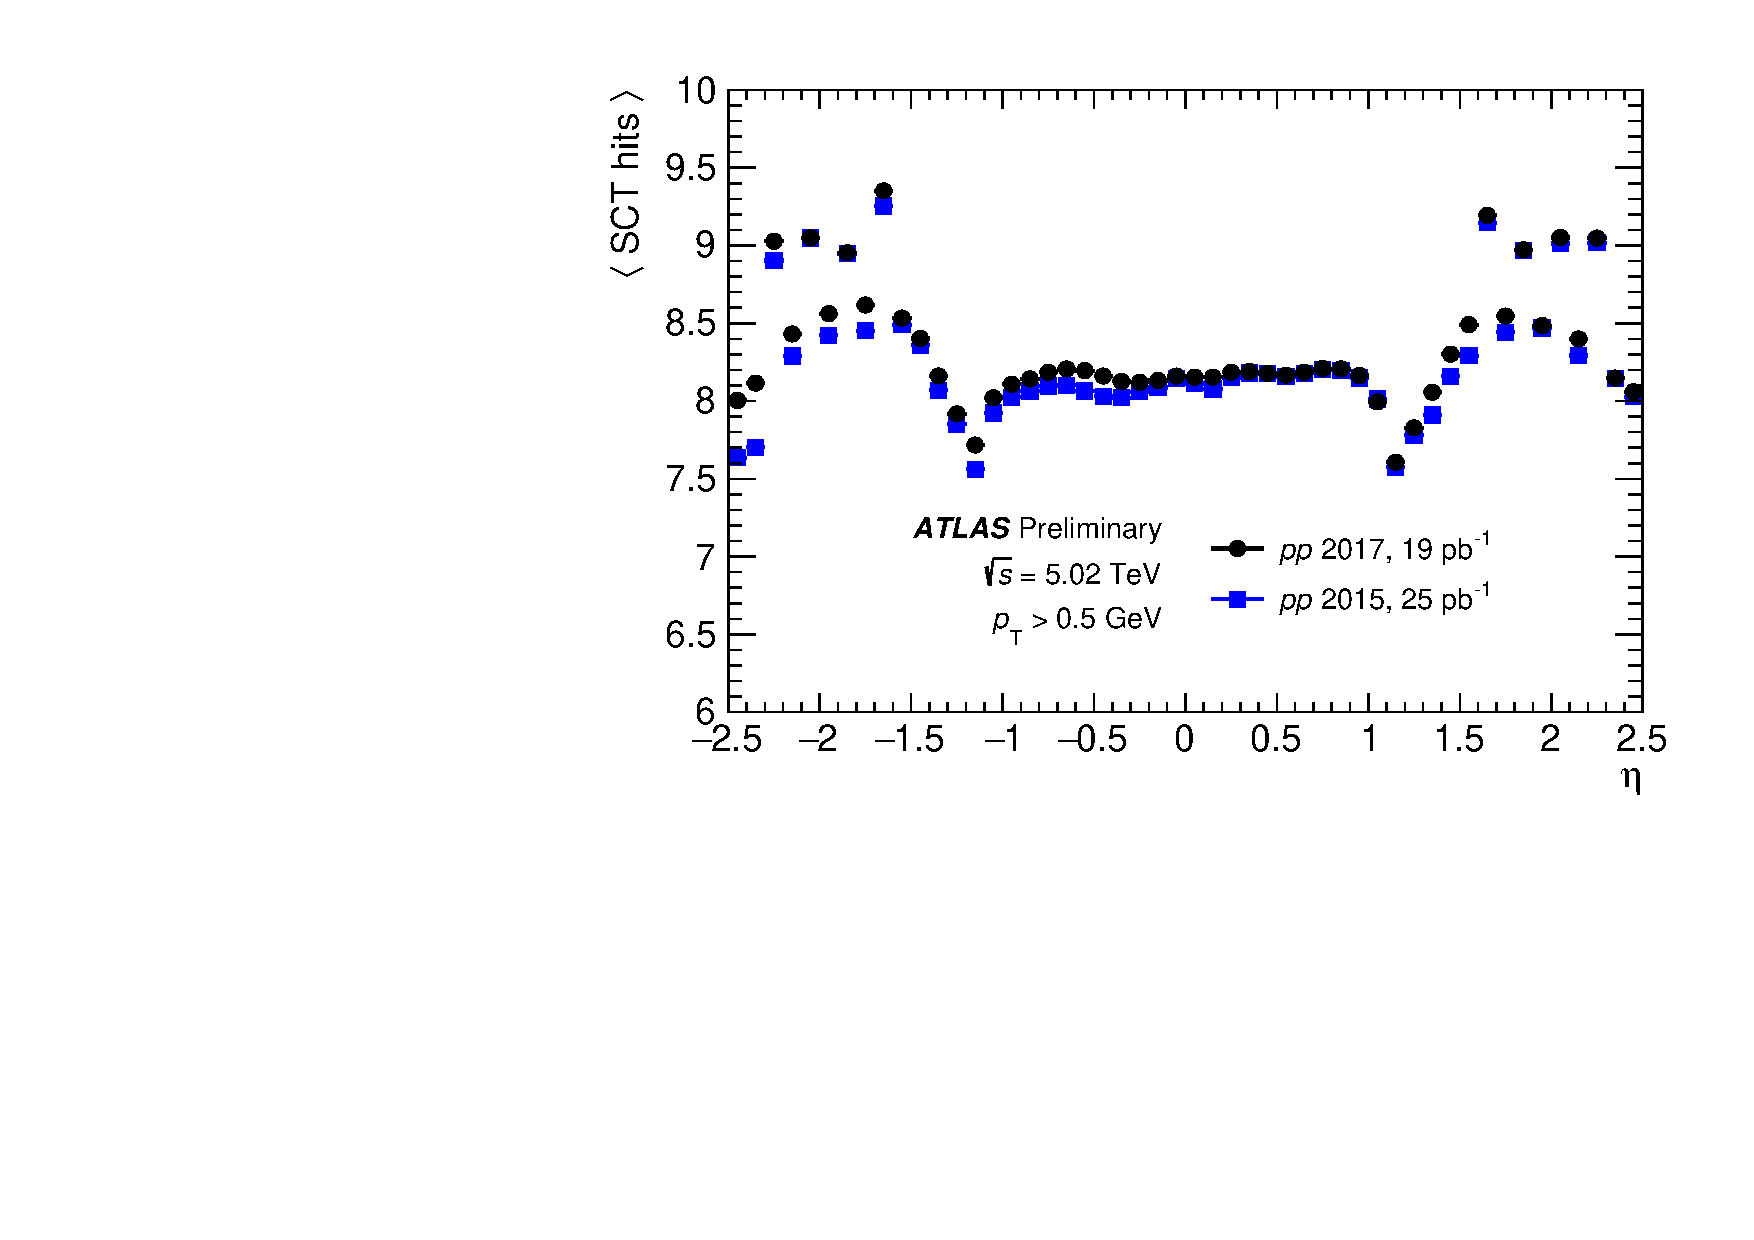
\includegraphics[width=.475\linewidth]{figs/chapter_detector/ATLAS_ID_SCT_hits1.pdf}
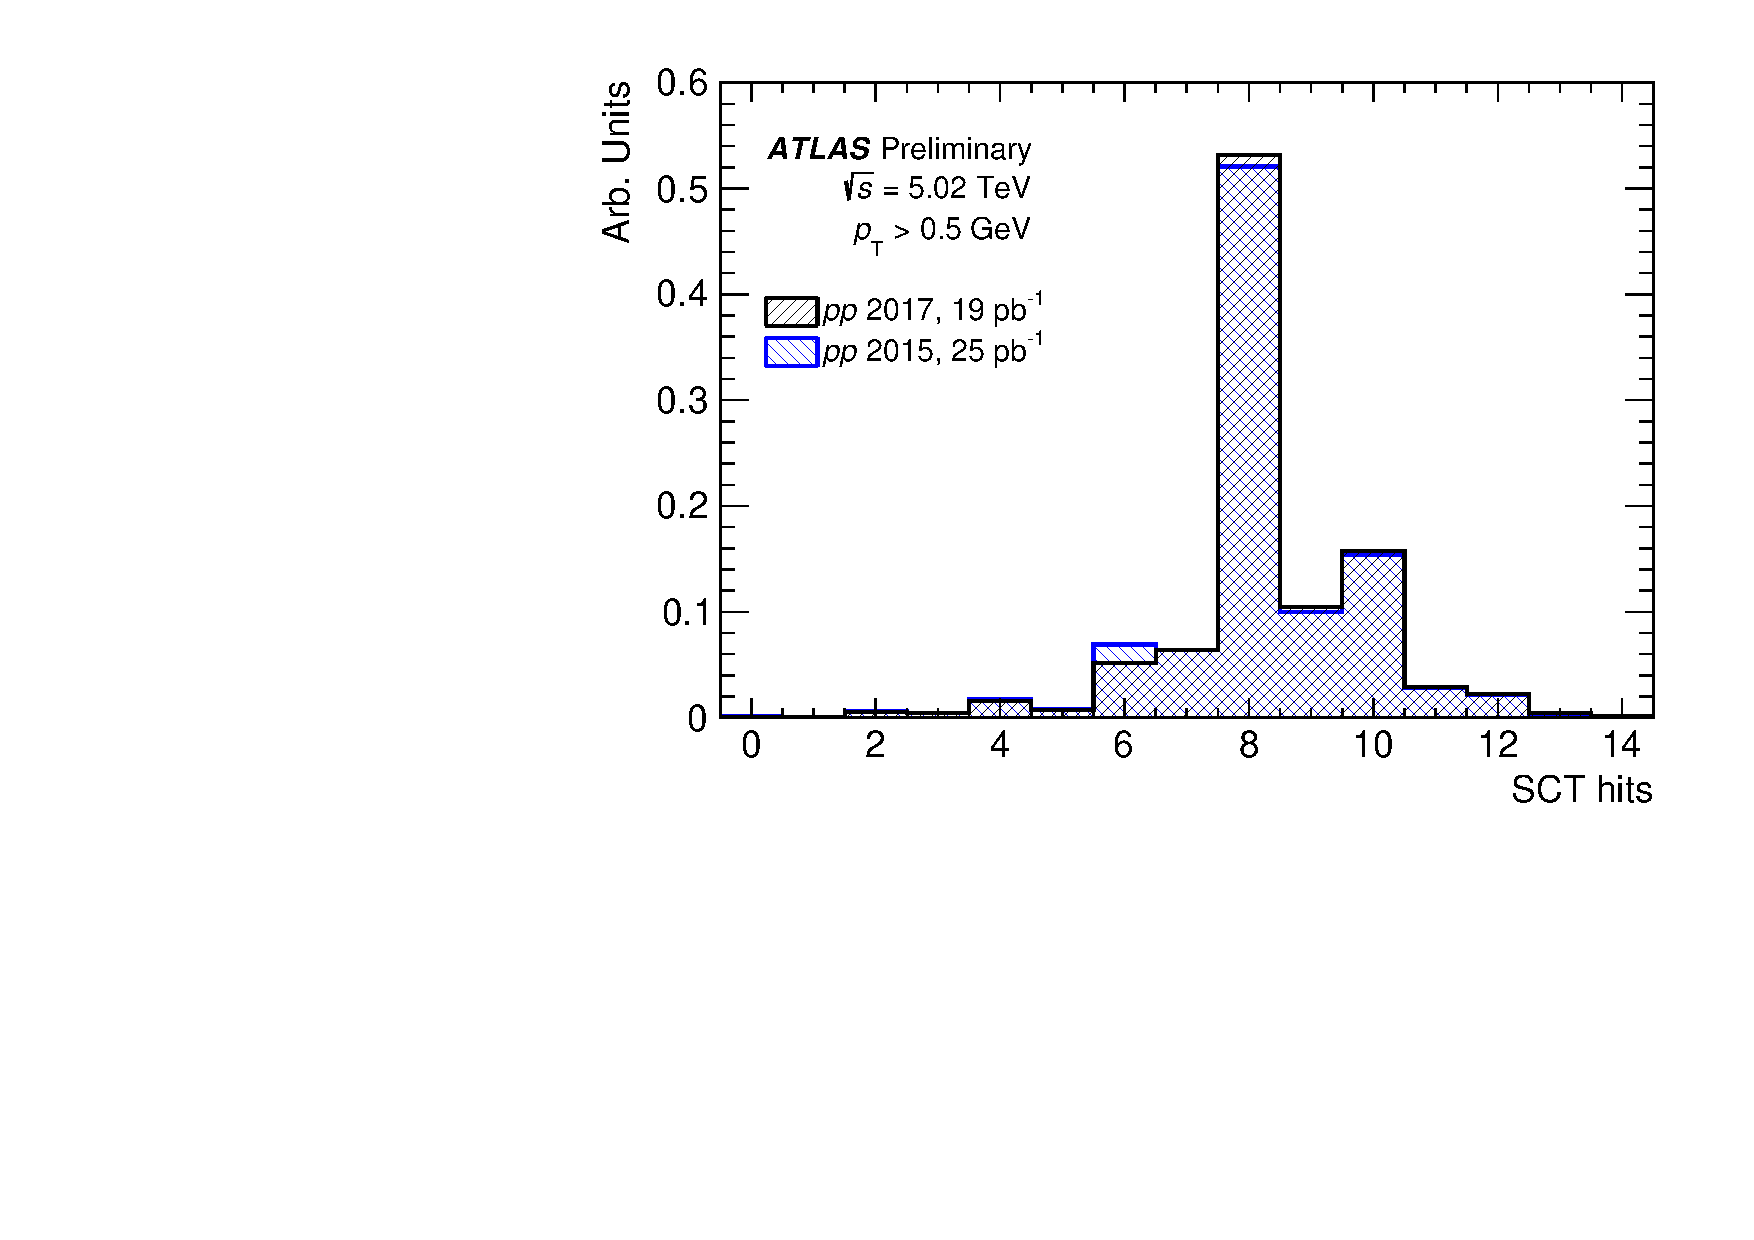
\includegraphics[width=.475\linewidth]{figs/chapter_detector/ATLAS_ID_SCT_hits2.pdf}
\caption{Left: an average number of SCT hits per track as a function of pseudorapidity. Right: a number of SCT hits per track. Tracks are required to have $\pT>0.5$ GeV. Events are required to have a reconstructed vertex.}
\label{fig:detector_ATLAS_ID_SCT_hits}
\end{figure}



\paragraph{TRT}

The Transition Radiation Tracker (TRT)~\cite{Abat:2008zza} consists of three parts: a barrel and two endcaps. Its basic elements are thin-walled proportional drift tubes, hereafter called straws. Straw tubes were chosen as detecting elements because they offer a high degree of modularity of the detector and because they can be easily integrated into a medium producing transition without compromising the continuous tracking concept. The barrel part is comprised of 52544 straws 144 cm in length oriented parallel to the beam. The two end-caps each contain 122880 straps 37 cm in length radially aligned to the beam axis. The detector geometry guarantees that particles cross 35-40 straws in a pseudorapidity interval from 0 to 2, providing continuous tracking at larger radii of the Inner Detector while enhancing its pattern recognition ability. The TRT was not used in the heavy-ion program due to high occupancy in most central events which limited its use for tracking and electron identification. The analyses presented here do not make use of the TRT hits information.



\subsubsection{Forward Calorimeter}

Calorimeters measure the energy a particle loses as it passes through the detector. It is usually designed to stop entire or absorb most of the particles coming from a collision, forcing them to deposit all of their energy within the detector. Calorimeters typically consist of layers of passive or absorbing high-density material, for example lead, interleaved with layers of an active medium such as solid lead-glass or liquid argon. Electromagnetic calorimeters measure the energy of electrons and photons as they interact with the matter. Hadronic calorimeters sample the energy of hadrons as they interact with atomic nuclei. Calorimeters can stop most known particles except muons and neutrinos.

Complete calorimeter hermeticity is important for many physics studies at the LHC. In order to extend the pseudorapidity coverage up to 4.9 units, ATLAS uses a liquid argon Forward Calorimeter (FCal)~\cite{Artamonov:2008zz} integrated into the endcap cryostat. The ATLAS FCal covers the pseudorapidity range $3.1 < |\eta| < 4.9$. The main challenge in designing the FCal was to ensure that it would function reliably in the extremely hostile environment close to the LHC beams. In order to have some measurement of longitudinal shower environment, the FCal is divided into three sections, as shown in Figure~\ref{fig:detector_ATLAS_FCal}. In all three sections the construction is such that only radiation hard materials are used, and there are no adhesives used in the joints. All three modules use a novel electrode structure. This consists of copper tubes parallel to the beam axis, which contain electrode rods. In the FCal1 the electrode rods and the calorimeter matrix are copper. This serves to ensure a good thermal conductivity close the shower maximum, and avoids local heating, and perhaps boiling of the liquid argon. In order to have an extremely dense detector, the FCal2 and FCal3 modules have tungsten electrode rods, and the matrix consists of small sintered tungsten slugs. The liquid argon gap between the electrode rods, and the copper electrodes tubes is maintained by a spiral of radiation hard PEEK plastic in all three modules.

\begin{figure}[H]
\centering
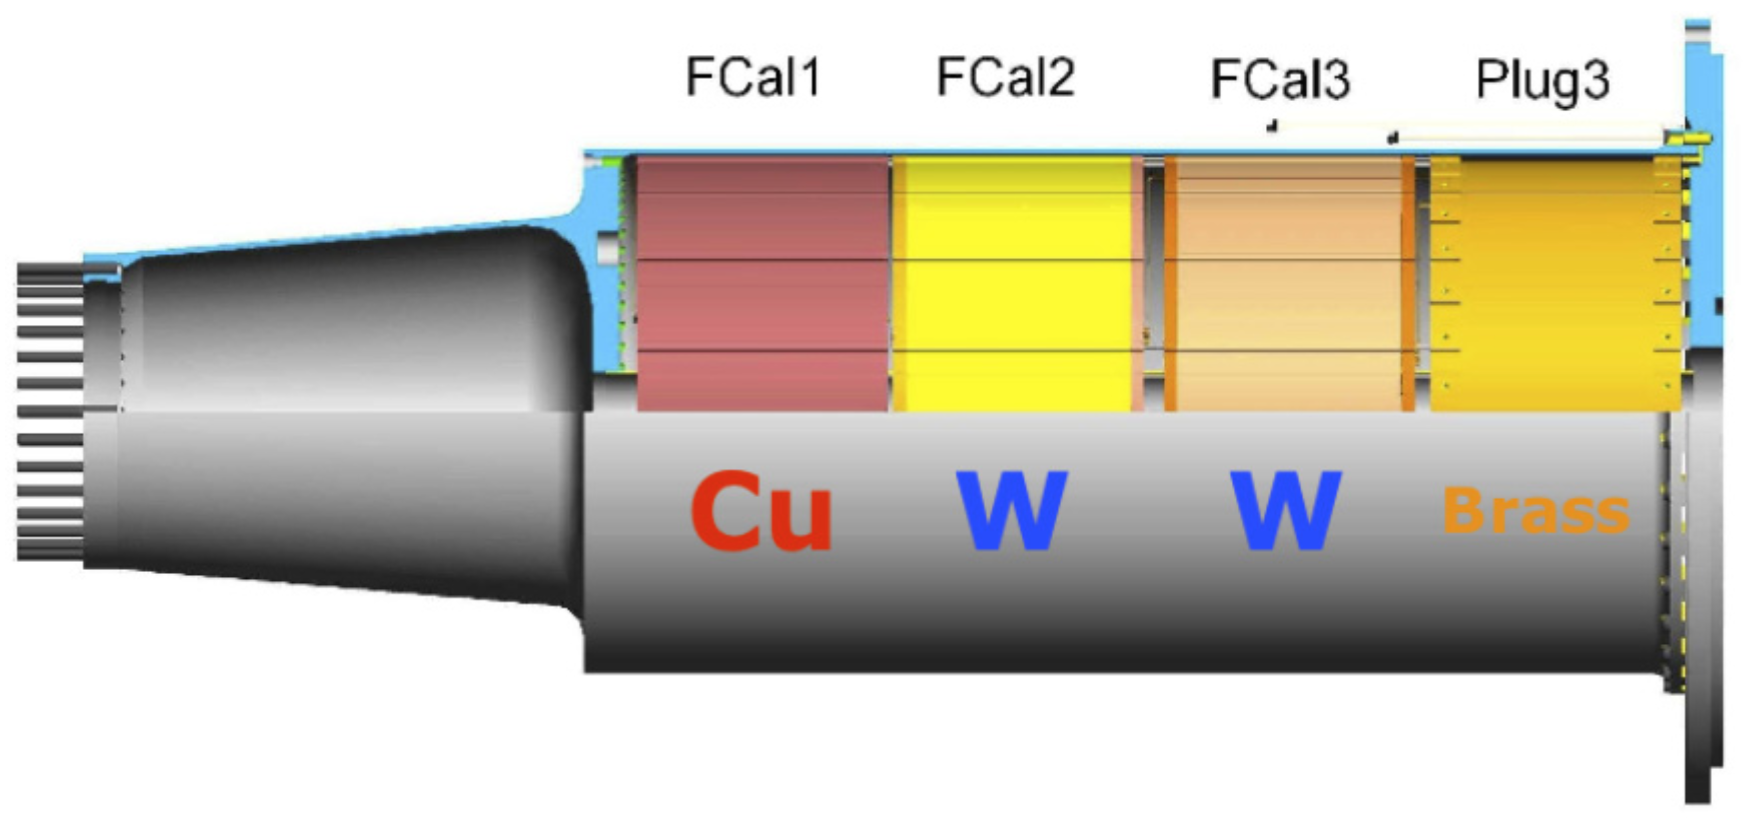
\includegraphics[width=.475\linewidth]{figs/chapter_detector/ATLAS_FCal.png}
\caption{The general arrangement of the FCal, and details of the electrode spacing.}
\label{fig:detector_ATLAS_FCal}
\end{figure}

Left panel of Figure~\ref{fig:detector_ATLAS_FCal_Nch} presents the correlation between number of reconstructed charged particles $\Nchrec$ and total transverse energy in FCal $\Et^\text{FCal}$. A strong correlation is observed. Since in most flow analysis azimuthal angular distribution is measured using charged particles, $\Et^\text{FCal}$ provides an independent observable to quantify the event activities. The determination of centrality using $\Et^\text{FCal}$ will be discussed in Section~\ref{sec:centrality_determination}.

\begin{figure}[H]
\centering
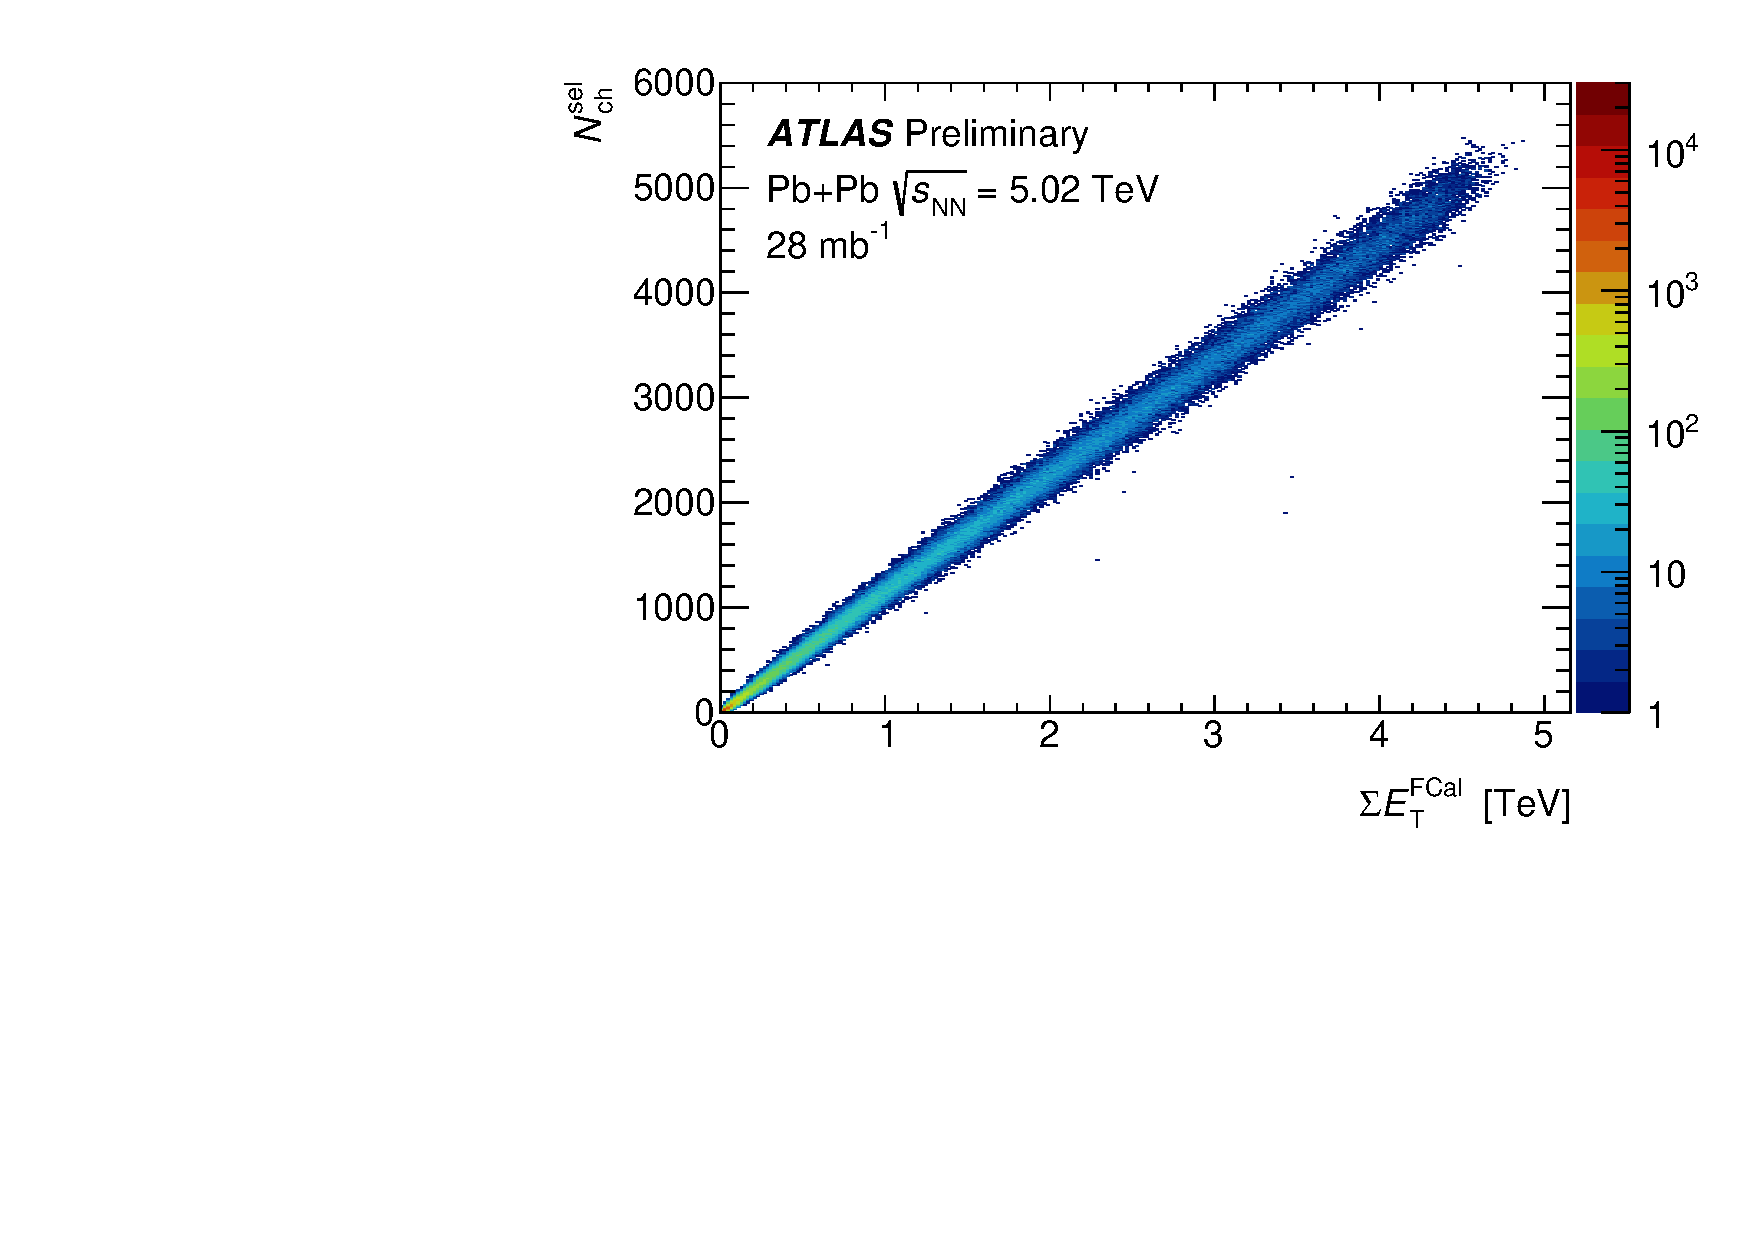
\includegraphics[width=.475\linewidth]{figs/chapter_detector/ATLAS_FCal_Nch.pdf}
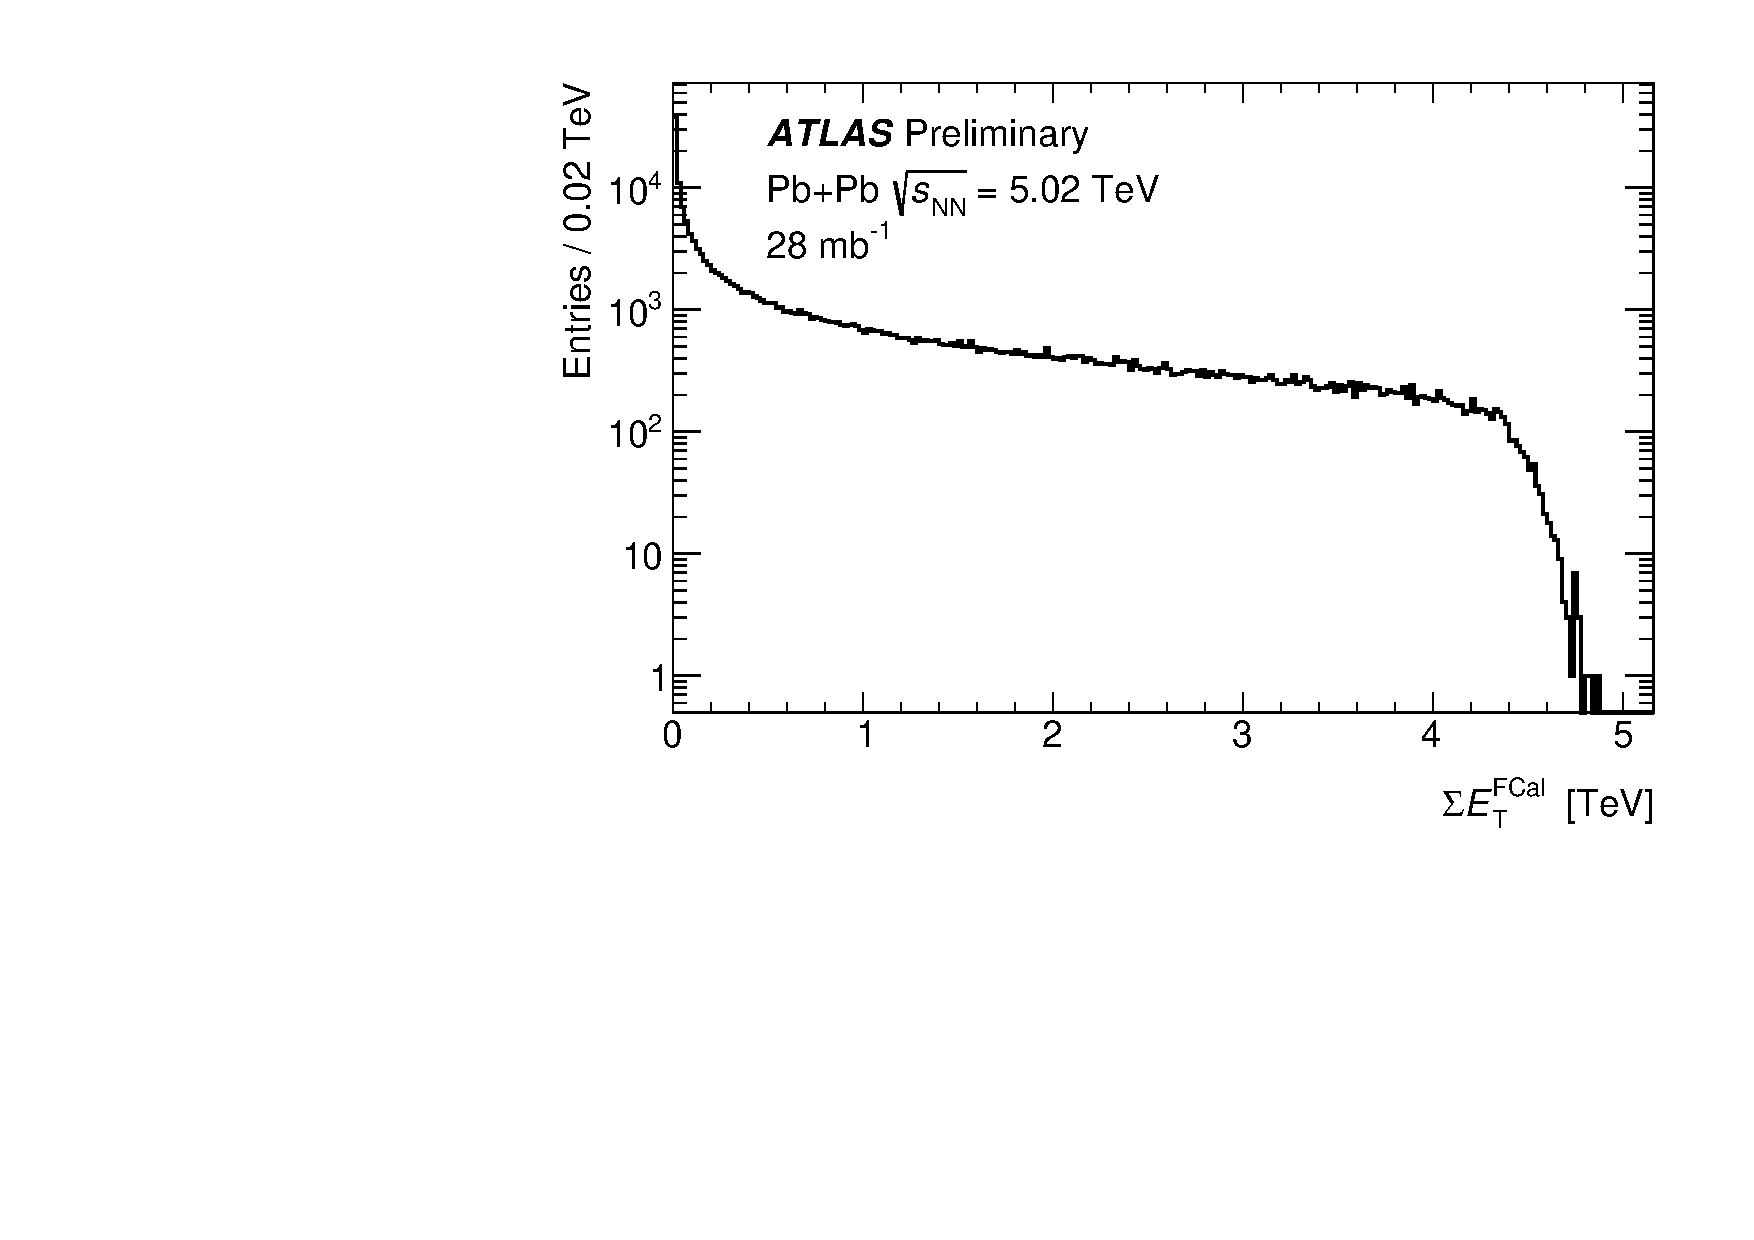
\includegraphics[width=.475\linewidth]{figs/chapter_detector/ATLAS_FCaldis.pdf}
\caption{Left: number of reconstructed charged particle $\Nchrec$, versus total transverse energy $\Et^\text{FCal}$ in the FCal. Tracks are selected from a pseudorapidity range $|\eta|<2.5$ with transverse momentum $\pT>0.3$ GeV. A reconstructed primary vertex is required. Right: distribution of $\Et^\text{FCal}$.}
\label{fig:detector_ATLAS_FCal_Nch}
\end{figure}



\subsubsection{Zero Degree Calorimeter}
\label{sec:zero_degree_calorimeter}

The primary role of Zero Degree Calorimeter (ZDC)~\cite{ATLAS:2007aa} is in event characterization. The ZDC measures the participant number by sampling the spectator neutrons. The ZDC can also measure the orientation of the impact parameter. The secondary role of the ZDC is as a device for luminosity measurement. The ZDC (coincidence) cross-section can be reliably calculated.

The ZDC is located 140 m from the centra of ATLAS on either side, after the beam-pipe splits into two, covering the region $|\eta|>8.3$. It gets its name as it is located along the beam (at zero degrees). Only the neutral particles from the event manage to reach the ZDC as the charged particles are deflected away by the magnetic fields in the beam-pipe. Thus in Pb+Pb collisions the ZDC measures spectator neutrons. Each side of the ZDC consists of four modules as shown in the left bottom panel of Figure~\ref{fig:detector_ATLAS_ZDC}. The detailed design of the modules is shown in the right panel of Figure~\ref{fig:detector_ATLAS_ZDC}. Each module consists of 11 tungsten plates 10 mm thick in the beam direction and steel plates at the front and back (also 10 mm thick). Sandwiched between the plates are 1.5 mm diameter quartz rods that run vertically and are viewed by photomultiplier tubes (PMT) from above, via light-pipes. The quartz rods collect Cherenkov radiation from shower particles and guide them to the PMTs. Each PMT is read out by several channels of a Pre Processor Module (PPM), The PPMs are 64 channel, 40 MHz, 10 bit ADCs. The first two ZDC modules on the C side and the second module on the A side also have quartz rods arranged in an x-y grid along the beam-pipe. These can be used for position measurements of the showers. They were however not used in any of the analyses presented here. 

\begin{figure}[H]
\centering
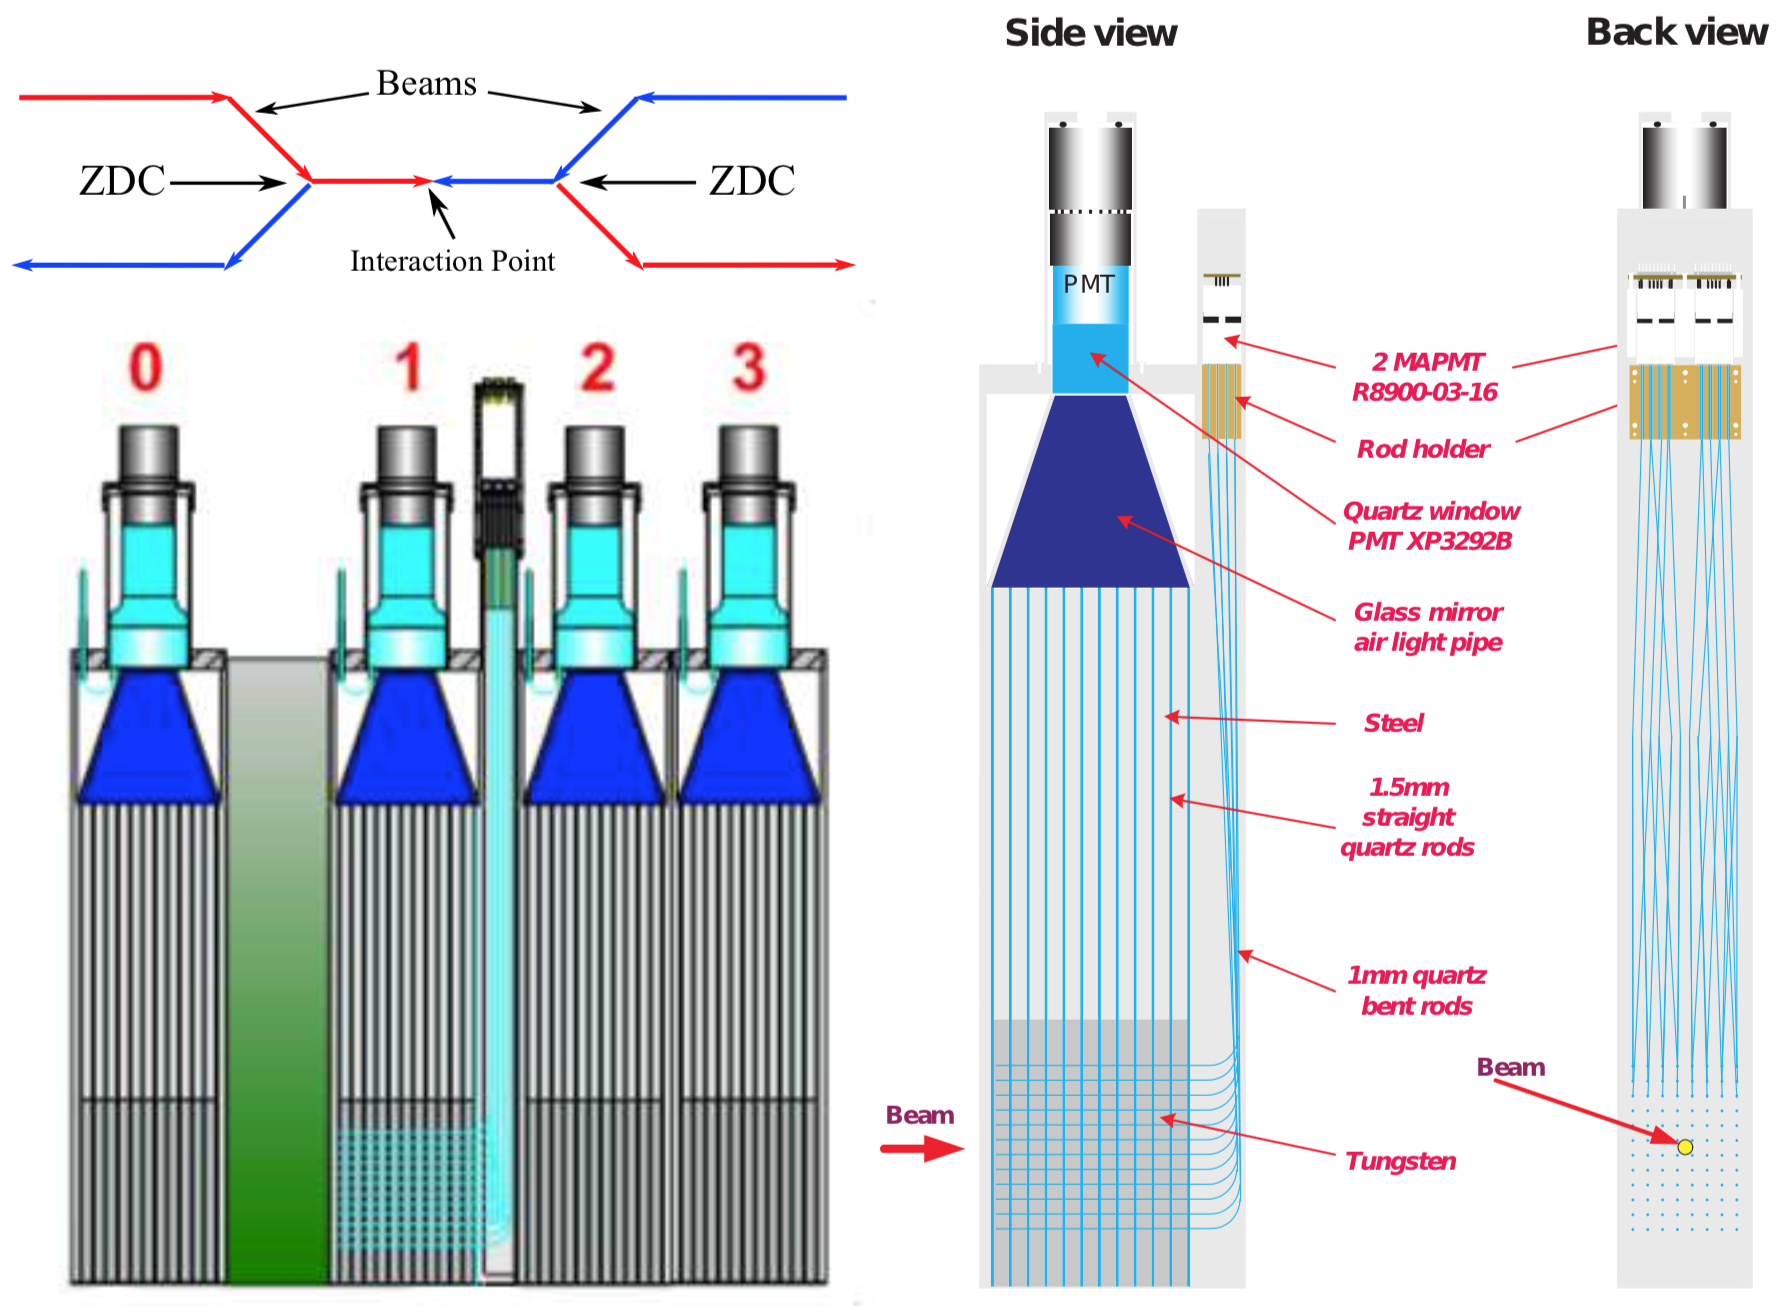
\includegraphics[width=.95\linewidth]{figs/chapter_detector/ATLAS_ZDC.png}
\caption{Left top: the location of the ZDC. Left bottom: the four ZDC modules on the A-side. Right: details of a ZDC module.}
\label{fig:detector_ATLAS_ZDC}
\end{figure}

To get an idea of the energy distribution deposited in ZDC, left panel of Figure~\ref{fig:detector_ATLAS_ZDC_FCal} shows the energy in the ZDC arm C, divided by the most probable energy of the single neutron peak. Peaks showing contributions from up to four neutrons emitted in a single event are clearly visible. Right panel of Figure~\ref{fig:detector_ATLAS_ZDC_FCal} shows the correlation of the sum of the energies in the two ZDC arms, normalized to the single neutron energy, v.s. the sum of transverse energies measured in the FCal. In peripheral collisions ($\Et^\text{FCal}<0.5$ TeV), sum of energies in ZDC and FCal are correlated. While from mid-central to central collisions ($\Et^\text{FCal}>1.0$ TeV), sum of energies in ZDC and FCal are anti-correlated. This is because in these collisions, ZDC mainly measures the energy from spectators, while FCal measures the energy from participants. Numbers of spectators and participants are anti-correlated. The additional events observed beyond the main band of the correlation are mostly pile-up events, i.e. events with more than one reconstructed vertices. This correlation can be used to suppress the fraction of pile-up events (Section~\ref{sec:event_selection}).

\begin{figure}[H]
\centering
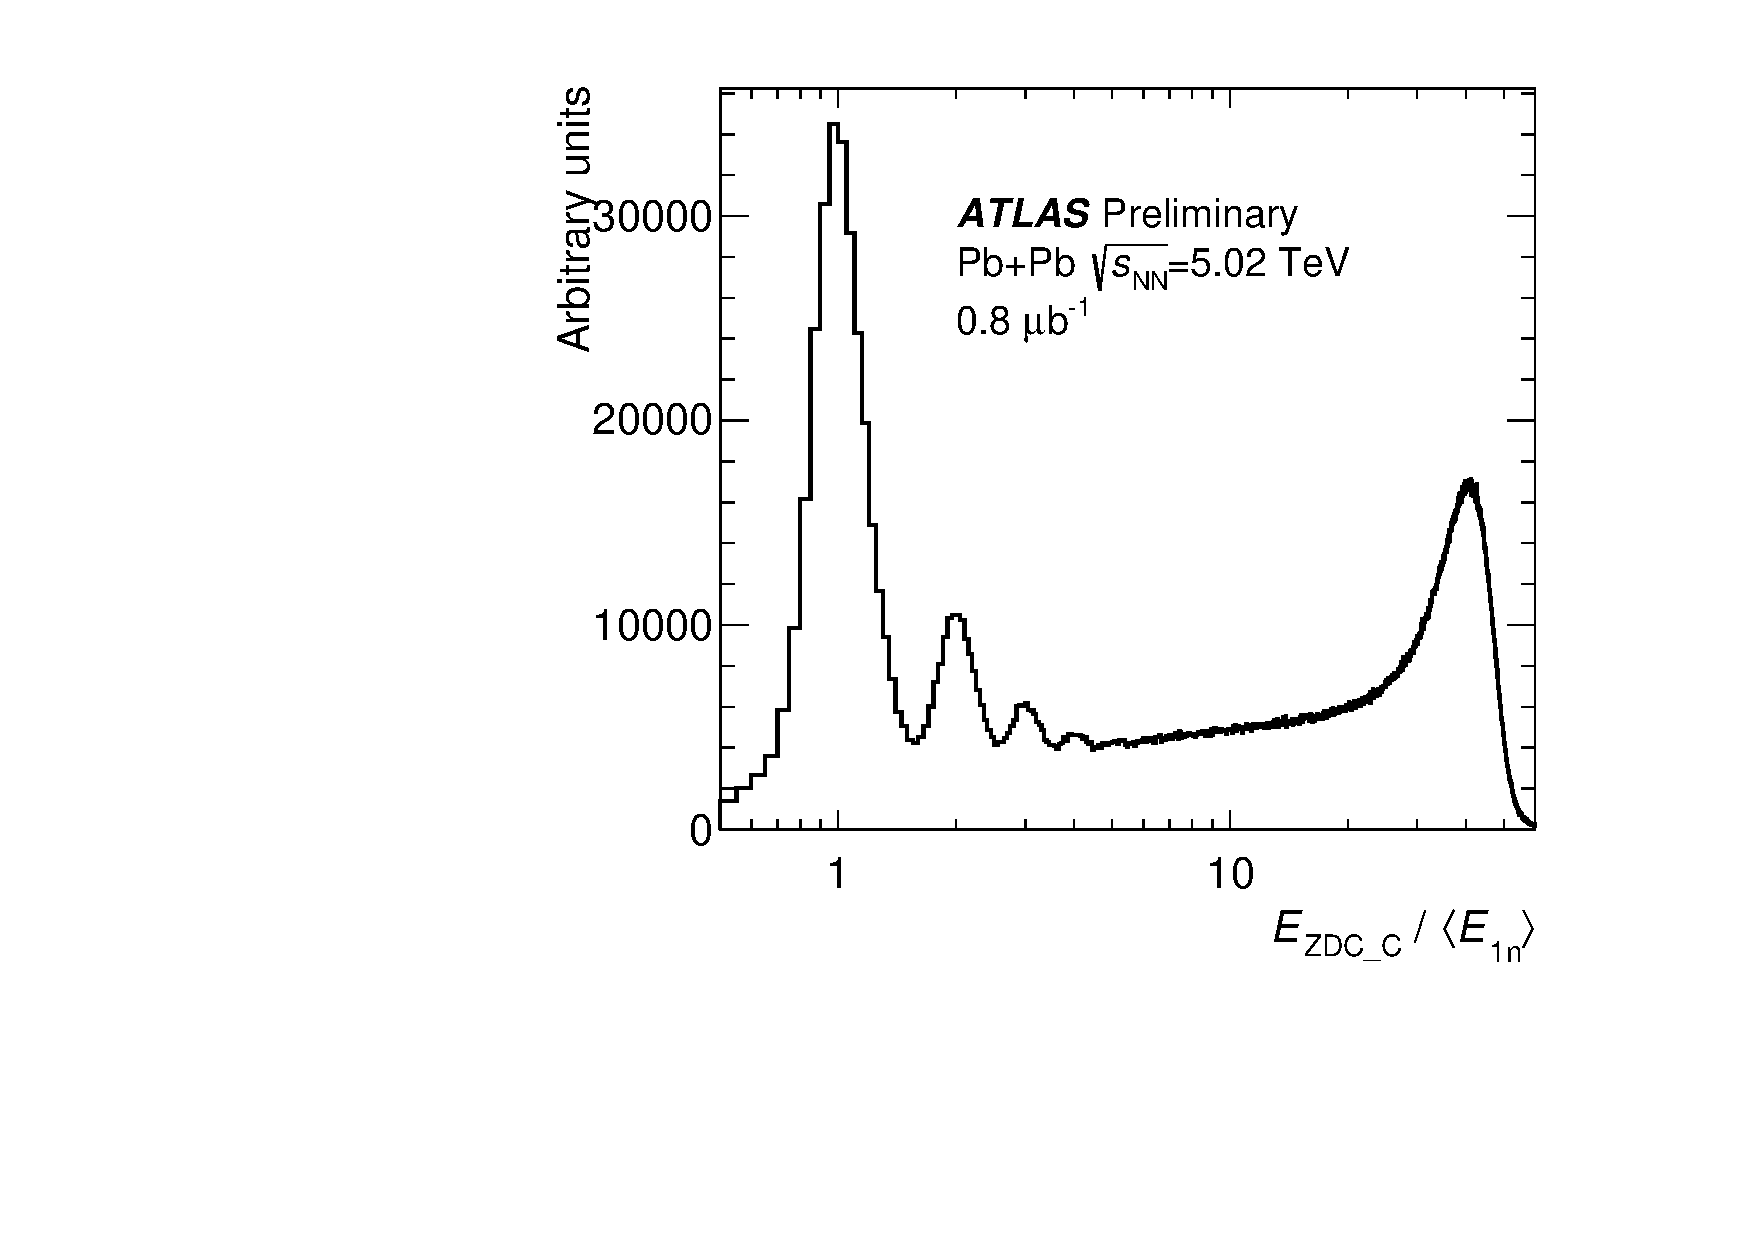
\includegraphics[width=.475\linewidth]{figs/chapter_detector/ATLAS_ZDCdis.pdf}
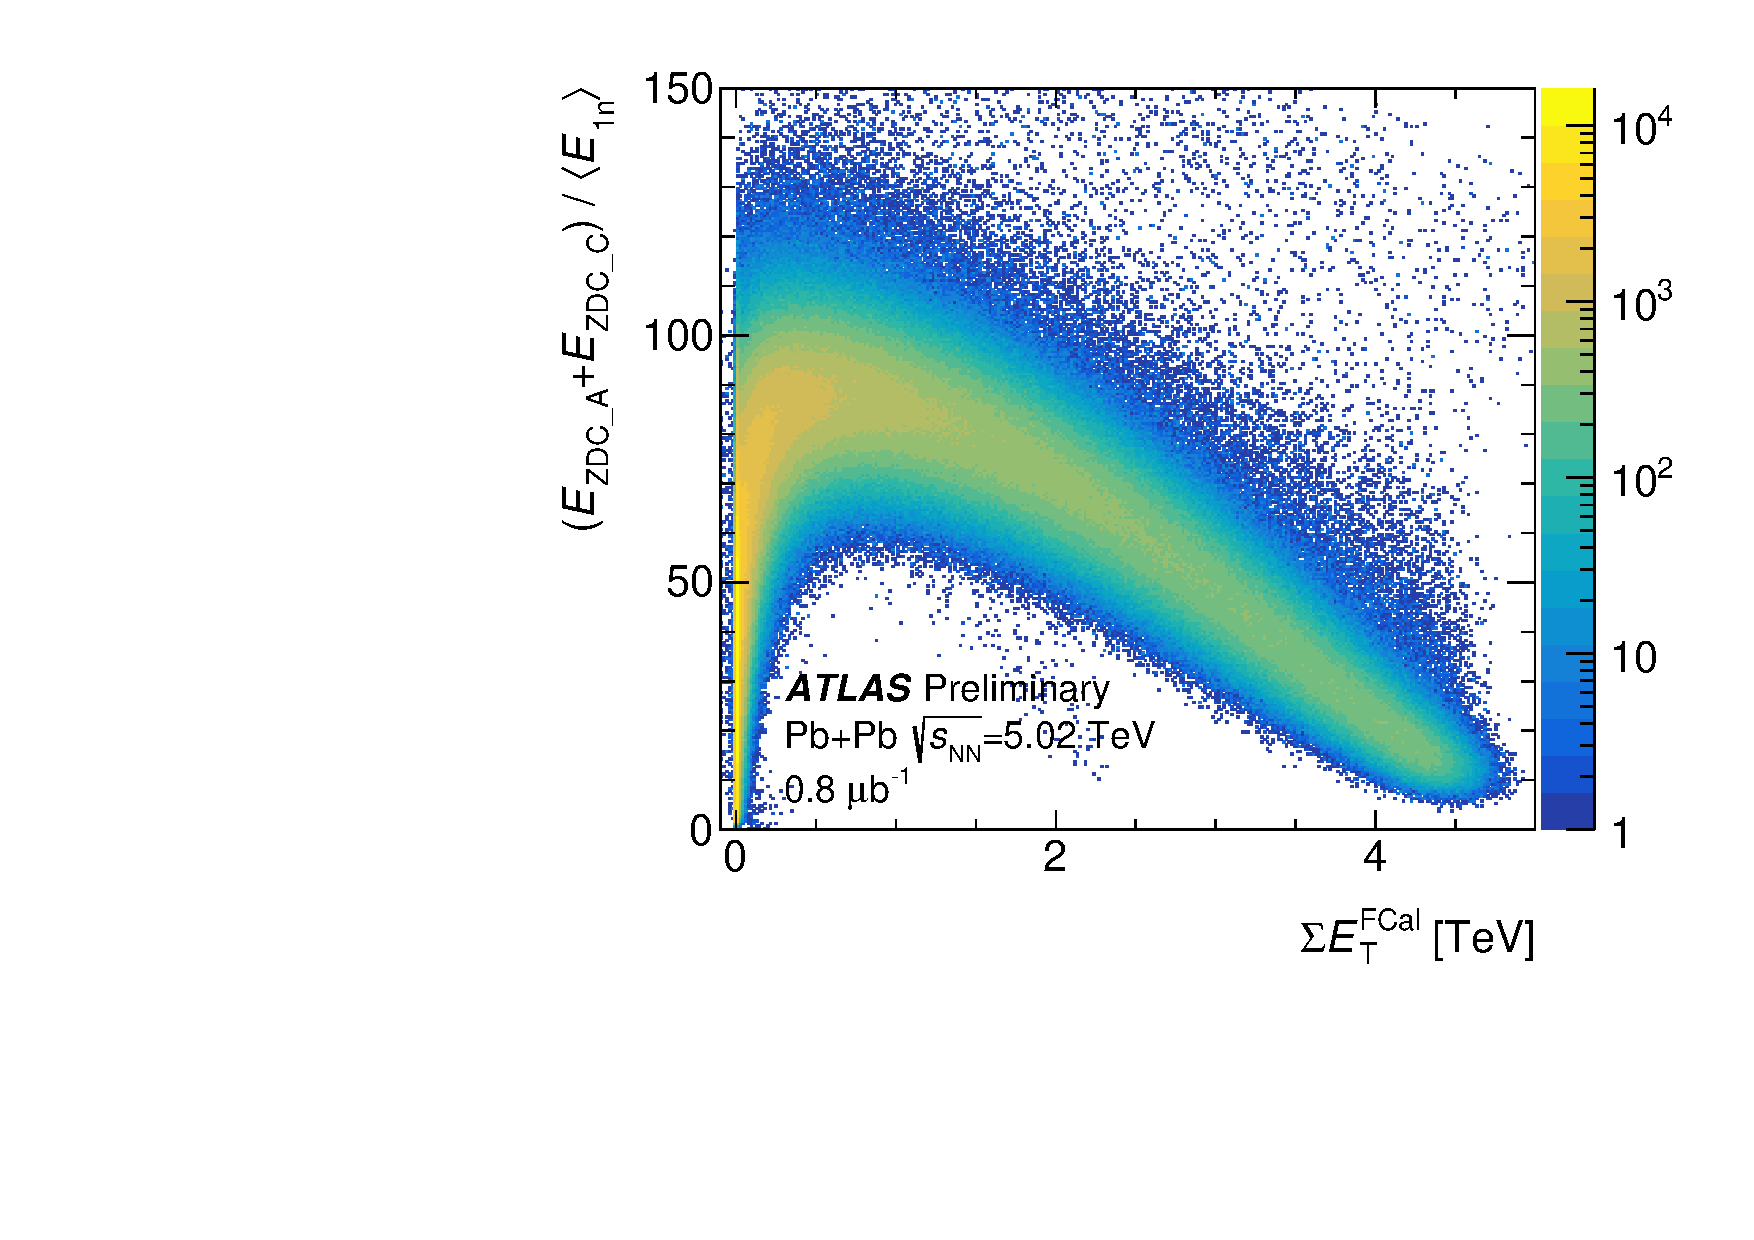
\includegraphics[width=.475\linewidth]{figs/chapter_detector/ATLAS_ZDC_FCal.pdf}
\caption{Left: Energy in the ZDC arm C (negative rapidity), divided by the most probable energy of the single neutron peak. Peaks showing contributions from up to four neutrons emitted in a single event are clearly visible. Right: Correlation of the sum of the energies in the two ZDC arms, normalized to the single neutron energy, v.s. the sum of transverse energies measured in the FCal. For both plots, a reconstructed vertex is also required to be present in each event.}
\label{fig:detector_ATLAS_ZDC_FCal}
\end{figure}



\subsubsection{Minimum-Bias Trigger Scintillators}

Minimum Bias Trigger Scintillators (MBTS)~\cite{Sidoti:2014kra} delivered the primary triggers for selecting events from real LHC collisions with the smallest bias. The MBTS consist of 2 cm thick polystyrene scintillator disks mounted on both sides of the interaction point at a distance of approximately 3.6 m along the beam pipe. Each side has an inner and outer ring in $\eta$ of eight counters in the azimuthal angle $\phi$, as shown in Figure~\ref{fig:detector_ATLAS_MBTS}. The outer counters pseudorapidity acceptance is $2.08 < |\eta| < 2.78$, while the acceptance for inner counters is $2.78 < |\eta| < 3.75$. Wavelength shifting fibers are embedded in grooves at the edges of the counters and are grouped at the center of the module between the two pieces of scintillator. These optical fibers guide the emitted light to PMTs. The MBTS signals, after being shaped and amplified in such a way that the pulse amplitude is proportional to the amount of energy deposited in the counter, are fed into leading edge discriminators and sent as 25 ns pulses to the Central Trigger Processor (CTP). The total charge collected as well as the arrival time of the signal are recorded. An MBTS hit is defined as a signal above the discriminator threshold. At the CTP input, the 32 MBTS signals are stretched to 200 ns and the hit multiplicity is calculated for each side independently. The CTP combines individual signals in L1 trigger items like $\verb|L1_MBTS_1|$, which require at least one hit in the MBTS detectors. The use of MBTS as minimum-bias triggers will be discussed in the data acquisition section.

\begin{figure}[H]
\centering
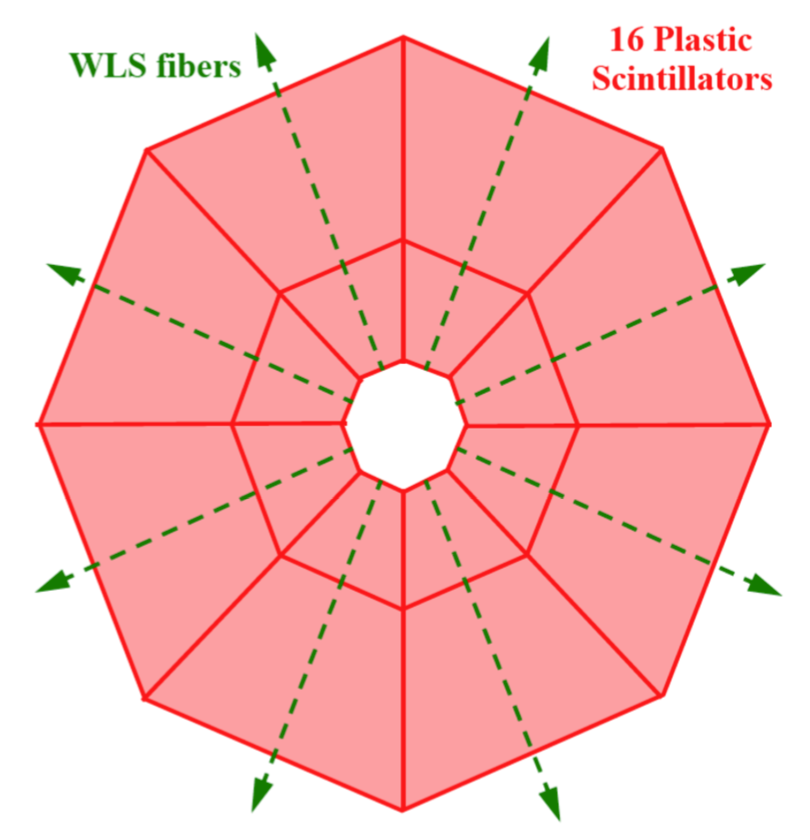
\includegraphics[width=.475\linewidth]{figs/chapter_detector/ATLAS_MBTS.png}
\caption{Layout of one of the two MBTS disks.}
\label{fig:detector_ATLAS_MBTS}
\end{figure}



\subsection{Data acquisition and selection}

The measurements presented in this thesis were gathered from the following data sets:
\begin{itemize}
\item Pb+Pb at $\sqrt{s_\text{NN}}=5.02$ TeV, recorded in 2015;
\item Xe+Xe at $\sqrt{s_\text{NN}}=5.44$ TeV, recorded in 2017;
\item $p$+Pb at $\sqrt{s}=5.02$ TeV, recorded in 2016;
\item $pp$ at $\sqrt{s}=13$ TeV, recorded in 2015 and 2016;
\end{itemize}
In the following sections, we will discuss the trigger, event selection, track selection and tracking efficiency, for each of the datasets above.



\subsubsection{Pb+Pb at $\sqrt{s_\text{NN}}=5.02$ TeV}

The Pb+Pb datasets were obtained from a sample of minimum-bias and ultra-central Pb+Pb collisions at $\sqrt{s_\text{NN}}=5.02$ TeV recorded by ATLAS in 2015 (Run 2). The corresponding integrated luminosity are approximately 470 $\mu b^{-1}$. The measurements were performed using the ATLAS inner detector and forward calorimeters.



\paragraph{Trigger}

The minimum-bias triggers for 5.02 TeV Pb+Pb collisions are:
\begin{itemize}
\item \verb|HLT_mb_sptrk_ion_L1ZDC_A_C_VTE50|
\item \verb|HLT_noalg_mb_L1TE50|
\end{itemize}
where \verb|sptrk| requires at least one reconstructed track at the HLT level, \verb|L1ZDC_A_C| requires at least one hit in both sides of ZDC detector. The major difference between these two triggers is Level-1 (L1) total energy \verb|TE|: \verb|VTE50| requires total energy less than 50 GeV while \verb|TE50| larger than 50 GeV.

To enhance the statistics in ultra-central collisions, Ultra-Central Collision (UCC) triggers are also included:
\begin{itemize}
\item \verb|HLT_hi_th1_ucc_L1TE14000|
\item \verb|HLT_hi_th2_ucc_L1TE14000|
\item \verb|HLT_hi_th3_ucc_L1TE14000|
\end{itemize}
where \verb|L1TE| denotes the minimum L1 total energy cut and \verb|th| corresponds to the various online minimum FCal Calorimeter $\Et$ cut at the High-Level Trigger (HLT) level.

Figure~\ref{fig:detector_ATLAS_trigger_PbPb502} shows the FCal $\Et$ distributions seeded by two major UCC triggers, compared with those seeded by minimum-bias (MinBias) triggers. UCC triggers collected about 20 times more event statistics compared with MinBias trigger in the ultra-central collisions. Furthermore, the turn-on curves of UCC trigger efficiencies are very shape, which means the selection bias caused by these triggers is negligible. The impact from trigger efficiency will be discussed in details in Section~\ref{sec:trigger_selection_bias}.

\begin{figure}[H]
\centering
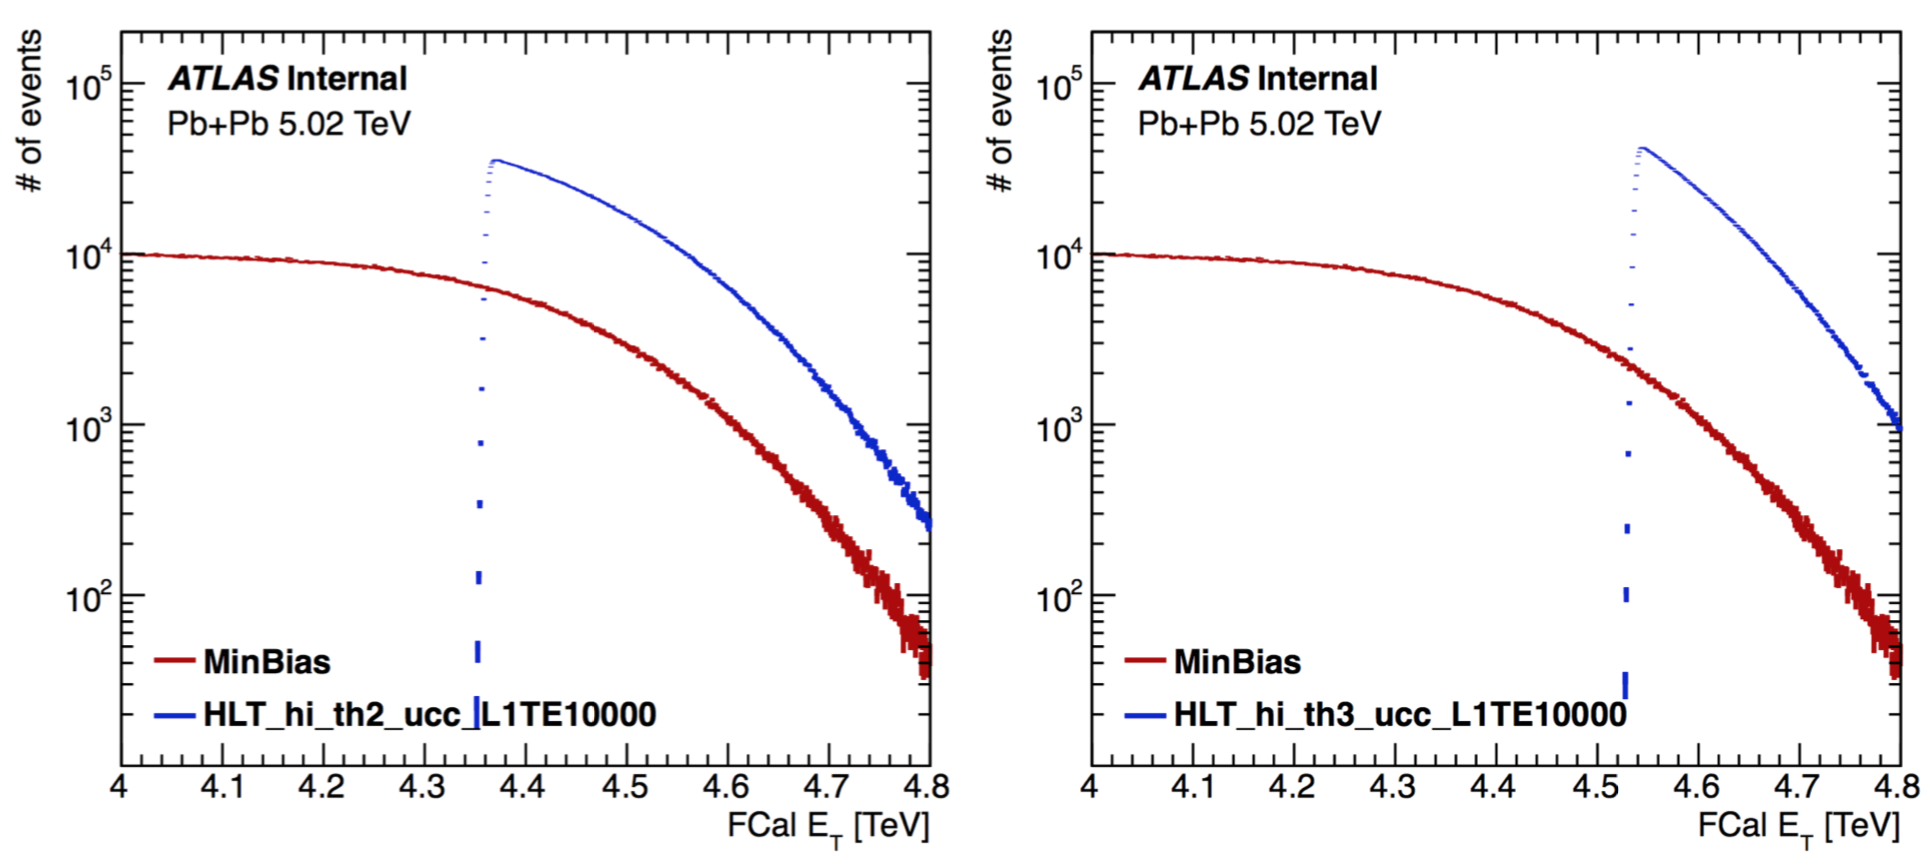
\includegraphics[width=.95\linewidth]{figs/chapter_detector/ATLAS_trigger_PbPb502.png}
\caption{FCal $\Et$ distributions for two major UCC triggers (red points), compared with MinBias trigger (blue points).}
\label{fig:detector_ATLAS_trigger_PbPb502}
\end{figure}



\paragraph{Event selection}
\label{sec:event_selection}

The event selections for 5.02 TeV Pb+Pb events are:
\begin{itemize}
\item Pass Good Run List (GRL);
\item Have a primary reconstructed vertex;
\item Events with detector errors (LAr, Tile, SCT) removed;
\item Vertex position cut: $|z_\text{vtx}|<100$ mm;
\end{itemize}
where the definitions of centrality and pileup events will be discussed below. In this thesis we are cutting the vertex position at 100 mm instead of 150 mm in previous published Pb+Pb analysis. This is because multiplicity distribution along $\eta$ changes with $z_\text{vtx}$ position, which might have a minor impact on forward-backward analysis and subevent cumulant analysis, since those analyses are highly $\eta-$dependent. In order to avoid introducing large multiplicity fluctuations in the forward $\eta$ region, we further constrain the vertex position to 100 mm, and we will not loose much statistics with this tighter cut.

In the 2015 Pb+Pb run, the luminosity conditions provided by the LHC result in an average probability of $0.1\%$ that an event contains two or more Pb+Pb collisions (pileup). The pileup events are suppressed by only using the tracks from primary vertex. The remaining pileup events are further suppressed on the correlation between energies deposited in FCal and ZDC. This signal in the ZDC is calibrated to the number of detected neutrons $N_n$ based on the location of the peak corresponding to a single neutron. Figure~\ref{fig:detector_ATLAS_pileup_PbPb502} shows the procedure of pileup rejection and its performance. The left panel shows the correlation between number of neutrons in the ZDC and total transverse energy $\Et$ in the FCal. The ``banana''-shaped main band covers the events with a single vertex. While in a pileup event, both the number of neutrons and FCal $\Et$ are larger than those from a single event, and this is illustrated by the events in the ``grass'' region above the main band. To clean up the pileup, one way is by applying a linear cut on the correlation map, indicated by the black straight line, and another approach is cutting off $0.1\%$ of the events in the tails of $N_\text{neutrons}$ distribution in each FCal $E_\text{T}$ slice, indicated by the red curve. In this analysis, we will use the $0.1\%$ cut as the default cut. The right panel shows the performance of the two pileup rejection methods just mentioned. The Y-axis represents the fraction of rejected pileup events out of all the pileup events. The rejection rate is low at low FCal $\Et$, this is because the band for pileup events mostly overlaps with the main band for single events. However, since the fraction of pileup events is very low in peripheral collisions, the low rejection rate has no impact on the results. On the other hand, the rejection rate reaches $100\%$ in UCC, where the fraction of pileup event is high, meaning that almost all the pileup events are rejected using this $0.1\%$ pileup cut. The systematics relating to the pileup cut will be discussed in Section~\ref{sec:pileup_rejection}.

\begin{figure}[H]
\centering
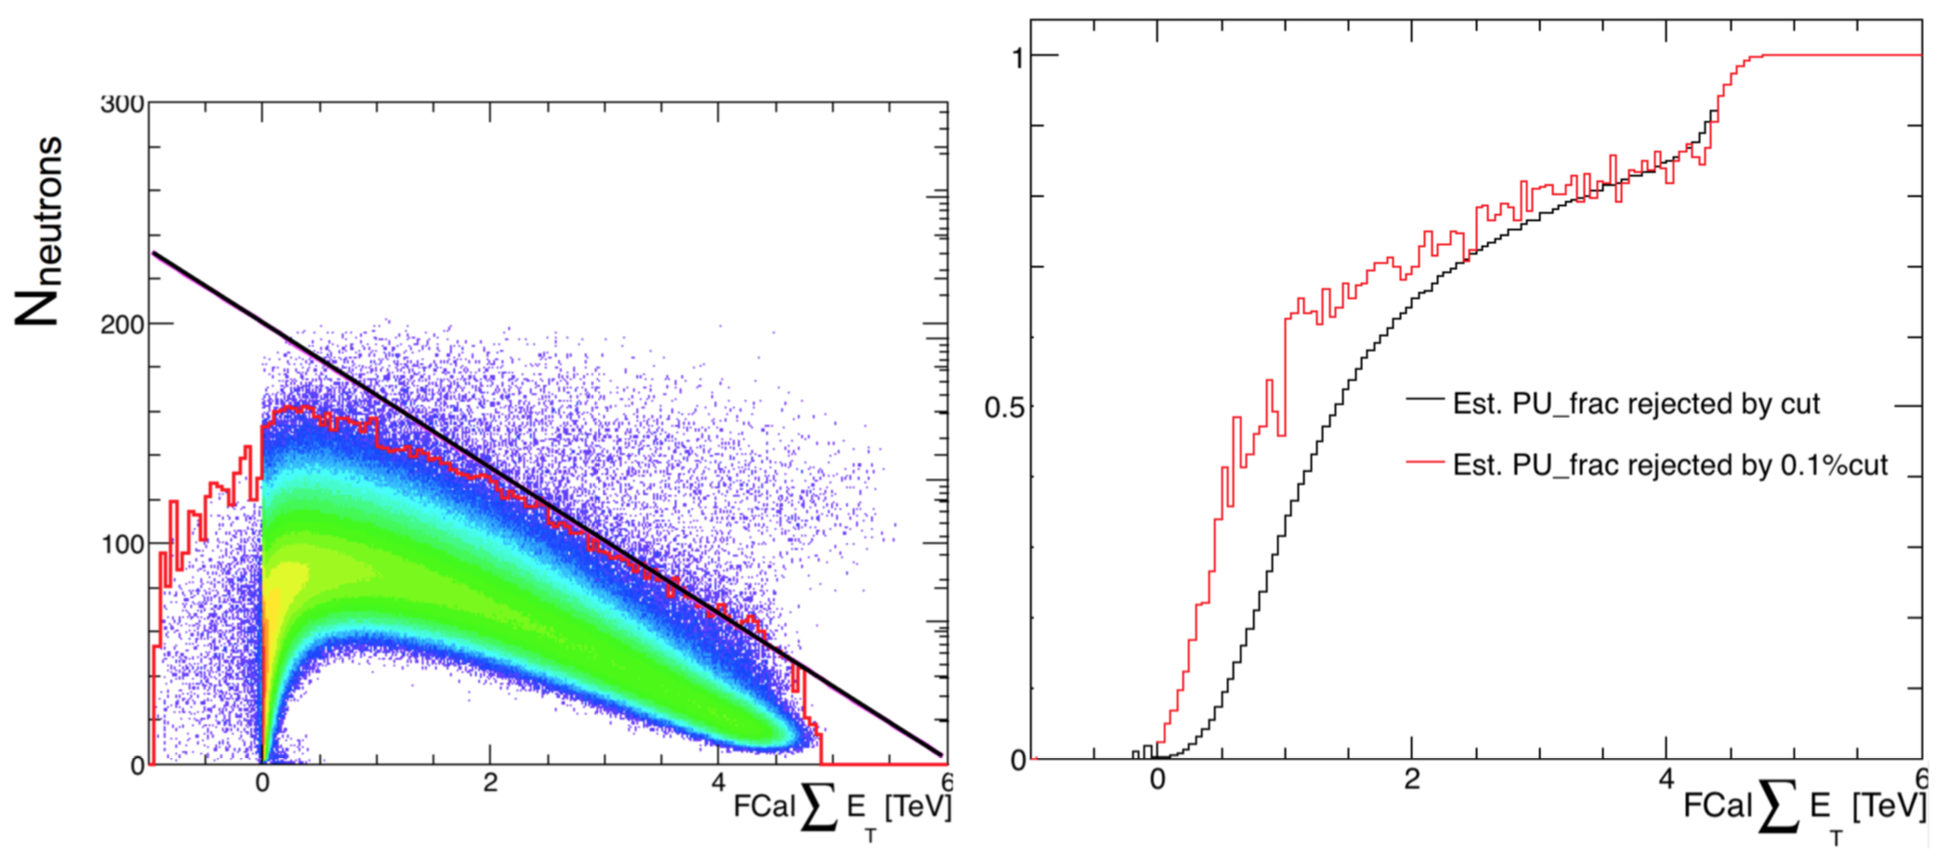
\includegraphics[width=.95\linewidth]{figs/chapter_detector/ATLAS_pileup_PbPb502.png}
\caption{Left: the correlation between calibrated number of neutrons in the ZDC and FCal $\Et$. Right: the fraction of rejected pileup events in all pileup events. Two rejection criteria are shown: a linear cut and $0.1\%$ cut.}
\label{fig:detector_ATLAS_pileup_PbPb502}
\end{figure}



\paragraph{Centrality determination}
\label{sec:centrality_determination}

The heavy-ion collision geometry is defined by its impact parameter $b$. As the actual event-by-event impact parameter is not accessible experimentally, the centrality classification is based on the transverse energy measured in the FCal, $\Et^\text{FCal}$, which exhibits a strong monotonic correlation with $b$. A model based on the Monte Carlo (MC) Glauber approach~\cite{Miller:2007ri} is used to obtain the mapping from the observed $\Et^\text{FCal}$ to the primary properties, such as the number of binary nucleon-nucleon interactions, $N_\text{coll}$, or the number of nucleons participating in the nuclear collision, $N_\text{part}$, for each centrality interval. The Glauber model also provides a correspondence between the $\Et^\text{FCal}$ distribution and the sampling fraction of the total inelastic Pb+Pb cross-section, allowing the setting of the centrality percentiles. For this analysis a selection of the $80\%$ most central collisions (i.e. centrality 0-80$\%$) is used to avoid any diffractive, photonuclear, and other inelastic process that contribute significantly to very peripheral collisions. Figure~\ref{fig:detector_ATLAS_centrality_PbPb276} shows the distribution of $\Et^\text{FCal}$ in the 2.76 TeV Pb+Pb data, and thresholds for the selection of several centrality intervals. Uncertainties of centrality determination are shown in Section~\ref{sec:centrality_definition}.

\begin{figure}[H]
\centering
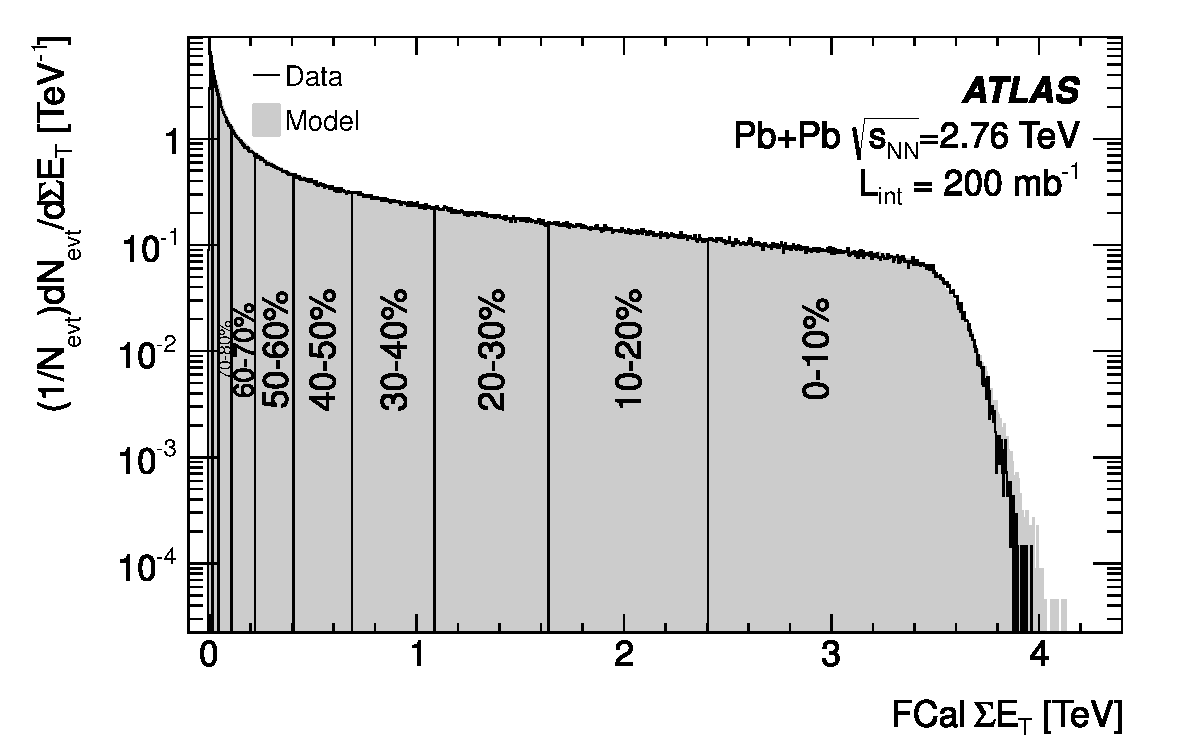
\includegraphics[width=.6\linewidth]{figs/chapter_detector/ATLAS_centrality_PbPb276.pdf}
\caption{Measured $\Et^\text{FCal}$ distribution divided into $10\%$ centrality intervals (black). This figure is taken from Ref.~\cite{ATLAS:2011ah}}
\label{fig:detector_ATLAS_centrality_PbPb276}
\end{figure}



\paragraph{Track selection, efficiency and fake rate}
\label{sec:track_selection_efficiency_and_fake_rate}

The default track selection for the Pb+Pb analysis is HILoose, which is defined as:
\begin{itemize}
\item number of pixel hits $> 0$;
\item number of SCT hits + dead sensors $\geq 6$;
\item if IBL hit is expected: at least 1 IBL hit required;
\item if no IBL hit is expected: a Layer-0 hit if expected;
\item $|d_0| \leq 1.5$ mm;
\item $|z_0 - z_\text{vtx}|\text{sin}\theta \leq 1.5$ mm;
\end{itemize}
where $d_0$ is the minimum transverse distance between a track and its associated vertex, and $z_0$ is the minimum longitudinal distance between a track and vertex. In Section~\ref{sec:track_selection}, a tighter cut, HITight, is applied to check the stability of tracking reconstruction.

To estimate the tracking efficiency and fake rate, HIJING MC samples with similar detector conditions are used. For the reconstructed tracks, the primary tracks, $N_\text{ch}^\text{primary}$, are defined as:
\begin{itemize}
\item pass the HILoose track quality selection;
\item truth match probability $>0.5$;
\item associated truth particle is a primary particle;
\end{itemize}
where truth match probability measures the probability of a reconstructed track matched to its truth track. The primary particle is defined at the truth level:
\begin{itemize}
\item status = 1, charge $!=$ 0;
\item 0 $<$ Barcode $<$ 2E5;
\item strange baryons are excluded;
\end{itemize}

The tracking efficiency $\epsilon$ can then be defined as:
\begin{equation}
\epsilon(\pT, \eta, \text{centrality}) \equiv \frac{N_\text{ch}^\text{primary}}{N_\text{ch}^\text{truth}},
\end{equation}
where $N_\text{ch}^\text{truth}$ denotes the number of primary particles at the truth level, all of which passed the HILoose track quality selection.

The tracking efficiency map is evaluated as a function of $\pT$, $\eta$ and centrality, and the results are shown in Figure~\ref{fig:detector_ATLAS_track_eff_PbPb502}, for different $\pT$ ranges and centralities. $\epsilon(\eta)$ is highest in mid-rapidity $-1<\eta<1$, and decrease by $20\%$ in forward-rapidity. As collision moves to peripheral, the efficiency increases. The tracking efficiency slightly increases towards higher $\pT$. Efficiency from HILoose is higher than HITight as expected.

\begin{figure}[H]
\centering
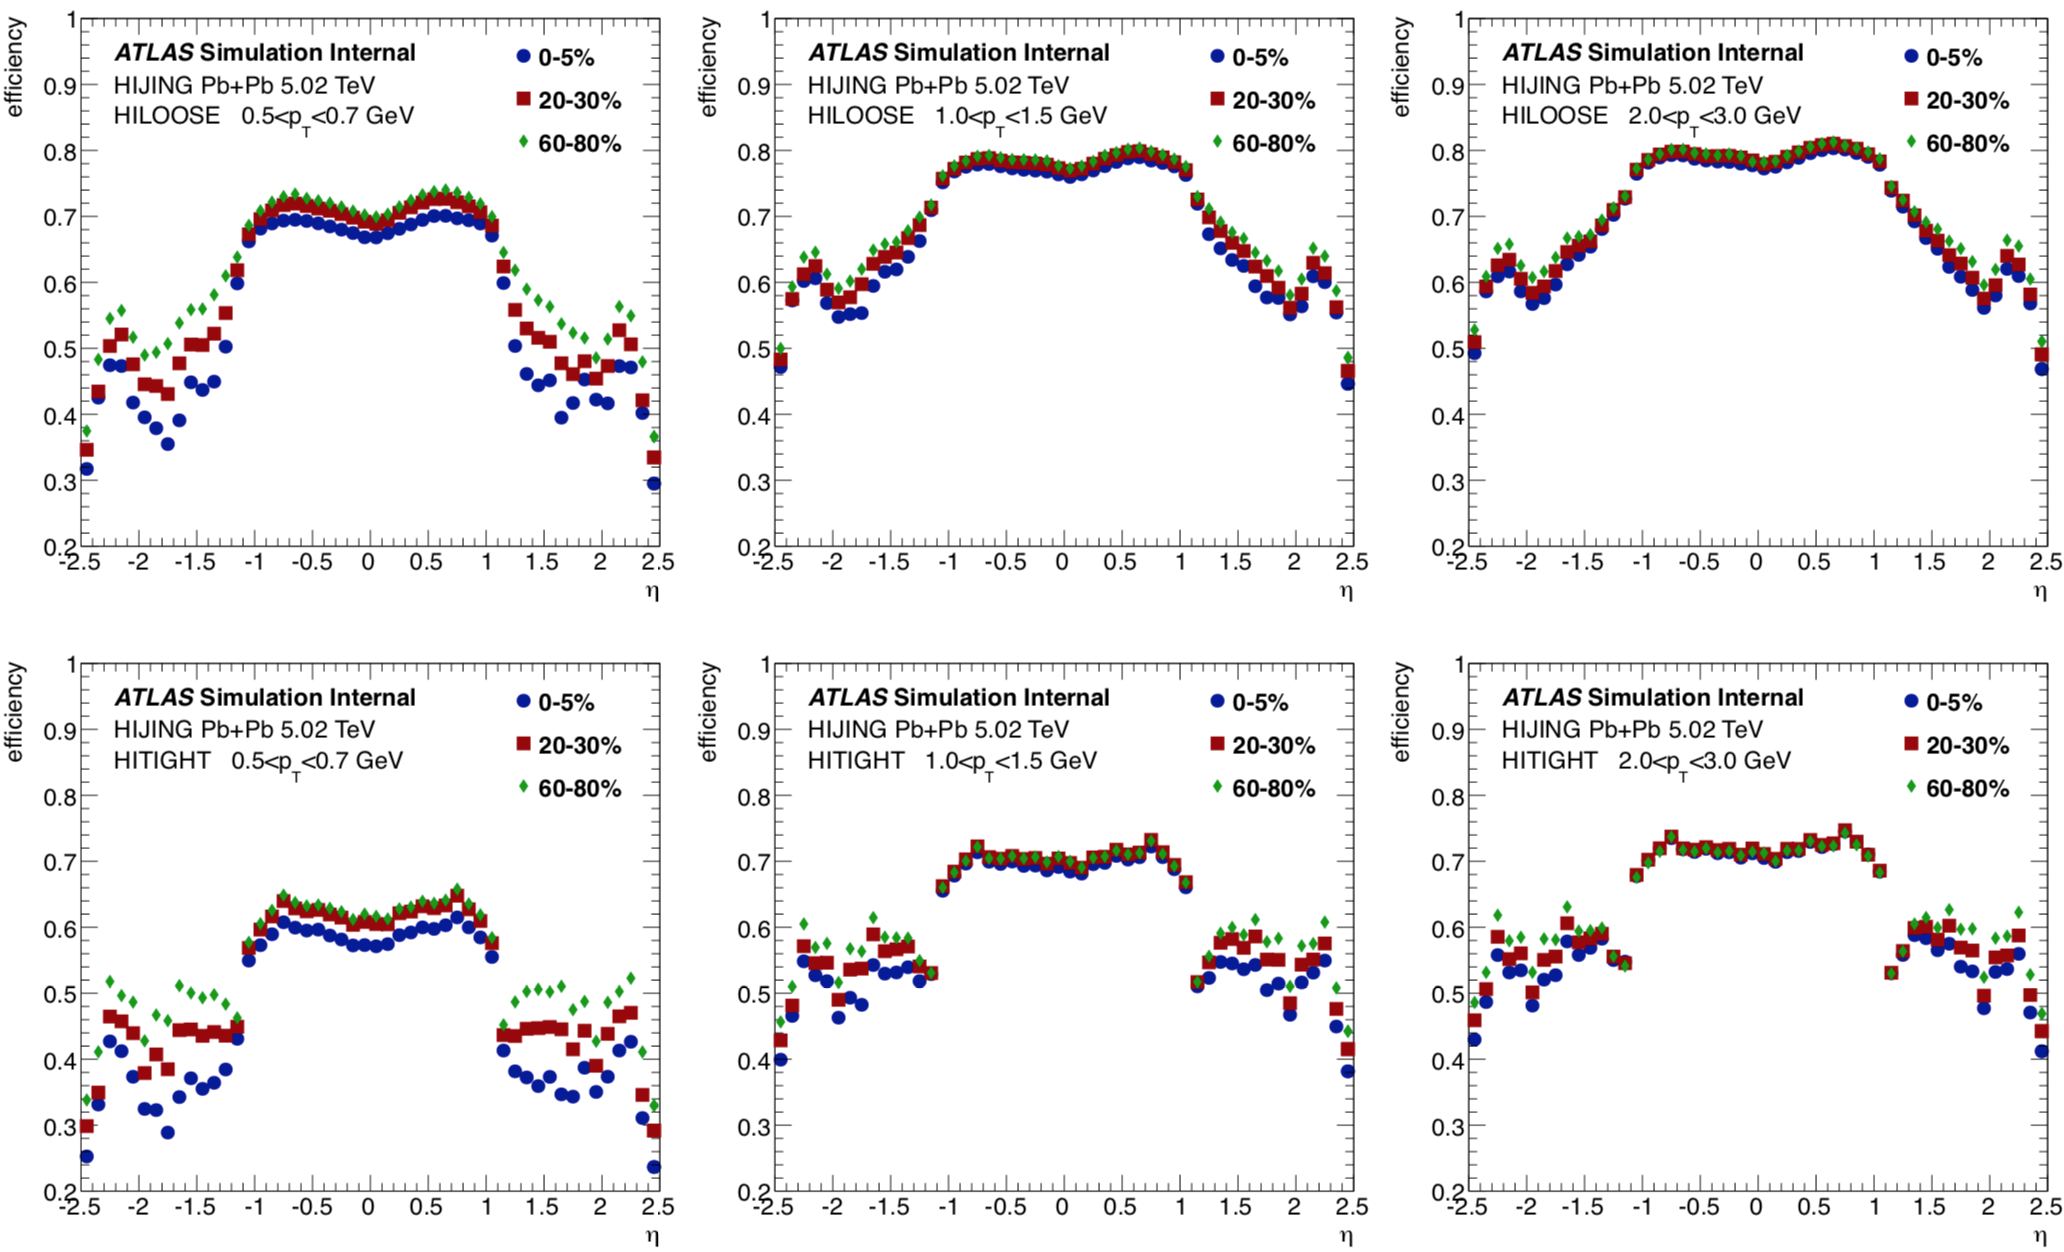
\includegraphics[width=.95\linewidth]{figs/chapter_detector/ATLAS_track_eff_PbPb502.png}
\caption{5.02 TeV Pb+Pb tracking efficiency $\epsilon(\eta)$, for different $\pT$ ranges and centralities. Top row is for HILoose and bottom row is for HITight.}
\label{fig:detector_ATLAS_track_eff_PbPb502}
\end{figure}

The fake track is defined as:
\begin{itemize}
\item pass the HILoose track quality selection;
\item fulfill one of the following:
\begin{itemize}
\item truth match probability $<0.5$;
\item not associate with truth particles;
\item Barcode = 0 of associated truth particle;
\end{itemize}
\end{itemize}

The faction of fake tracks (fake rate) $f$ is defined as:
\begin{equation}
f(\pT, \eta, \text{centrality}) \equiv \frac{N_\text{ch}^\text{fake}}{N_\text{ch}^\text{primary} + N_\text{ch}^\text{fake}},
\end{equation}
where $N_\text{ch}^\text{fake}$ denotes the number of fake tracks.

One of the focuses of our studies is on UCC collisions, where fake rate is significantly higher than MB events. The fake rates map is evaluated as a function of $\pT$, $\eta$ and centrality, and the results are shown in Figure~\ref{fig:detector_ATLAS_track_fake_PbPb502}. $f(\eta)$ is lowest in mid-rapidity $-1<\eta<1$, and increases by more than two times in forward-rapidity. As collision moves to peripheral, the fake rate significantly deceases. The fake rate decreases significantly towards higher $\pT$.

\begin{figure}[H]
\centering
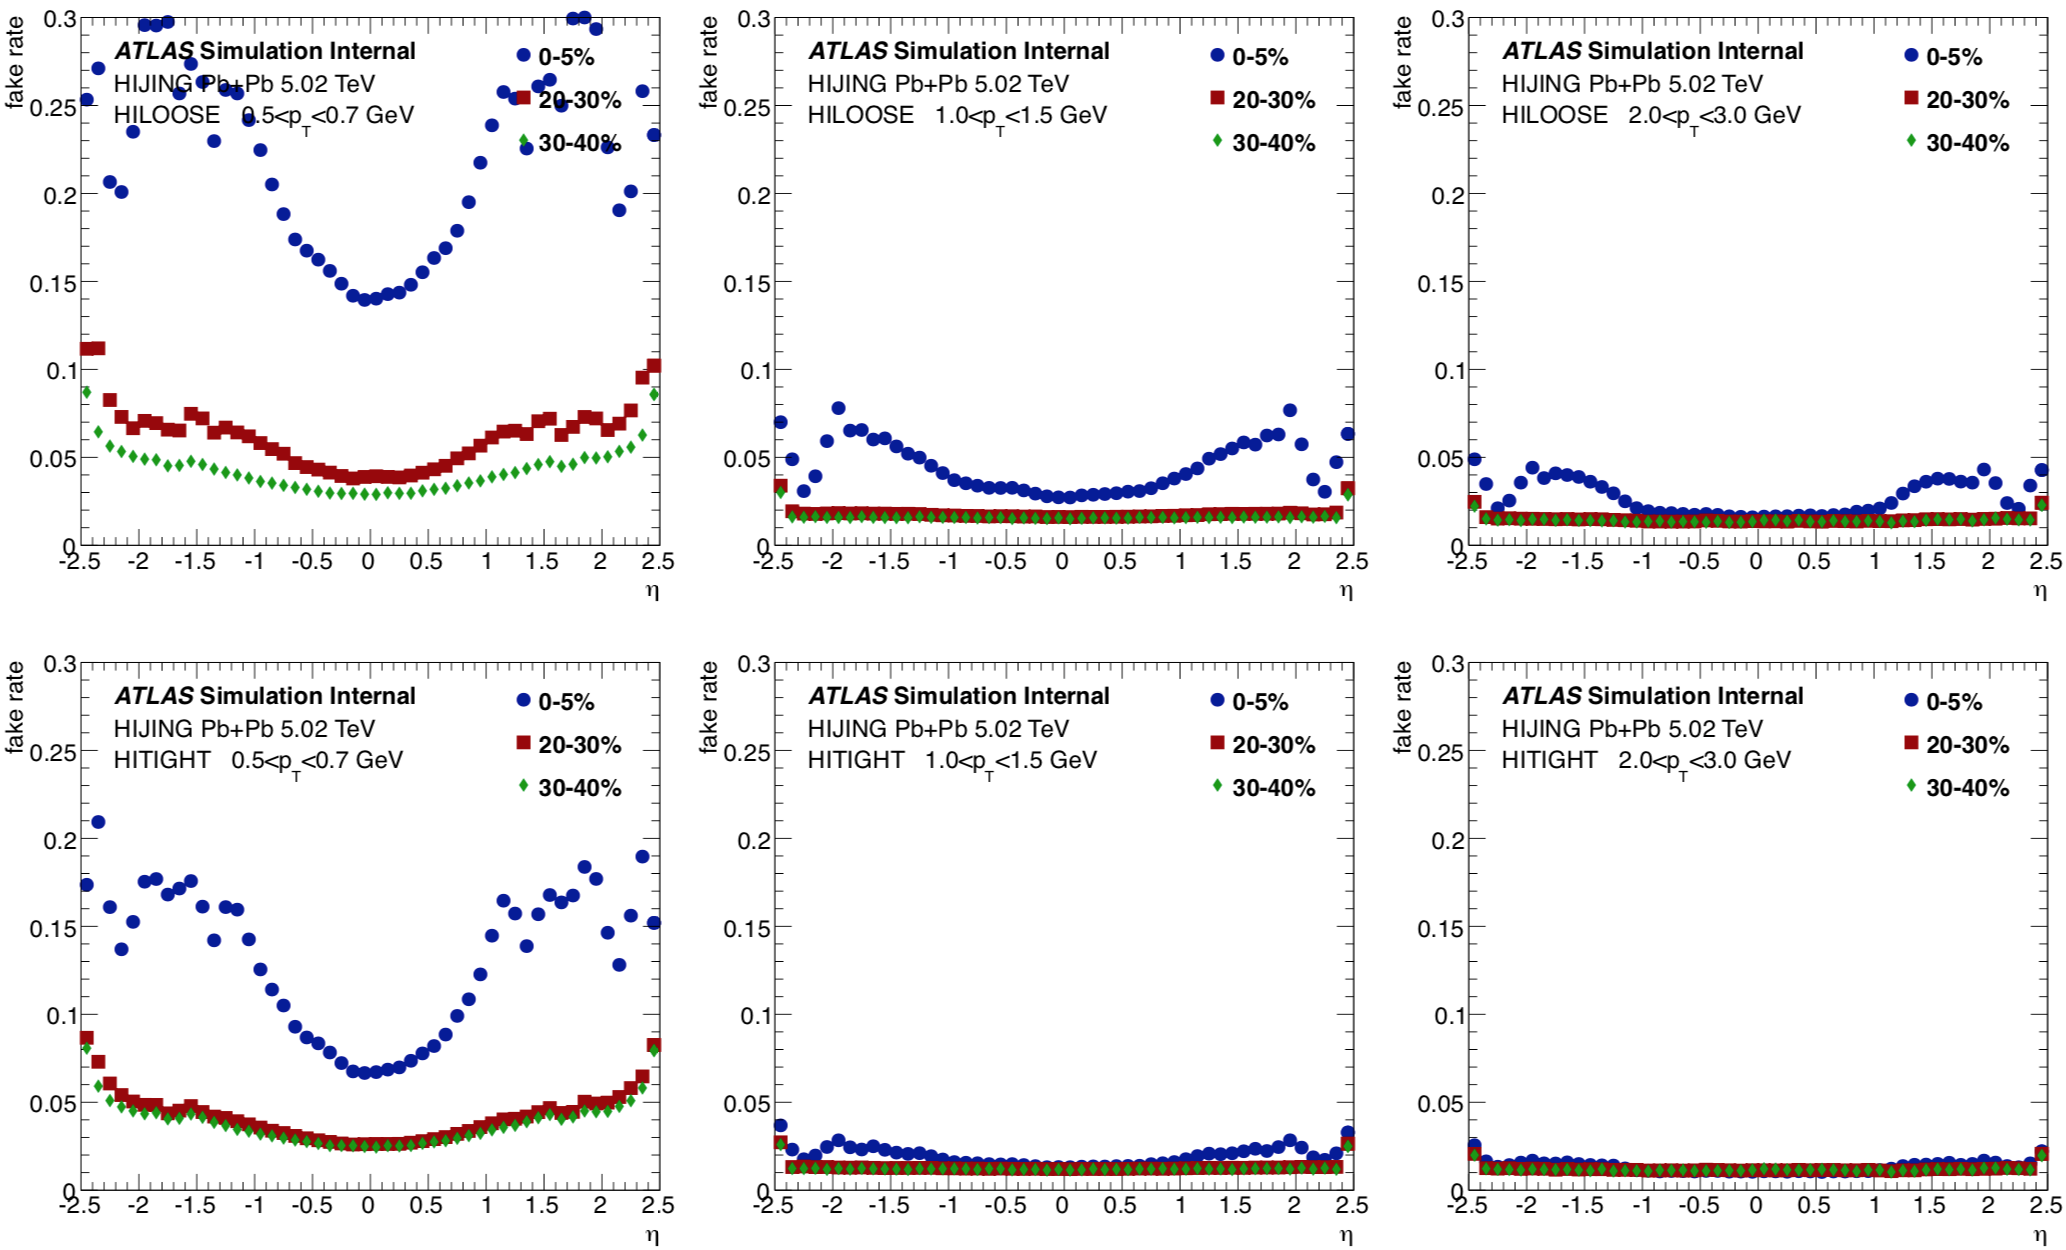
\includegraphics[width=.95\linewidth]{figs/chapter_detector/ATLAS_track_fake_PbPb502.png}
\caption{5.02 TeV Pb+Pb tracking fake rates $f(\eta)$, for different $\pT$ ranges and centralities. Top row is for HILoose and bottom row is for HITight.}
\label{fig:detector_ATLAS_track_fake_PbPb502}
\end{figure}

To compensate the contribution from fake tracks, the efficiency $\epsilon$ can be corrected by defining $\epsilon'$:
\begin{equation}
\epsilon'(\pT, \eta, \text{centrality}) \equiv \frac{N_\text{ch}^\text{primary} + N_\text{ch}^\text{fake}}{N_\text{ch}^\text{truth}} = \frac{\epsilon}{1+f}
\end{equation}
where an additional correction of fake rates $1-f$ is added to the tracking efficiency $\epsilon$. In the analysis, we varied the tracking efficiency within its uncertainties to test the stability of the measurements, and the results are shown in Section~\ref{sec:tracking_efficiency}.



\subsubsection{Xe+Xe at $\sqrt{s_\text{NN}}=5.44$ TeV}

The Xe+Xe analysis uses data from the 2017 LHC Xe+Xe run at $\sqrt{s_\text{NN}}=5.44$ TeV. The data were recorded during a single 8 hour fill in October 2017. The data were recorded into several streams. This analysis uses data from the MinBias stream only.



\paragraph{Trigger}

The MinBias events were recorded by the following two triggers:
\begin{itemize}
\item \verb|HLT_mb_sptrk_L1MBTS_1_VTE4|: At level-1, this trigger requires less than 4 GeV transverse energy in the calorimeter together with a signal in one of the MBTS detectors. At the high level trigger, this requires one reconstructed track. This trigger is meant to select peripheral events;
\item \verb|HLT_noalg_mb_L1TE4|: This trigger simply requires that the L1 transverse energy to be greater than 4 GeV;
\end{itemize}

During the data collection, none of the events passed \verb|L1VTE4| without prescale, and the prescale value varies between 3.3 and 8.0. On the other hand, all the events passed \verb|L1TE4| trigger without prescaling. To properly include the events that passed trigger \verb|L1VTE4|, an event weight $w_\text{trig}$ has been applied to the measured observable. As a summary, the FCal $\Et$ distributions with different trigger selections are shown in Figure~\ref{fig:detector_ATLAS_trigger_XeXe544}. Without $w_\text{trig}$ weight, the combined distribution shows a depletion for FCal $\Et<40$ GeV, which disappears after $w_\text{trig}$ is applied. Since the prescale for \verb|L1TE4| is one, with and without $w_\text{trig}$ weighting have no effects on the $\Et$ distribution.

\begin{figure}[H]
\centering
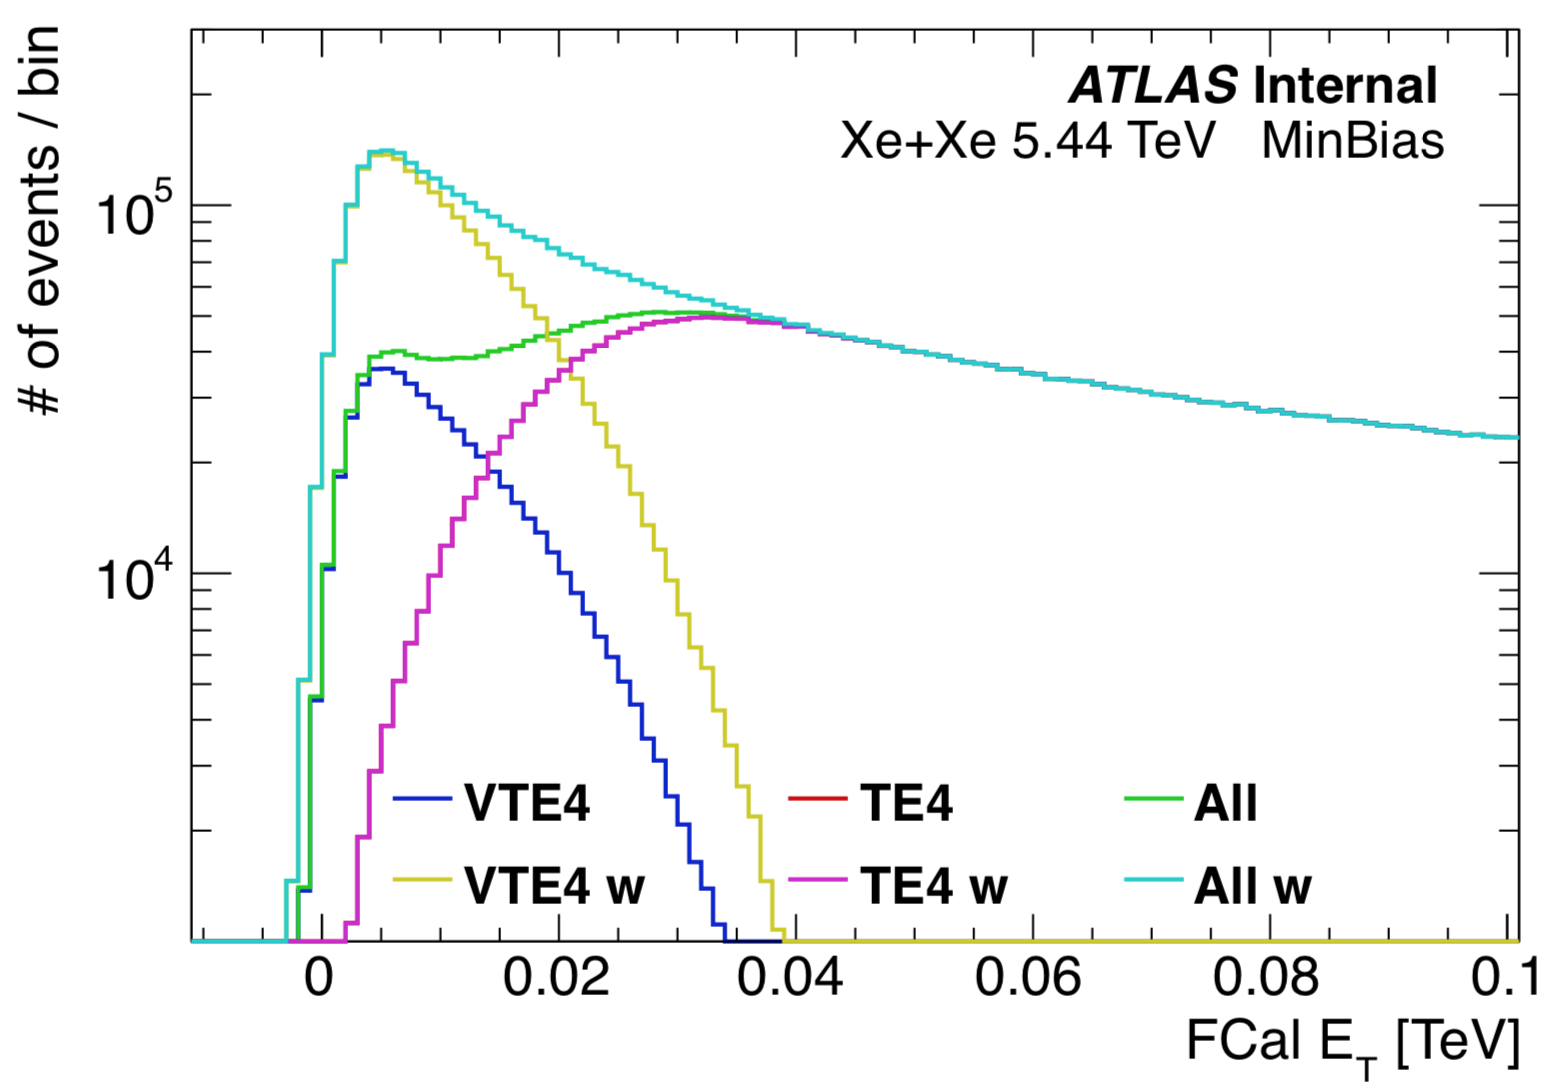
\includegraphics[width=.6\linewidth]{figs/chapter_detector/ATLAS_trigger_XeXe544.png}
\caption{FCal $\Et$ distributions with different trigger selections. ``All'' combines the events passing L1VTE4 and L1TE4. ``w'' meas the distributions are $w_\text{trig}$ weighted.}
\label{fig:detector_ATLAS_trigger_XeXe544}
\end{figure}



\paragraph{Event selection}

The basic event selection of Xe+Xe is exactly the same as Pb+Pb, as discussed in Section~\ref{sec:event_selection}.

During the Xe+Xe run the peak $\mu$ is about 0.00019 and the peak luminosity is 0.000211e30 $\text{cm}^{-2}\text{s}^{-1}$, thus the expected fraction of pileup events is not high. In this analysis pileup rejection is done utilizing the tight correlation between the FCal $\Et$ and the number of reconstructed tracks associated with the primary vertex, as shown in Figure~\ref{fig:detector_ATLAS_FCal_Nch_XeXe544}. The tightly correlated band seen along the diagonal is the correlation from events with a single vertex. Pileup events typically have a much larger FCal $\Et$ at the same value of $\Nchrec$, since $\Nchrec$ denotes the number of tracks associated with the primary vertex and is not affected by pileup. While the FCal $\Et$ is larger due to the additional tracks from the pileup vertex. The pileup events can be rejected by removing events with large FCal $\Et$, at a given $\Nchrec$ such that the event lies outside the tight correlation band between the $\Nchrec$ and the FCal $\Et$. This is shown in Figure~\ref{fig:detector_ATLAS_FCal_Nch_XeXe544} by the red lines. The fraction of events rejected by this cut is approximately $0.1\%$. This cut does not reject pileup events where the FCal $\Et$ is only modified slightly such that they fall within the diagonal band. However, including such events does not affect the analysis, as they only have slightly wrong values of FCal $\Et$ assigned to them, and therefore have only a small error in the assigned centrality.

\begin{figure}[H]
\centering
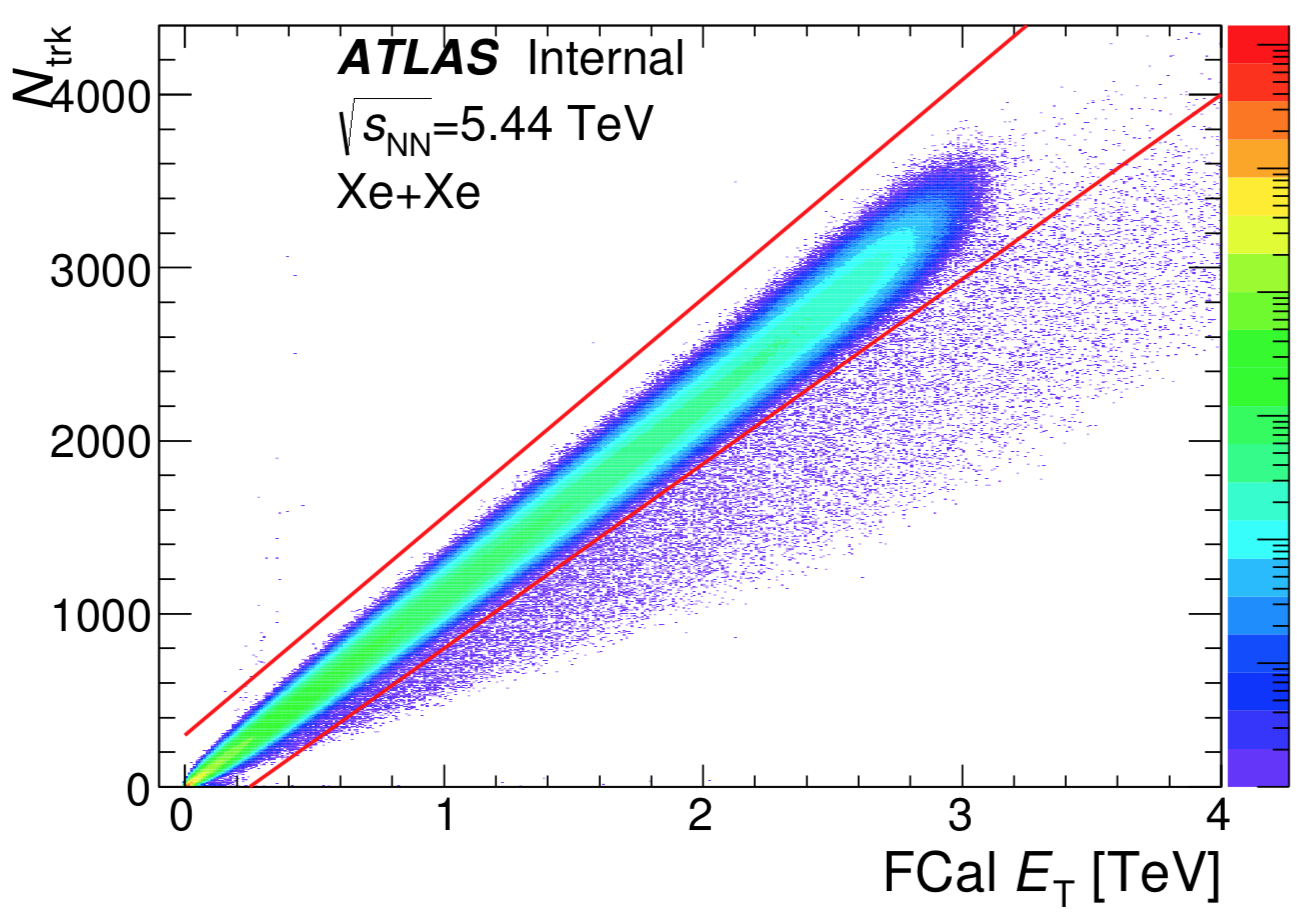
\includegraphics[width=.6\linewidth]{figs/chapter_detector/ATLAS_FCal_Nch_XeXe544.png}
\caption{The correlation between FCal $\Et$ and the number of reconstructed tracks (without any restriction on $\pT$ or quality). The red lines show fiducial cuts to reject pileup and other bad events.}
\label{fig:detector_ATLAS_FCal_Nch_XeXe544}
\end{figure}



\paragraph{Centrality determination}

The MinBias events are binned into centrality percentiles based on the FCal $\Et$. The left panel of Figure~\ref{fig:detector_ATLAS_centrality_XeXe544} shows the FCal $\Et$ distribution for the events used in this analysis, together with the defined centrality classes. The right panel shows the centrality distributions for the MinBias events.

\begin{figure}[H]
\centering
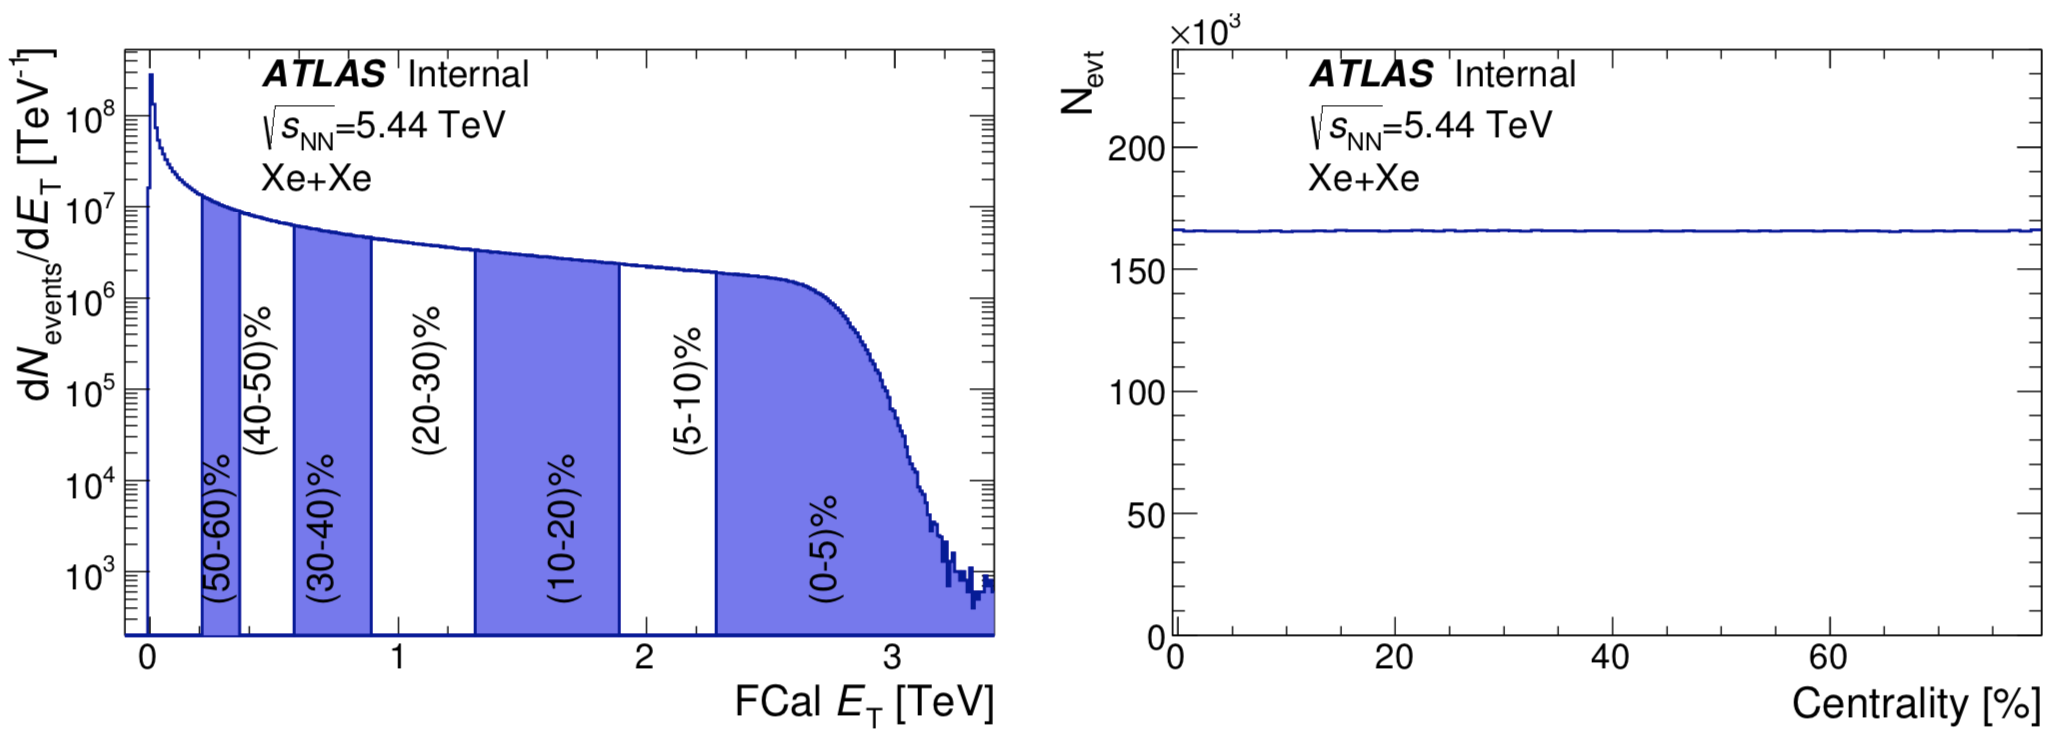
\includegraphics[width=.95\linewidth]{figs/chapter_detector/ATLAS_centrality_XeXe544.png}
\caption{Left: The FCal $\Et$ distribution in MinBias events together with the binning used to define some of the centrality classes. Right: The centrality distribution for MinBias events over the $0-80\%$ centrality interval.}
\label{fig:detector_ATLAS_centrality_XeXe544}
\end{figure}

It is interesting to note that the FCal $\Et$ distribution for the Xe+Xe events has a very similar shape to that seen in previously shown Pb+Pb events. This is shown in Figure~\ref{fig:detector_ATLAS_centrality_XePb}, where after scaling the Pb+Pb FCal $\Et$ distribution by an empirical factor of 0.65, it nearly coincides with the Xe+Xe distribution. It is also interesting to note that the number of nucleons in Xe+Xe is approximated 0.62 (129/208) of the number of nucleons in Pb. Nonetheless, an independent centrality cuts were established for Xe+Xe.

\begin{figure}[H]
\centering
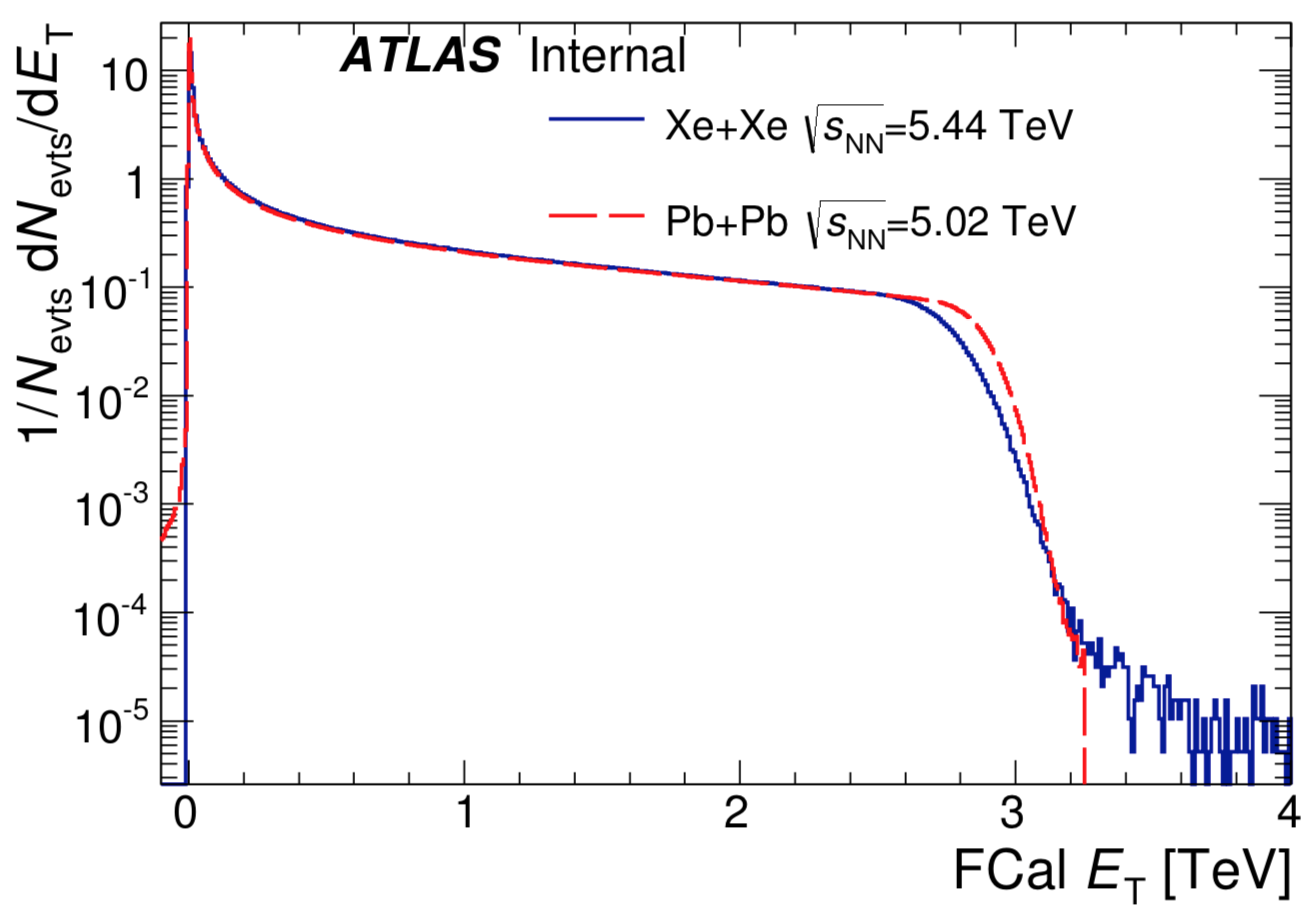
\includegraphics[width=.6\linewidth]{figs/chapter_detector/ATLAS_centrality_XePb.png}
\caption{Comparison between the FCal $\Et$ distribution in Pb+Pb events at $\sqrt{s_\text{NN}}=5.02$ TeV, and the Xe+Xe events at $\sqrt{s_\text{NN}}=5.44$ TeV. The $\Et$ distribution for Pb+Pb events is scaled by an empirical factor of 0.65.}
\label{fig:detector_ATLAS_centrality_XePb}
\end{figure}



\paragraph{Track selection, efficiency and fake rate}

The track selection for Xe+Xe is exactly same as Pb+Pb discussed in previous section. Performance of tracking cuts was established in the MC sample of simulated one million HIJING events. The tracking performance depends on the overall event activity (especially the fake rate) therefore it is obtained from the MC events of similar multiplicities to data. For that, for each centrality bin in data the track multiplicity was obtained. Then efficiency and fake rates were obtained from MC for matching multiplicities. The procedure is identical to the one used for Pb+Pb data described in previous section. Figure~\ref{fig:detector_ATLAS_track_eff_XeXe544} and Figure~\ref{fig:detector_ATLAS_track_fake_XeXe544} show efficiency and fake rates, for different $\pT$, $\eta$ and centrality ranges.

\begin{figure}[H]
\centering
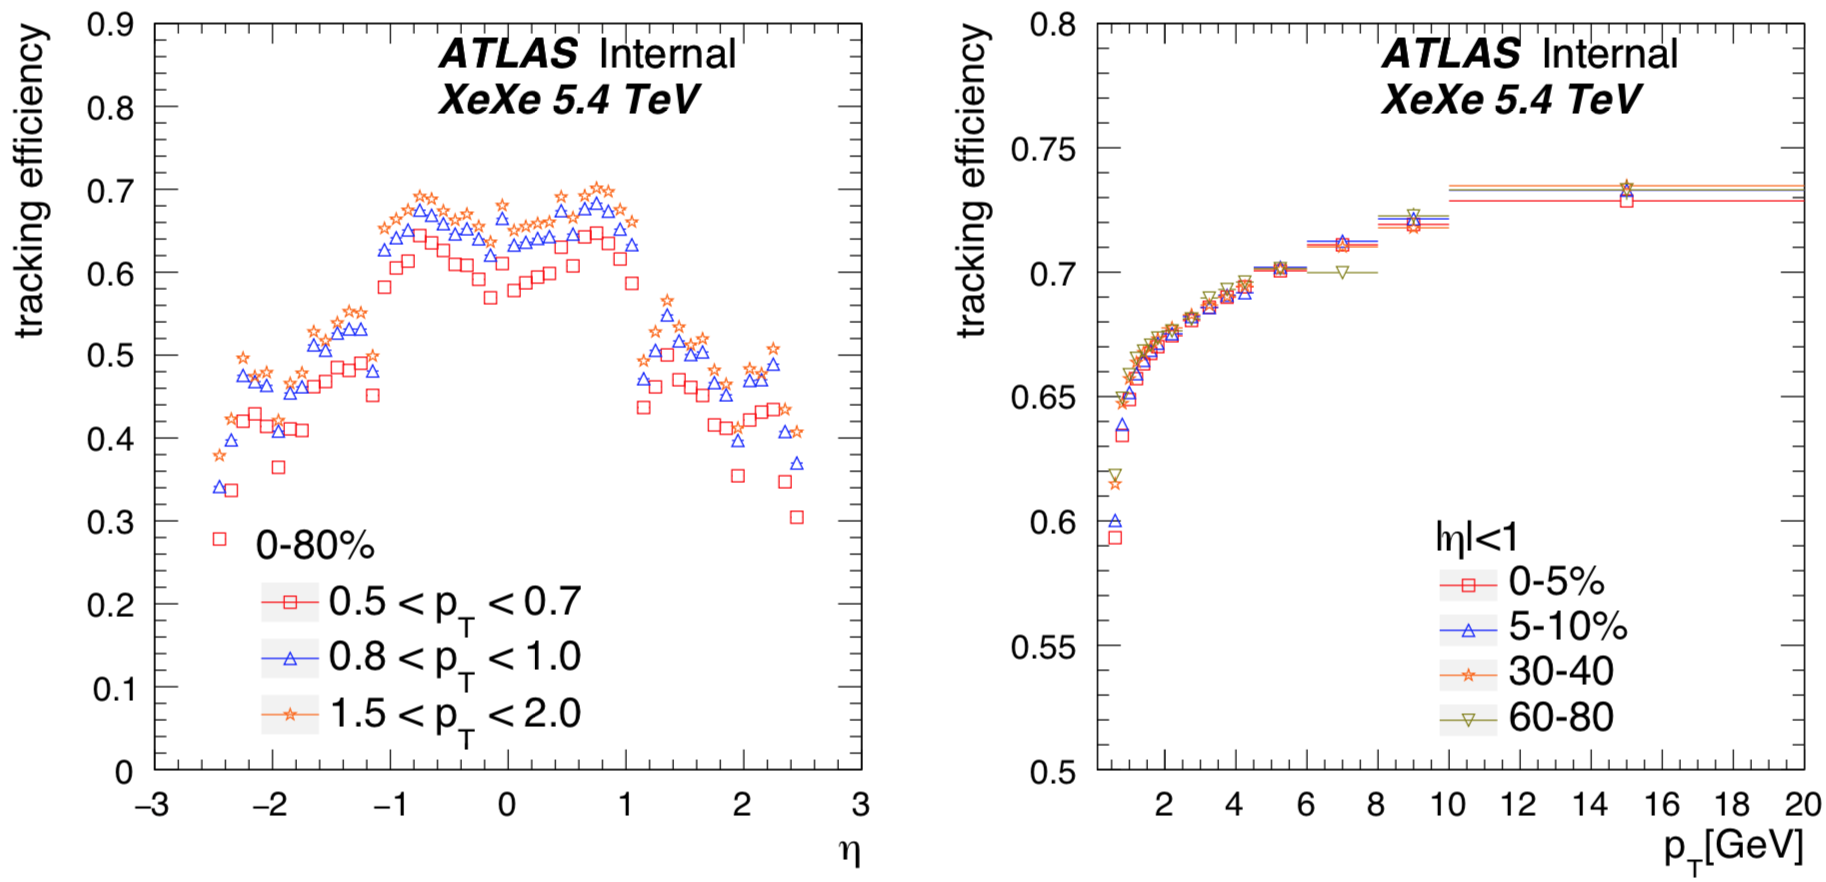
\includegraphics[width=.95\linewidth]{figs/chapter_detector/ATLAS_track_eff_XeXe544.png}
\caption{Tracking efficiency as a function of $\eta$ (left) and $\pT$ (right) for selected centrality and $\pT$ ranges.}
\label{fig:detector_ATLAS_track_eff_XeXe544}
\end{figure}

\begin{figure}[H]
\centering
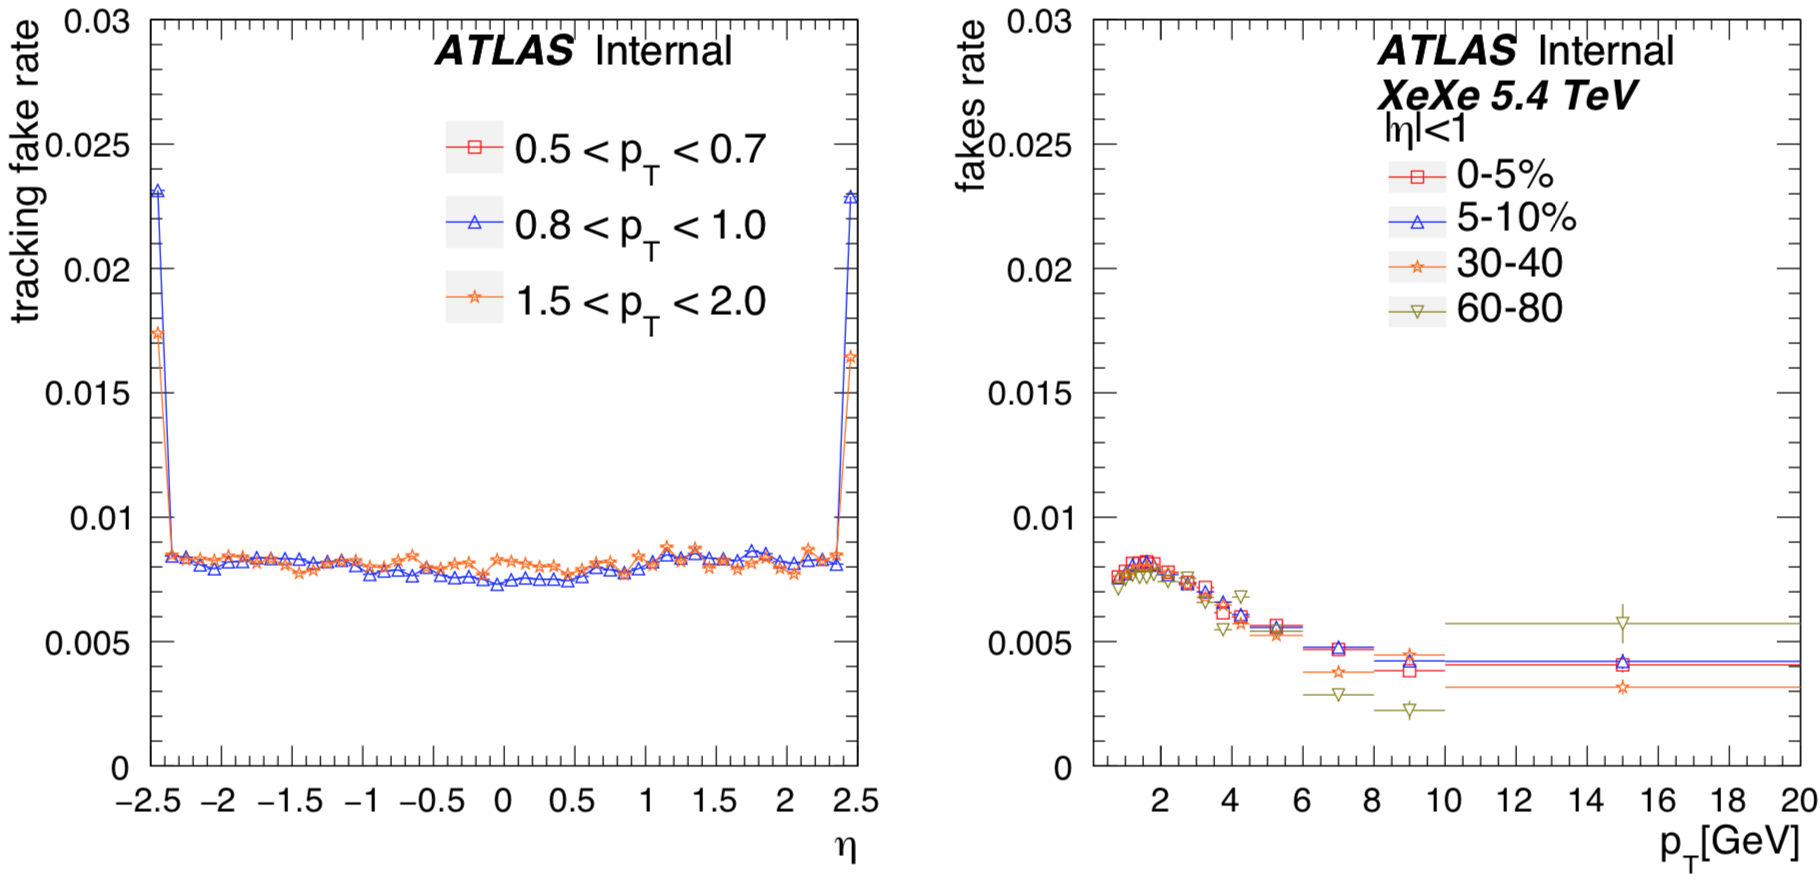
\includegraphics[width=.95\linewidth]{figs/chapter_detector/ATLAS_track_fake_XeXe544.png}
\caption{Fake rates as a function of $\eta$ (left) and $\pT$ (right) for selected centrality and $\pT$ ranges. The $\eta$ dependence is shown for $10\%$ most central events, where fake rate is highest.}
\label{fig:detector_ATLAS_track_fake_XeXe544}
\end{figure}



\subsubsection{$p$+Pb at $\sqrt{s}=5.02$ TeV}

$p$+Pb data at $\sqrt{s}=5.02$ TeV data have been collected in 2013 (Run 1) and 2016 (Run 2). Since the event and tracking selections are quite different between Run 1 and Run 2, they will be discussed separately in the following sections.



\paragraph{Trigger}

The triggers applied in 5.02 TeV $p$+Pb have two parts: MinBias and High Multiplicity Track (HMT). A list of all the major MinBias and HMT triggers used in 2013 is summarized as follows:
\begin{itemize}
\item \verb|EF_mbMbts_1_1_counter|
\item \verb|EF_hip_trkX_TEY_counter|
\end{itemize}
where two new algorithms are used:
\begin{itemize}
\item \verb|mbMbts_1_1|: HLT trigger requires at least 1 hit on both sides of MBTS;
\item \verb|trkX|: HLT trigger requires at least X online reconstructed tracks;
\end{itemize}
The threshold combinations $(X, Y)$ for number of tracks (\verb|trk|) and total energy (\verb|TE|) are (100, 10), (130, 10), (150, 50), (185, 50), (200, 65) and (225, 65).

A summary of statistics with all the major triggers used in this thesis are shown in Figure~\ref{fig:detector_ATLAS_trigger_pPb2013}.
\begin{figure}[H]
\centering
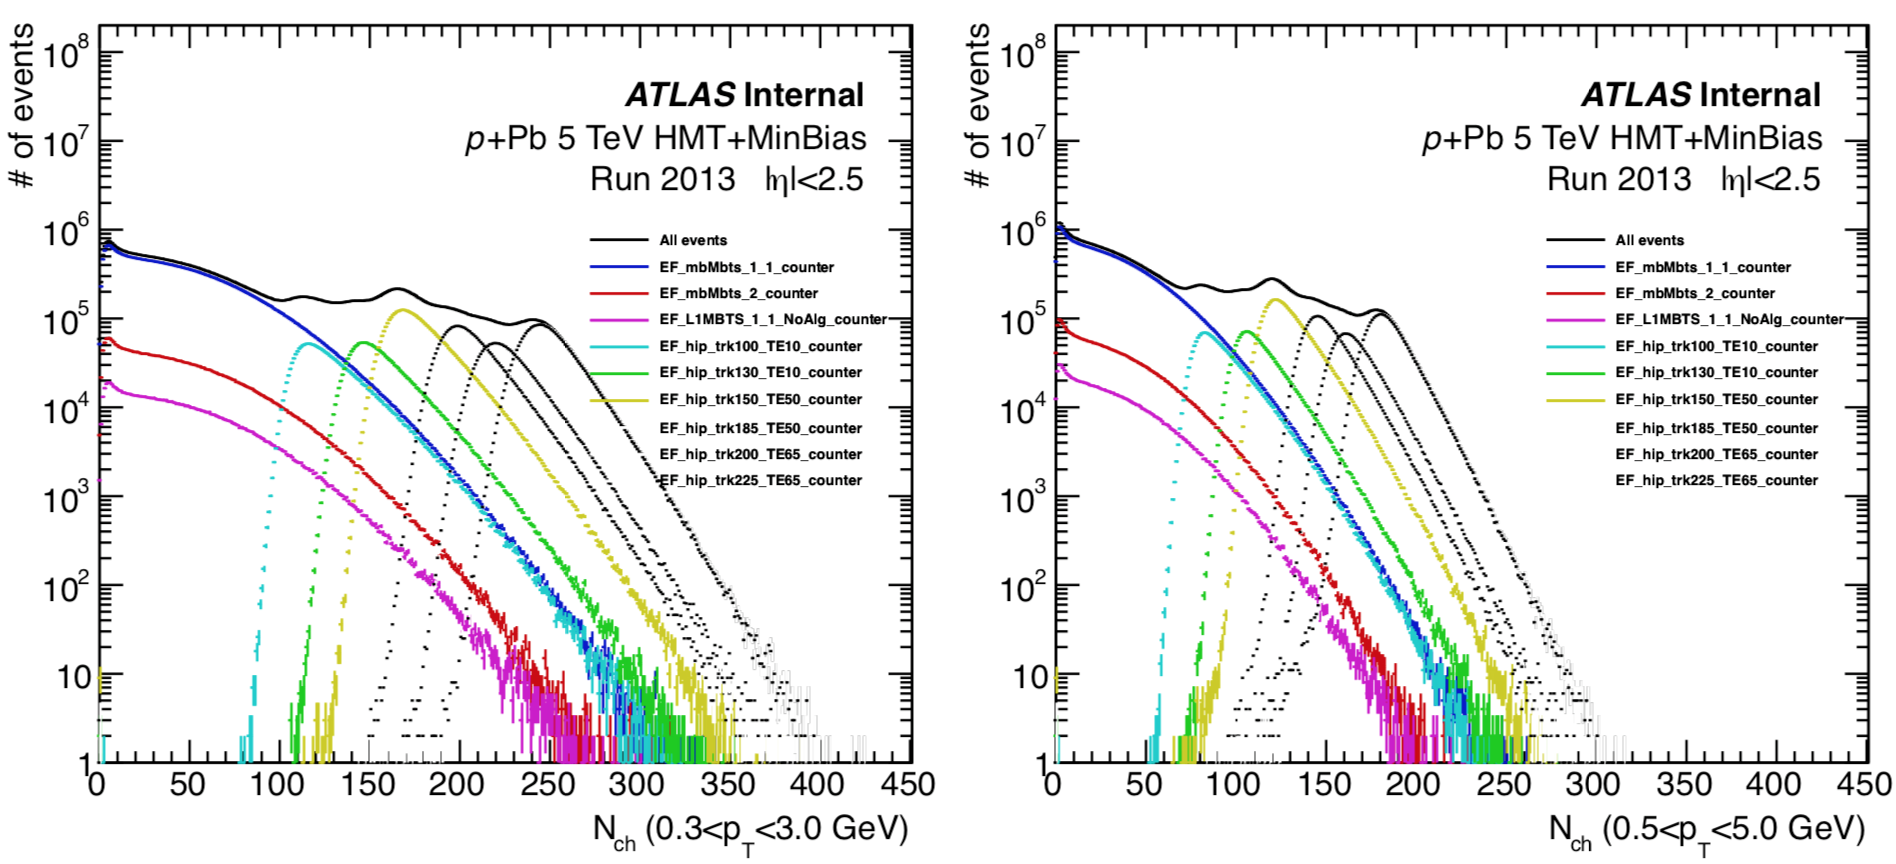
\includegraphics[width=.95\linewidth]{figs/chapter_detector/ATLAS_trigger_pPb2013.png}
\caption{Distributions of number of tracks with two $\pT$ thresholds, for 5.02 TeV $p$+Pb run in 2013. The major MinBias and HMT triggers are plotted separately.}
\label{fig:detector_ATLAS_trigger_pPb2013}
\end{figure}

Due to the reason that the intermediate $\Nchrec$ region is not covered by the 2013 HMT triggers, several new HMT triggers with intermediate $\Nchrec$ thresholds are specially designed for the 2016 data taking. Together with MinBias triggers, all the major triggers used in this thesis are summarized as follows:
\begin{itemize}
\item \verb|HLT_noalg_mb_L1MBST_1|
\item \verb|HLT_noalg_mb_L1MBST_1_1|
\item \verb|HLT_mb_sp100_trkX_hmt_L1MBST_1_1|
\end{itemize}
where all the HMT triggers are seeded on \verb|L1MBTS_1_1|, which is different from 2013 since the luminosity is much lower. The new algorithms are:
\begin{itemize}
\item \verb|L1MBST_1| requires at least one hit in one of the MBST detectors;
\item \verb|L1MBST_1_1| requires at least one hit in both of the MBST detectors;
\item \verb|sp100| requires at least 100 space points in for the HLT track reconstruction.
\end{itemize}
The thresholds $X$ for number of tracks (\verb|trk|) are 10, 20, 30, 60, 80, 100 and 110.

The summary of statistics with all the major triggers used in this thesis are shown in Figure~\ref{fig:detector_ATLAS_trigger_pPb2016}.
\begin{figure}[H]
\centering
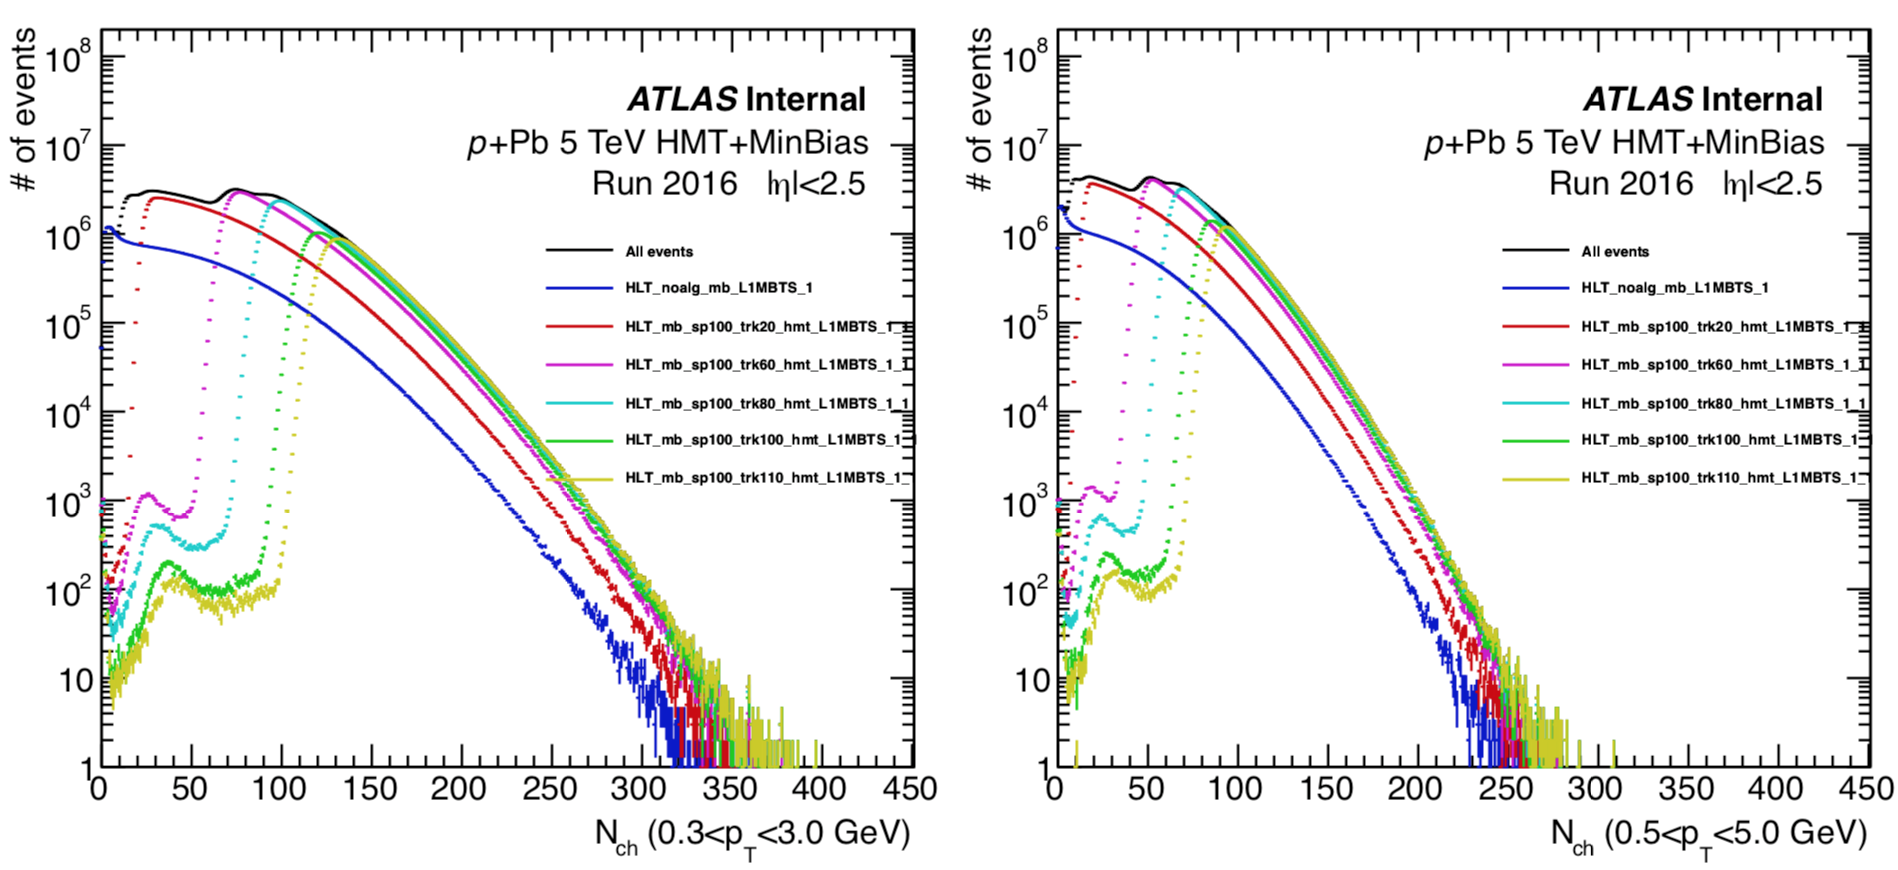
\includegraphics[width=.95\linewidth]{figs/chapter_detector/ATLAS_trigger_pPb2016.png}
\caption{Distributions of number of tracks with two $\pT$ thresholds, for 5.02 TeV $p$+Pb run in 2016. The major MinBias and HMT triggers are plotted separately.}
\label{fig:detector_ATLAS_trigger_pPb2016}
\end{figure}



\paragraph{Event selection}

In 2013, low-$\mu$ 5.02 TeV $p$+Pb data were collected with the ATLAS detectors. Each event is required to pass the following cuts:
\begin{itemize}
\item Good run list;
\item A primary reconstructed vertex with $z_\text{vtx}<100$ mm;
\item MBTS timing cuts
\begin{itemize}
\item $|\text{time}_\text{A}|$ or $|\text{time}_\text{C}|$ must not be equal to 75 or 0 ns;
\item $|\text{time}_\text{A} - \text{time}_\text{C}|<10$ ns;
\end{itemize}
\end{itemize}
and the pileup events are suppressed by rejecting events containing more than one good reconstructed vertex. The remaining pileup events are further suppressed based on the signal in the ZDC on the Pb-fragmentation side. This signal is calibrated to the number of detected neutrons $N_\text{n}$ based on the location of the peak corresponding to a single neutron. The distribution of $N_\text{n}$ in events with pileup is broader than that for events without pileup. Hence, a simple cut on the high tail end of the ZDC signal distribution further suppresses the pileup, which retaining more than $98\%$ of the events without pileup. After this pileup rejection procedure, the residual fraction is estimated to be $1\%$ in the event class with the highest track multiplicity studied in this analysis.

In 2016, 5.02 TeV $p$+Pb data was collected with lower $\mu$ value than 2013. In addition to the event selections in 2013 (without MBTS timing cuts), events with problematic detectors are also removed. Since $\mu$ value of 2016's run is much lower than 2013's, cleaning pileup events is not crucial.



\paragraph{Track selection, efficiency and fake rate}

The track selection criteria for 2016 $p$+Pb is quite different from Pb+Pb. The analysis uses the $p$+Pb data reprocessed with the tracking extended down to 0.1 GeV:
\begin{itemize}
\item Present hit in B-Layer if expected
\item Number of Pixel hits $\geq 1$
\item SCT hits:
\begin{itemize}
\item SCT hits $\geq$ 2 for $0.1 < \pT < 0.2$ GeV
\item SCT hits $\geq$ 4 for $0.2 < \pT < 0.3$ GeV
\item SCT hits $\geq$ 6 for $\pT > 0.3$ GeV
\end{itemize}
\item significance cuts:
\begin{itemize}
\item $|\frac{d_0}{err_{d_0}}|<3$
\item $|\frac{z_0\sin\theta}{err_{z_0\sin\theta}}|<3$
\end{itemize}
\end{itemize}

Tracking efficiency is estimated in a similar way as Pb+Pb. The tracking efficiency evaluated as a function of $\eta$ for different $\pT$ ranges compared between different multiplicity ranges are shown in Figure~\ref{fig:detector_ATLAS_track_eff_pPb}. The efficiency is lower in the lowest $\pT$ range ($0.1<\pT<0.2$ GeV), but changes weakly with increase in the $\pT$ above that. The $\eta$ dependence of the efficiency is also different the lowest $\pT$ range, but remains nearly consistent in the highest $\pT$ ranges. The $\eta$ dependence of the efficiency is also much weaker than that seen in central Pb+Pb collisions. Efficiency shows very weak dependence with multiplicity although the lowest multiplicity ranges shows a lightly lower efficiency than the rest of the multiplicity ranges.

\begin{figure}[H]
\centering
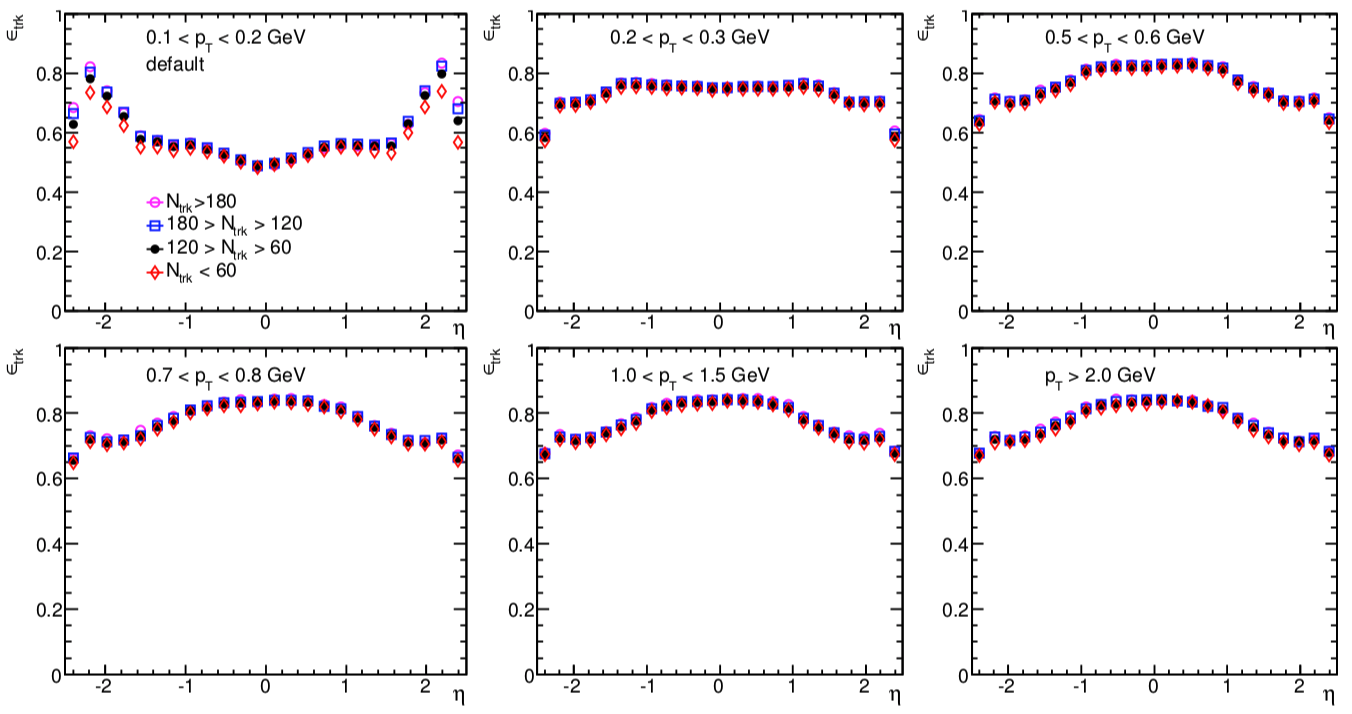
\includegraphics[width=.95\linewidth]{figs/chapter_detector/ATLAS_track_eff_pPb.png}
\caption{Tracking efficiency $\epsilon$ as a function of $\eta$ for default selection requirements for different transverse momentum $\pT$ ranges compared between different multiplicity bins, for $p$+Pb.}
\label{fig:detector_ATLAS_track_eff_pPb}
\end{figure}



\subsubsection{$pp$ at $\sqrt{s}=13$ TeV}

In 2015 and 2016, low-$\mu$ and intermediate-$\mu$ $pp$ data was collected by ATLAS detectors. An additional pixel layer, the ``Insertable B Layer'' (IBL) installed between Run 1 and Run 2, is used in the $pp$ measurement. There are four run periods depending on the triggers and will be discussed below.



\paragraph{Trigger}

The triggers that have been used in this analysis have both MinBias and HMT triggers. The HMT triggers are developed to enhance event statistics in high multiplicity region. Since the main uncertainty in many measurements, like cumulants, are from statistical errors, HMT triggers are crucial in order to extend the measurement to higher multiplicity region. The list of all major triggers used are listed as follows:
\begin{itemize}
\item \verb|HLT_mb_sptrk|
\item \verb|HLT_noalg_mb_MBTS_1|
\item \verb|HLT_noalg_mb_MBTS_1_1|
\item \verb|HLT_mb_mbts_L1MBTS_1_1|
\item \verb|HLT_mb_sp400_trk40_hmt_L1MBTS_1_1|
\item \verb|HLT_mb_sp900_trk50_hmt_L1TE5|
\item \verb|HLT_mb_sp900_trk60_hmt_L1MBTS_1_1|
\item \verb|HLT_mb_sp1000_trk70_hmt_L1TE5|
\item \verb|HLT_mb_sp1400_trk90_hmt_L1TE10|
\end{itemize}

Figure~\ref{fig:detector_ATLAS_trigger_pp13} shows the distributions of number of tracks from two $\pT$ thresholds: $0.3<\pT<3.0$ GeV (left panel) and $0.5<\pT<5.0$ GeV (right panel). Due to a large number of HMT triggers, only selected triggers are shown.

\begin{figure}[H]
\centering
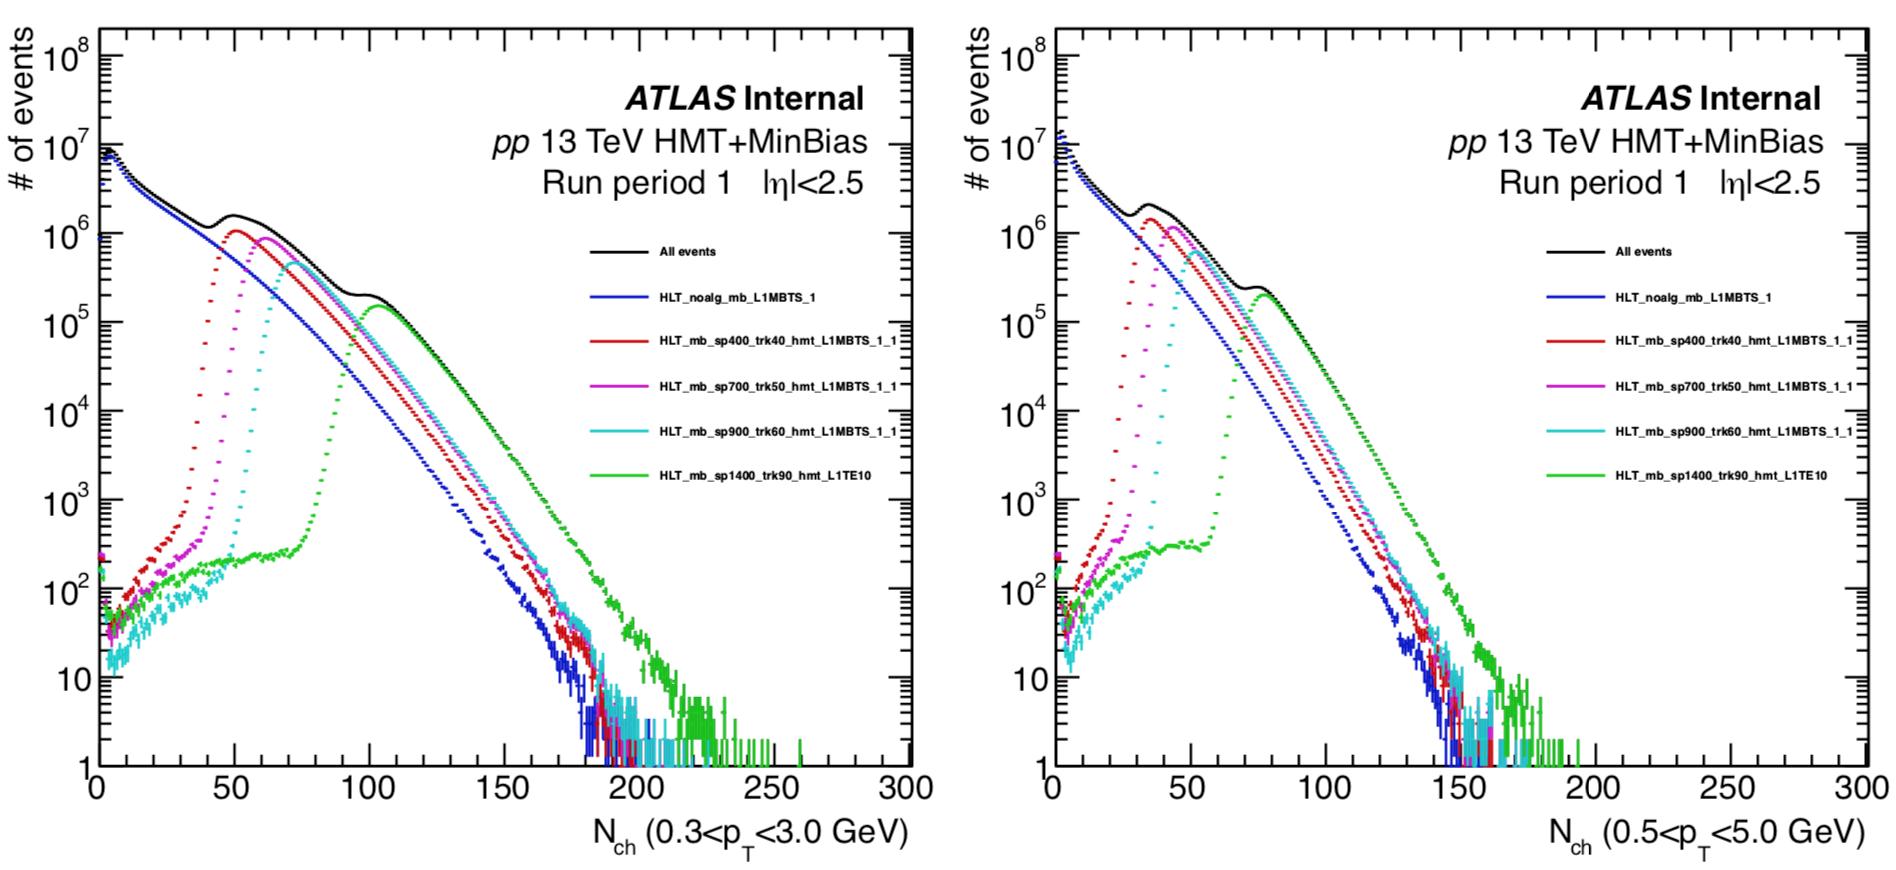
\includegraphics[width=.95\linewidth]{figs/chapter_detector/ATLAS_trigger_pp13.png}
\caption{Distributions of number of tracks with two $\pT$ thresholds, in 13 TeV $pp$, with selected MinBias and HMT triggers. "All events" means all the MinBias and HMT triggers combined.}
\label{fig:detector_ATLAS_trigger_pp13}
\end{figure}



\paragraph{Event selection}

The event selection criteria for $pp$ are exactly the same as Pb+Pb at $\sqrt{s_\text{NN}}=5.02$ TeV, see Section~\ref{sec:event_selection} for details.



\paragraph{Track selection, efficiency and fake rate}

The track selection for $pp$ is slightly different from $p$+Pb:
\begin{itemize}
\item If IBL hit is expected: at least 1 IBL hit;
\item If no IBL hit is expected: a Layer-0 hit if expected;
\item At least 1 pixel hit + dead sensors;
\item SCT hits:
\begin{itemize}
\item $\pT<0.3$ GeV: at least 2 SCT hits + dead sensors;
\item $\pT<0.4$ GeV: at least 4 SCT hits + dead sensors;
\item $\pT>0.4$ GeV: at least 6 SCT hits + dead sensors;
\end{itemize}
\item If $\pT>10$ GeV: $\chi^2$ probability < 0.01;
\item $|d_0|<1.5$;
\item $|z_0-z_\text{vtx}|\sin\theta<1.5$;
\end{itemize}

The PYTHIA A2 tune was used to produce $pp$ collisions with the same energy as in the data. The detector response is simulated with GEANT 4 with conditions matching those present during the data-taking. The simulated events are reconstructed with the same algorithms as data, in particular using the same track reconstruction as for the data.

The definitions of tracking efficiency and fake rates are identical to the Pb+Pb collision system (Section~\ref{sec:track_selection_efficiency_and_fake_rate}). The tracking efficiency is shown in Figure~\ref{fig:detector_ATLAS_track_eff_pp13}. The boundaries of $\Nchrec$ are chosen to make each $\Nchrec$ range contain enough statistics for the efficiency measurement. The efficiency is higher in high multiplicity. Linear interpolation is applied in data analysis to obtain more precise efficiency in cases when $\pT$ or $\eta$ are not in the bin center.
\begin{figure}[H]
\centering
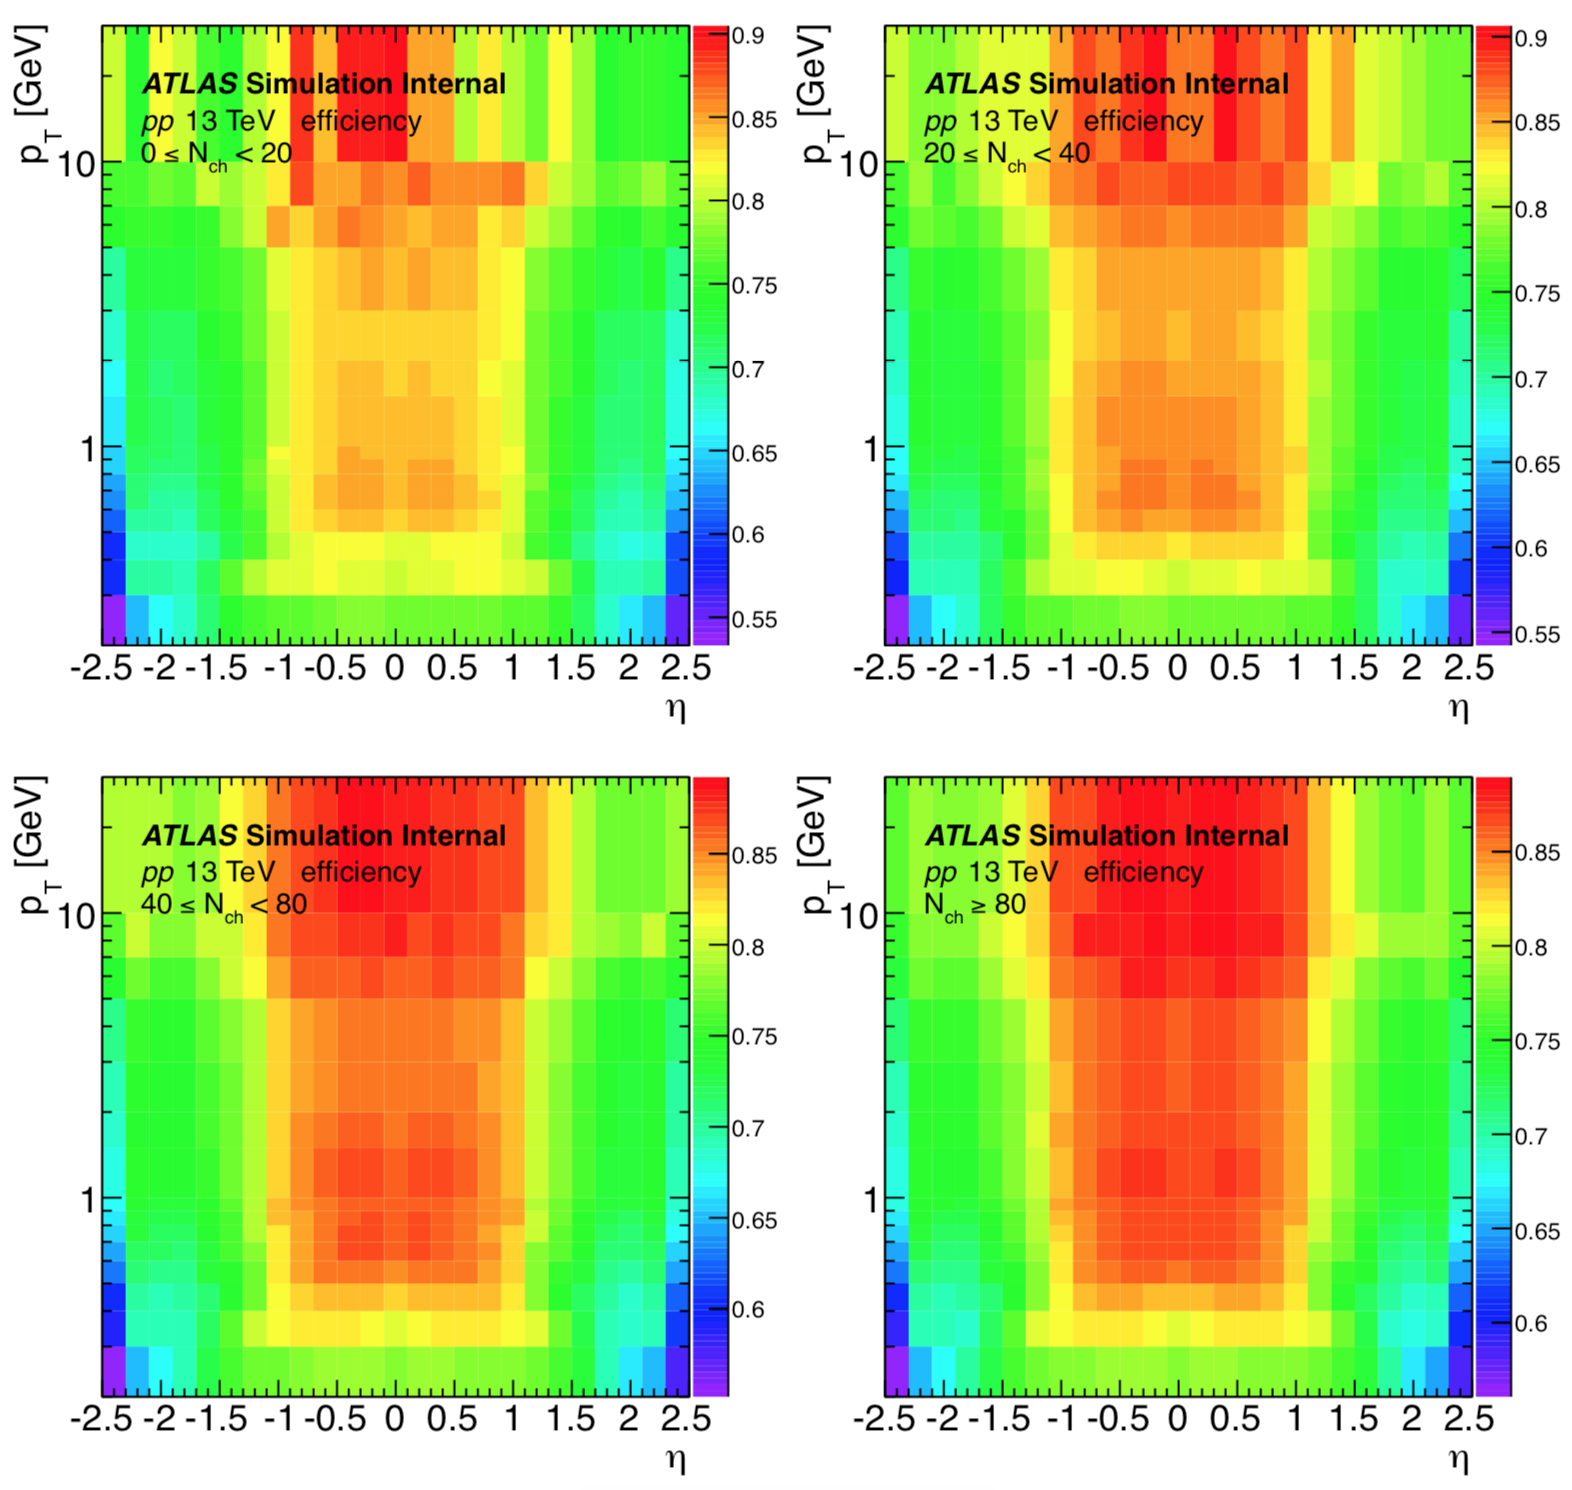
\includegraphics[width=.95\linewidth]{figs/chapter_detector/ATLAS_track_eff_pp13.png}
\caption{Tracking efficiency $\epsilon(\eta, \pT)$. Different panels are for different $\Nchrec$ ranges.}
\label{fig:detector_ATLAS_track_eff_pp13}
\end{figure}

The fake rates are shown in Figure~\ref{fig:detector_ATLAS_track_fake_pp13}, where four panels are for four different $\Nchrec$ ranges, respectively. Since the maximum fake rate is smaller than the level of $0.1\%$, even for the lowest $\pT$, unlike central Pb+Pb, fake rates have no impact on the $pp$ data analysis.
\begin{figure}[H]
\centering
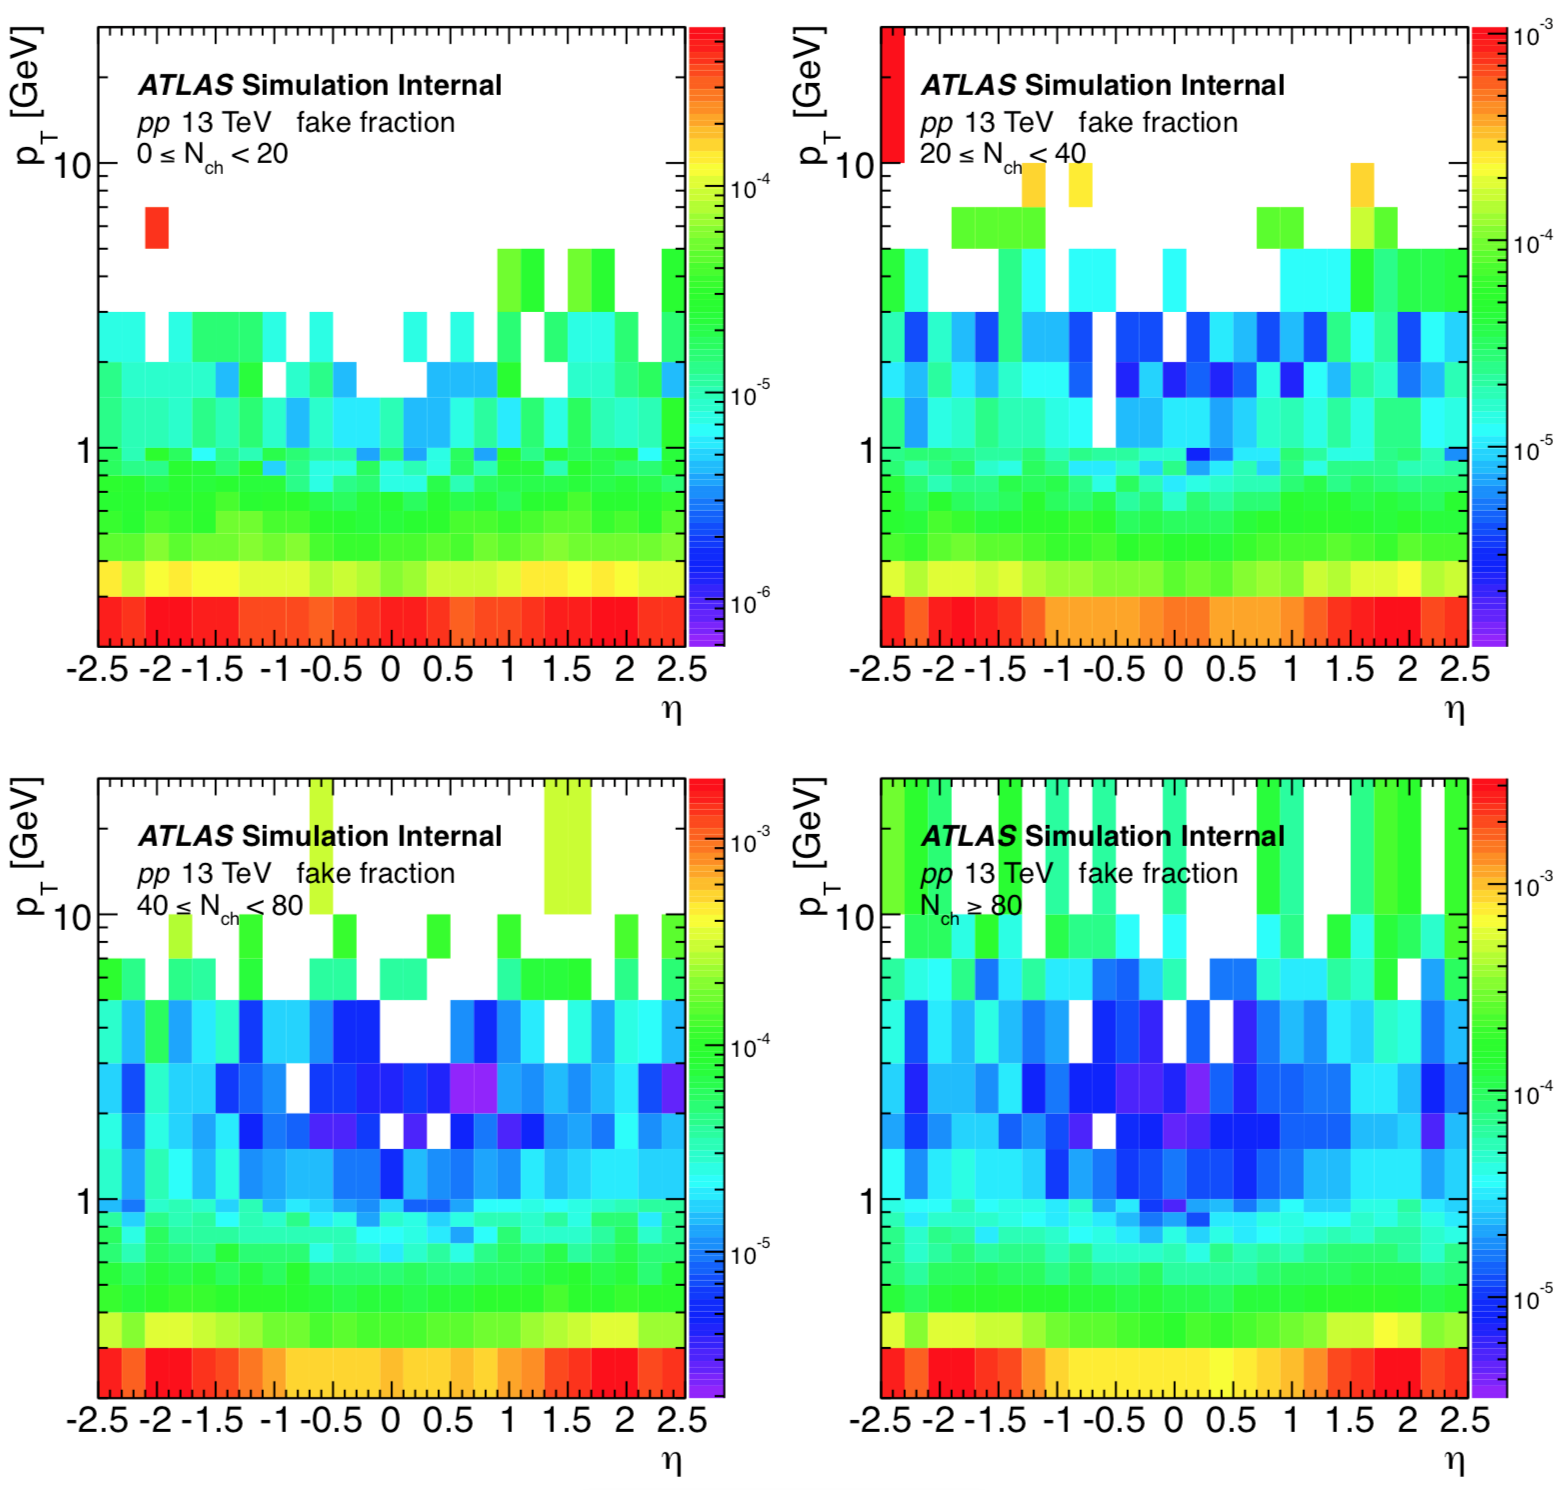
\includegraphics[width=.95\linewidth]{figs/chapter_detector/ATLAS_track_fake_pp13.png}
\caption{Fake rates $f(\eta, \pT)$. Different panels are for different $\Nchrec$ ranges.}
\label{fig:detector_ATLAS_track_fake_pp13}
\end{figure}



